% !TeX document-id = {71c6af50-c6d7-4a14-89e8-2089cc2c8bd7}
% % Konfiguration für Texstudio (Version > 2.9)
% !TeX program = xelatex
% !TeX TXS-program:compile = txs:///xelatex/[-8bit]
% !BIB program = biber
% !TeX spellcheck = en_US
% !TeX encoding = utf8

\documentclass[a4paper, titlepage]{article}
\usepackage{a4wide}	% smaller borders
\usepackage{titling}

\def\modern{
	\usepackage{fontspec}
	\defaultfontfeatures{
      Ligatures=TeX,
      Numbers=OldStyle,
      Mapping=tex-text,
      SmallCapsFeatures={LetterSpace=8, Numbers=OldStyle}
	}
	% \setmainfont{Gentium Book Basic}
}

% do not split this line in more lines, otherwise "make git-manual" will show the wrong version
\usepackage[siunitx, RPvoltages]{circuitikz}
% Let this be the same as the chosen voltage direction for coherence
\def\chosenvoltoption{RPvoltages}

\usepackage{ifxetex,ifluatex}
\ifxetex
	\modern
\else
	\ifluatex
		\modern
	\else
	% pdflatex
		\usepackage[T1]{fontenc}
		\usepackage[utf8]{inputenc}
		% \usepackage{babel}
	\fi
\fi
\def\tightlist{} % needed for latest pandoc-versions(pandoc used for including changelog)
\usepackage{microtype}

\sisetup{load=derived} % loading \siemens
\usepackage{showexpl}
%
% The following trick is used to silence showexpl a bit, so that the
% logs are readable...
%
\makeatletter
\let\SX@Info=\relax % silence showexpl a bit...
\makeatother
%
\lstset{
    pos=l,
    width=-99pt,
    overhang=0pt,
    hsep=\columnsep,
    vsep=\bigskipamount,
    rframe=single,
    numbers=left,
    numberstyle=\tiny,
    numbersep=.3em,
    xleftmargin=1em,
    columns=flexible,
    language=[LaTeX]TEX,breaklines=true,
    basicstyle=\normalsize\ttfamily,tabsize=3
}

\usepackage{booktabs}
\renewcommand{\arraystretch}{1.2}

\usepackage{framed, xtab}
\usepackage{hyperref}
\hypersetup{
    bookmarks=false,         % show bookmarks bar?
    pdftitle={CircuiTikZ \pgfcircversion\ - manual}, % title
    pdfauthor={Massimo Redaelli, Stefan Lindner, Stefan Erhardt, Romano Giannetti}, % authors
    pdfsubject={CircuiTikZ manual},   % subject of the document
    pdfkeywords={},   % list of keywords
    colorlinks=true,  % false: boxed links; true: colored links
    linkcolor=blue,   % color of internal links
    citecolor=blue,   % color of links to bibliography
    filecolor=blue,   % color of file links
    urlcolor=blue     % color of external links
}
\usepackage{imakeidx}
\usepackage{textcomp}
\makeindex[title=Index of the components, intoc=true]

% Local utilities packages
\usepackage{ctikzmanutils}

\newcommand{\email}[1]{\href{mailto:#1}{#1}}
\long\def\comment#1{}

% There are a lot of boxes in the document; let's try to give TeX
% a bit of leverage... do not use parindent (which looks strange between examples)
% and add stretch between paragraph, to avoid a lot of sections and subsections
% starting at the end of the page.
\parindent=0pt
\parskip=4pt plus 6pt minus 2pt

\begin{document}
\setcounter{secnumdepth}{4}
\setcounter{tocdepth}{4}

\def\TikZ{Ti\emph{k}Z}
\def\Circuitikz{Circui\TikZ}
\def\ConTeXt{Con\TeX t}
\lstset{frameround=fttt}
\lstloadlanguages{TeX}

\title{\Circuitikz \\{\large version \pgfcircversion{} (\pgfcircversiondate)}}
\author{Massimo A. Redaelli (\email{m.redaelli@gmail.com})\\
    Stefan Lindner (\email{stefan.lindner@fau.de})\\
    Stefan Erhardt (\email{stefan.erhardt@fau.de})\\
    Romano Giannetti (\email{romano.giannetti@gmail.com})}
\date{\today}

\pretitle{\begin{center}%
    \begin{circuitikz}
        \draw (0,0) node[dipchip, rotate=90, num pins=40, fill=cyan!20!white](C){%
            \rotatebox{-90}{\LARGE\Circuitikz}%
        };
        \draw (C.pin 20) -- ++(0,-8) node[ground](GND){};
        \draw (C.pin 7) to[D, fill=blue] ++(0,-1) -- ++(0.5,0) to[R] ++(2,0)
            coordinate(a1) to[short, -*]
            node[above left, blue]{Massimo A. Redaelli}
            node[below left,]{\email{m.redaelli@gmail.com}}
            (a1-|GND);
            \draw (C.pin 5) to[D, fill=red] ++(0,-3)-- ++(0.5,0) to[R] ++(2,0)
            coordinate(a2) to[short, -*]
            node[above left, blue]{Stefan Lindner}
            node[below left,]{\email{stefan.lindner@fau.de}}
            (a2-|GND);
            \draw (C.pin 3) to[D, fill=green] ++(0,-5)-- ++(0.5,0) to[R] ++(2,0)
            coordinate(a3) to[short, -*]
            node[above left, blue]{Stefan Erhart}
            node[below left,]{\email{stefan.erhardt@fau.de}}
            (a3-|GND);
            \draw (C.pin 1) to[D, fill=yellow] ++(0,-7)-- ++(0.5,0) to[R] ++(2,0)
            coordinate(a4) to[short, -*]
            node[above left, blue]{Romano Giannetti}
            node[below left,]{\email{romano.giannetti@gmail.com}}
            (a4-|GND);
    \end{circuitikz}
    \par\bigskip\vfill}
\posttitle{\end{center}}

\maketitle

\tableofcontents
\cleardoublepage
\section{Introduction}
\subsection{About}
\Circuitikz\ was initiated by Massimo Redaelli in 2007, who was working as a research assistant at the Polytechnic University of Milan, Italy, and needed a tool for creating exercises and exams.
After he left University in 2010 the development of \Circuitikz\ slowed down, since \LaTeX\ is mainly established in the academic world. In 2015 Stefan Lindner and Stefan Erhardt, both working as research assistants at the University of Erlangen-Nürnberg, Germany, joined the team and now maintain the project together with the initial author. In 2018 Romano Giannetti, full professor of Electronics at Comillas Pontifical University of Madrid, joined the team.

The use of \Circuitikz\ is, of course, not limited to academic teaching. The package gets widely used by engineers for typesetting electronic circuits for articles and publications all over the world.

\subsection{License}
Copyright \copyright\ 2007--2019 Massimo Redaelli. This package is author-maintained. Permission is granted to copy, distribute and/or modify this software under the terms of the \LaTeX\ Project Public License, version 1.3.1, or the GNU Public License. This software is provided ‘as is’, without warranty of any kind, either expressed or implied, including, but not limited to, the implied warranties of merchantability and fitness for a particular purpose.
\subsection{Loading the package}

\begin{table}[h]
\centering
\begin{tabular}{ll}\toprule
	\LaTeX       	& \ConTeXt\footnotemark \\ \midrule
	\verb!\usepackage{circuitikz}!	& \verb!\usemodule[circuitikz]!\\
	\bottomrule
\end{tabular}
\end{table}
\footnotetext{\ConTeXt\ support was added mostly thanks to Mojca Miklavec and Aditya Mahajan.}

\noindent \TikZ\ will be automatically loaded.

\noindent Circui\TikZ\ commands are just \TikZ\ commands, so a minimum usage example would be:

\begin{LTXexample}[varwidth=true]
\tikz \draw (0,0) to[R=$R_1$] (2,0);
\end{LTXexample}

\subsection{Installing a new version of the package.}

The stable version of the package should come with your \LaTeX\ distribution. Downloading the files from CTAN and installing them locally is, unfortunately, a distribution-dependent task and sometime not so trivial. If you search for \texttt{local texmf tree} and the name of your distribution on \url{https://tex.stackexchange.com/} you will find a lot of hints.

Anyway, the easiest way of using whichever version of \Circuitikz\ is to point to the github page \url{https://circuitikz.github.io/circuitikz/} of the project, and download the version you want. You will download a simple (biggish) file, called \texttt{circuitikz.sty}.

Now you can just put this file in your local \texttt{texmf} tree, if you have one, or simply adding it into the same directory where your main file resides, and then use

\begin{verbatim}
    \usepackage[...options...]{circuitikzgit}
\end{verbatim}

instead of \texttt{circuitikz}. This is also advantageous for ``future resilience''; the authors try hard not to break backward compatibility with new versions, but sometime things happen.

\subsection{Requirements}
\begin{itemize}
    \item \texttt{tikz}, version $\ge 3$;
    \item \texttt{xstring}, not older than 2009/03/13;
    \item \texttt{siunitx}, if using \texttt{siunitx} option.
\end{itemize}

\subsection{Incompatible packages}
\TikZ's own \texttt{circuit} library, which is based on \Circuitikz, (re?)defines several styles used by this library. In order to have them work together you can use the \texttt{compatibility} package option, which basically prefixes the names of all \Circuitikz\ \texttt{to[]} styles with an asterisk.

So, if loaded with said option, one must write \verb!(0,0) to[*R] (2,0)! and, for transistors on a path, \verb!(0,0) to[*Tnmos] (2,0)!, and so on (but \verb!(0,0) node[nmos] {}!). See example at page~\pageref{ex:compatibility}.

\subsection{Known bugs and limitation}\label{sec:bugs}

\Circuitikz{} will \textbf{not work} correctly with global (in the main \texttt{circuitikz} environment, or in \texttt{scope} environments) \emph{negative} scale parameters (\texttt{scale}, \texttt{xscale} or \texttt{yscale}), unless \texttt{transform shape} is also used, and even in this cases the behavior is not guaranteed.
Neither it will work with angle-changing scaling (when \texttt{xscale} is different form \texttt{yscale}) and with the global \texttt{rotate} parameter.

Correcting this will need a big rewrite of the path routines, and although the authors are thinking about solving it, don't hold your breath; it will need changing a lot of interwoven code (labels, voltages, currents and so on). Contributions and help would be highly appreciated.

This same issue create a lot of problem of compatibility between \Circuitikz{} and the new \texttt{pic} Ti\emph{k}Z feature, so basically don't put components into \texttt{pic}s.


\subsection{Incompabilities between version}
Here, we will provide a list of incompabilitys between different version of circuitikz. We will try to hold this list short, but sometimes it is easier to break with old syntax than including a lot of switches and compatibility layers.
You can check the used version at your local installation using the macro \verb!\pgfcircversion{}!.
\begin{itemize}
    \item After v0.9.0: the parameters \texttt{tripoles/american or port/aaa}, \texttt{...bbb}, \texttt{...ccc} and \texttt{...ddd} are no longer used and are silently ignored; the same stands for \texttt{nor}, \texttt{xor}, and \texttt{xnor} ports.
    \item After v0.9.0: voltage and current directions/sign (plus and minus signs in case of \texttt{american voltages} and arrows in case of \texttt{european voltages} have been rationalized with a couple of new options (see details in section~\ref{curr-and-volt}. The default case is still the same as v0.8.3.
    \item Since v0.8.2: voltage and current label directions(v<= / i<=) do NOT change the orientation of the drawn source shape anymore. Use the "invert" option to rotate the shape of the source. Furthermore, from this version on, the current label(i=) at current sources can be used independent of the regular label(l=).
    \item Since v0.7?: The label behaviour at mirrored bipoles has changes, this fixes the voltage drawing, but perhaps you have to adjust your label positions.
    \item Since v0.5.1: The parts pfet, pigfete, pigfetebulk and pigfetd are now mirrored by default. Please adjust your yscale-option to correct this.
    \item Since v0.5: New voltage counting direction, here exists an option to use the old behaviour
\end{itemize}

If you have older projects that show compatibility problems, you have two options:
\begin{itemize}
    \item you can use an older version locally using the git-version and picking the correct commit from the repository (branch gh-pages) or the main GitHub site directly;
    \item if you are using \LaTeX, the distribution has embedded several important old versions: \texttt{0.4}, \texttt{0.6}, \texttt{0.7} and \texttt{0.8.3}. To switch to use them, you simply change your \verb|\usepackage| invocation like
        \begin{lstlisting}
            \usepackage[]{circuitik-0.8.3} % or circuitikz-0.4, 0.6...
        \end{lstlisting}
    You have to take care of the options that may have changed between versions;
    \item   if you are using  \ConTeXt, only version \texttt{0.8.3} is packaged for now; if can use it with
        \begin{lstlisting}
            \usemodule[circuitik-0.8.3]
        \end{lstlisting}
\end{itemize}


\subsection{Feedback}
The easiest way to contact the authors is via the official Github repository: \url{https://github.com/circuitikz/circuitikz/issues}

\subsection{Package options}
\label{sec:package-options}

\noindent Circuit people are very opinionated about their symbols. In order to meet the individual gusto you can set a bunch of package options. The standard options are what the authors like, for example you get this:
\begin{LTXexample}[varwidth=true]
    \begin{circuitikz}
        \draw (0,0) to[R=2<\ohm>, i=?, v=84<\volt>] (2,0) --
        (2,2) to[V<=84<\volt>] (0,2)
        -- (0,0);
    \end{circuitikz}
\end{LTXexample}

Feel free to load the package with your own cultural options:

\begin{center}
    \begin{tabular}{ll}\toprule
        \LaTeX                & \ConTeXt \\ \midrule
        \verb!\usepackage[american]{circuitikz}! & \verb!\usemodule[circuitikz][american]!\\
        \bottomrule
    \end{tabular}
\end{center}

\begin{LTXexample}[varwidth=true,linerange={1-1,3-6}]
    \begin{circuitikz}
        [circuitikz/voltage=american, circuitikz/resistor=american] % line not printed
        \draw (0,0) to[R=2<\ohm>, i=?, v=84<\volt>] (2,0) --
        (2,2) to[V<=84<\volt>] (0,2)
        -- (0,0);
    \end{circuitikz}
\end{LTXexample}

\medskip{}

\noindent Here is the list of all the options:
{\sloppy % for the big lists of \texttt here
    \begin{itemize}
        \item \texttt{europeanvoltages}: uses arrows to define voltages, and uses european-style voltage sources;
        \item \texttt{straightvoltages}: uses arrows to define voltages, and and uses straight voltage arrows;
        \item \texttt{americanvoltages}: uses $-$ and $+$ to define voltages, and uses american-style voltage sources;
        \item \texttt{europeancurrents}: uses european-style current sources;
        \item \texttt{americancurrents}: uses american-style current sources;
        \item \texttt{europeanresistors}: uses rectangular empty shape for resistors, as per european standards;
        \item \texttt{americanresistors}: uses zig-zag shape for resistors, as per american standards;
        \item \texttt{europeaninductors}: uses rectangular filled shape for inductors, as per european standards;
        \item \texttt{americaninductors}: uses "4-bumps" shape for inductors, as per american standards;
        \item \texttt{cuteinductors}: uses my personal favorite, "pig-tailed" shape for inductors;
        \item \texttt{americanports}: uses triangular logic ports, as per american standards;
        \item \texttt{europeanports}: uses rectangular logic ports, as per european standards;
        \item \texttt{americangfsurgearrester}: uses round gas filled surge arresters, as per american standards;
        \item \texttt{europeangfsurgearrester}: uses rectangular gas filled surge arresters, as per european standards;
        \item \texttt{european}: equivalent to \texttt{europeancurrents}, \texttt{europeanvoltages}, \texttt{europeanresistors}, \texttt{europeaninductors}, \texttt{europeanports}, \texttt{europeangfsurgearrester};
        \item \texttt{american}: equivalent to \texttt{americancurrents}, \texttt{americanvoltages}, \texttt{americanresistors}, \texttt{americaninductors}, \texttt{americanports}, \texttt{americangfsurgearrester};
        \item \texttt{siunitx}: integrates with \texttt{SIunitx} package. If labels, currents or voltages are of the form \verb!#1<#2>! then what is shown is actually \verb!\SI{#1}{#2}!;
        \item \texttt{nosiunitx}: labels are not interpreted as above;
        \item \texttt{fulldiode}: the various diodes are drawn \emph{and} filled by default, i.e. when using styles such as \texttt{diode}, \texttt{D}, \texttt{sD}, \ldots Other diode styles can always be forced with e.g. \texttt{Do}, \texttt{D-},  \ldots
        \item \texttt{strokediode}: the various diodes are drawn \emph{and} stroke by default, i.e. when using styles such as \texttt{diode}, \texttt{D}, \texttt{sD}, \ldots Other diode styles can always be forced with e.g. \texttt{Do}, \texttt{D*},  \ldots
        \item \texttt{emptydiode}: the various diodes are drawn \emph{but not} filled by default, i.e. when using styles such as \texttt{D}, \texttt{sD}, \ldots Other diode styles can always be forced with e.g. \texttt{Do}, \texttt{D-},  \ldots
        \item \texttt{arrowmos}: pmos and nmos have arrows analogous to those of pnp and npn transistors;
        \item \texttt{noarrowmos}: pmos and nmos do not have arrows analogous to those of pnp and npn transistors;
        \item \texttt{fetbodydiode}: draw the body diode of a FET;
        \item \texttt{nofetbodydiode}: do not draw the body diode of a FET;
        \item \texttt{fetsolderdot}: draw solderdot at bulk-source junction of some transistors;
        \item \texttt{nofetsolderdot}: do not draw solderdot at bulk-source junction of some transistors;
        \item \texttt{emptypmoscircle}: the circle at the gate of a pmos transistor gets not filled;
        \item \texttt{lazymos}: draws lazy nmos and pmos transistors. Chip designers with huge circuits prefer this notation;
        \item \texttt{straightlabels}: labels on bipoles are always printed straight up, i.e.~with horizontal baseline;
        \item \texttt{rotatelabels}: labels on bipoles are always printed aligned along the bipole;
        \item \texttt{smartlabels}: labels on bipoles are rotated along the bipoles, unless the rotation is very close to multiples of 90°;
        \item \texttt{compatibility}: makes it possibile to load \Circuitikz\ and \TikZ\ circuit library together.
        \item Voltage directions: until v0.8.3, there was an error in the coherence between american and european voltages styles (see section~\ref{curr-and-volt}) for the batteries. This has been fixed, but to guarantee backward compatibility and to avoid nasty surprises, the fix is available with new options:
            \begin{itemize}
                \item \texttt{oldvoltagedirection}: Use old way of voltage direction having a difference between european and american direction, with wrong default labelling for batteries;
                \item \texttt{nooldvoltagedirection}: The standard from 0.5 onward, utilize the (German?) standard of voltage arrows in the  direction of electric fields (without fixing batteries);
                \item \texttt{RPvoltages} (meaning Rising Potential voltages): the arrow is in direction of rising potential, like in \texttt{oldvoltagedirection}, but batteries and current sources are fixed to follow the passive/active standard;
                \item \texttt{EFvoltages} (meaning Electric Field voltages): the arrow is in direction of the electric field, like in \texttt{nooldvoltagedirection}, but batteries are fixed;
            \end{itemize}
            If none of these option are given, the package will default to \texttt{nooldvoltagedirection}, but will give a warning. The behavior is also selectable circuit by circuit with the \texttt{voltage dir} style.
        \item \texttt{betterproportions}\footnote{May change in the future!}: nicer proportions of transistors in comparision to resistors;
    \end{itemize}


    The old options in the singular (like \texttt{american voltage}) are still available for compatibility, but are discouraged.

    \medskip

    Loading the package with no options is equivalent to the following options:
    \texttt{[nofetsolderdot, europeancurrents, europeanvoltages, americanports,
        americanresistors, cuteinductors, europeangfsurgearrester, nosiunitx, noarrowmos,
    smartlabels, nocompatibility]}.

    \medskip

    In \ConTeXt\ the options are similarly specified: \texttt{current= european|american}, \texttt{voltage= european|american},  \texttt{resistor= american|european},  \texttt{inductor= cute|american|european}, \texttt{logic= american|european}, \texttt{siunitx= true|false}, \texttt{arrowmos= false|true}.

} %\stop the \sloppy processing

\section{Tutorials}

To draw a circuit, you have to load the \texttt{circuitikz} package; this can be done with
\begin{lstlisting}
    \usepackage[siunitx, RPvoltages]{circuitikz}
\end{lstlisting}
somewhere in your document preamble. It will load automatically the needed packages if not already done before.

\subsection{Getting started with \Circuitikz: a current shunt}

Let's say we want to prepare a circuit to teach how a current shunt works; the idea is to draw a current generator, a couple of resistors in parallel, and the indication of currents and voltages for the discussion.

A circuit in \Circuitikz is drawn into a \texttt{circuitikz} environment (which is really an alias for \texttt{tikzpicture}). In this first example we will use absolute coordinates.
The electrical components can be divided in two main categories: the one that are bipoles and are placed along a path (also known as \texttt{to}-style component, for their usage), and components that are nodes and can have any number of poles or connections.

Let's start with the first type of component, and build a basic mesh:

\begin{LTXexample}[varwidth=true]
\begin{circuitikz}[]
    \draw (0,0) to[isource] (0,3) -- (2,3)
    to[R] (2,0) -- (0,0);
\end{circuitikz}
\end{LTXexample}

The symbol for the current source can surprise somebody; this is actually the european-style symbol, and the type of symbol chosen reflects the default options of the package (see section~\ref{sec:package-options}). Let's change the style for now (the author of the tutorial, Romano, is European - but he has always used American-style circuits, so \dots); and while we're at it, let's add the other branch and some labels.

\begin{LTXexample}[varwidth=true]
\begin{circuitikz}[american]
    \draw (0,0) to[isource, l=$I_0$] (0,3) -- (2,3)
    to[R=$R_1$] (2,0) -- (0,0);
    \draw (2,3) -- (4,3) to[R=$R_2$]
          (4,0) -- (2,0);
\end{circuitikz}
\end{LTXexample}

You can use a single path or multiple path when drawing your circuit, it's just a question of style (but be aware that closing path could be non-trivial, see section~\ref{sec:line-joins}), and you can use standard \TikZ\ lines (\verb|--|, \verb+|-+ or similar) for the wires. Nonetheless, sometime using the \Circuitikz\ specific \texttt{short} component for the wires can be useful, because then we can add labels and nodes at it, like for example in the following circuit.

\begin{LTXexample}[varwidth=true]
\begin{circuitikz}[american]
    \draw (0,0) to[isource, l=$I_0$] (0,3)
    to[short, -*, i=$I_0$] (2,3)
    to[R=$R_1$, i=$i_1$] (2,0) -- (0,0);
    \draw (2,3) -- (4,3)
    to[R=$R_2$, i=$i_2$]
    (4,0) to[short, -*] (2,0);
\end{circuitikz}
\end{LTXexample}

One of the problems with this circuit is that we would like to have the current in a different position, such as for example on the upper side of the resistors, so that Kirchoff's Current Law at the node is better shown to students. No problem; as you can see in section~\ref{curr-and-volt} you can use the position specifier \verb|<>^_}| after the key \texttt{i}:

\begin{LTXexample}[varwidth=true]
\begin{circuitikz}[american]
    \draw (0,0) to[isource, l=$I_0$] (0,3)
    to[short, -*, i=$I_0$] (2,3)
    to[R=$R_1$, i>_=$i_1$] (2,0) -- (0,0);
    \draw (2,3) -- (4,3)
    to[R=$R_2$, i>_=$i_2$]
    (4,0) to[short, -*] (2,0);
\end{circuitikz}
\end{LTXexample}

Finally, we would like to add voltages indication for carrying out the current formulas; as the default position of the voltage signs seems a bit cramped to me, I am adding the \texttt{voltage shift} parameter to make a bit more space for it\dots

\begin{LTXexample}[varwidth=true]
\begin{circuitikz}[american, voltage shift=0.5]
    \draw (0,0) to[isource, l=$I_0$, v=$V_0$] (0,3)
    to[short, -*, i=$I_0$] (2,3)
    to[R=$R_1$, i>_=$i_1$] (2,0) -- (0,0);
    \draw (2,3) -- (4,3)
    to[R=$R_2$, i>_=$i_2$]
    (4,0) to[short, -*] (2,0);
\end{circuitikz}
\end{LTXexample}

\emph{Et voilá!}. Remember that this is still \LaTeX, which means that you have done a description of your circuit, which is, in a lot of way, independent of the visualization of it. If you ever have to adapt the circuit to, say, a journal that force European style and flows instead of currents, you just change a couple of things and you have what seems a completely different diagram:

\begin{LTXexample}[varwidth=true]
\begin{circuitikz}[european, voltage shift=0.5]
    \draw (0,0) to[isourceC, l=$I_0$, v=$V_0$] (0,3)
    to[short, -*, f=$I_0$] (2,3)
    to[R=$R_1$, f>_=$i_1$] (2,0) -- (0,0);
    \draw (2,3) -- (4,3)
    to[R=$R_2$, f>_=$i_2$]
    (4,0) to[short, -*] (2,0);
\end{circuitikz}
\end{LTXexample}

And finally, this is still \TikZ, so that you can freely mix other graphics element to the circuit.

\begin{LTXexample}[varwidth=true]
\begin{circuitikz}[american, voltage shift=0.5]
    \draw (0,0) to[isource, l=$I_0$, v=$V_0$] (0,3)
    to[short, -*, f=$I_0$] (2,3)
    to[R=$R_1$, f>_=$i_1$] (2,0) -- (0,0);
    \draw (2,3) -- (4,3)
    to[R=$R_2$, f>_=$i_2$]
    (4,0) to[short, -*] (2,0);
    \draw[red, thick] (1.5,2.5) rectangle (4.5,3.5)
    node[pos=0.5, above]{KCL};
\end{circuitikz}
\end{LTXexample}

\subsection{A more complex tutorial: circuits, Romano style.}
\begingroup % do not propagate to the rest of the manual

The idea is to draw a two-stage amplifier for a lesson, or exercise, on the different qualities of BJT and MOSFET transistors.
Notice that this is a more ``personal'' tutorial, showing a way to draw circuits that is, in the author's opinion, highly reusable and easy to do.
The idea is using relative coordinates and named nodes as much as possible, so that changes in the circuit are easily done by changing keys numbers of position, and crucially, each block is reusable in other diagrams.

First of all, let's define a handy function to show the position of nodes:

\def\coord(#1){node[circle, red, draw, inner sep=1pt,pin={[red, overlay, inner sep=0.5pt, font=\tiny, pin distance=0.1cm, pin edge={red, overlay,}]45:#1}](#1){}}
\begin{lstlisting}
\def\coord(#1){coordinate(#1)}
\def\coord(#1){node[circle, red, draw, inner sep=1pt,pin={[red, overlay, inner sep=0.5pt, font=\tiny, pin distance=0.1cm, pin edge={red, overlay,}]45:#1}](#1){}}
\end{lstlisting}



The idea is that you can use \verb|\coord()| instead of \verb|coordinate()| in paths, and that will draw sort of \emph{markers} showing them. For example:

\begin{LTXexample}[varwidth=true]
\begin{circuitikz}[american,]
    \draw (0,0) node[npn](Q){};
    \path (Q.center) \coord(center)
    (Q.B) \coord(B) (Q.C) \coord(C)
    (Q.E) \coord(E);
\end{circuitikz}
\end{LTXexample}

After the circuit is drawn, simply commenting out the second definition of \verb|\coord| will hide all the markers.

So let's start with the first stage transistor; given that my preferred way of drawing a MOSFET is with arrows, I'll start with the command \verb|\ctikzset{tripoles/mos style/arrows}|:

\ctikzset{tripoles/mos style/arrows}
\def\killdepth#1{{\raisebox{0pt}[\height][0pt]{#1}}}
\begin{LTXexample}[varwidth=true]
\begin{circuitikz}[american,]
\ctikzset{tripoles/mos style/arrows}
\def\killdepth#1{{\raisebox{0pt}[\height][0pt]{#1}}}
    \draw (0,0) node[nmos](Q1){};
    \draw (Q1.center) node[right]{\killdepth{Q1}};
\end{circuitikz}
\end{LTXexample}

Another thing I like to modify with respect to the standard is the position of the arrows in transistors, which are normally in the middle the symbol. Using the following settings will move the arrows to the start or end of the corresponding pin.

\ctikzset{tripoles/mos style/arrows,
tripoles/npn/arrow pos=0.8,
tripoles/pnp/arrow pos=0.8,
tripoles/nmos/arrow pos=0.8,
tripoles/pmos/arrow pos=0.6, }
\begin{lstlisting}
\ctikzset{tripoles/mos style/arrows,
tripoles/npn/arrow pos=0.8,
tripoles/pnp/arrow pos=0.8,
tripoles/nmos/arrow pos=0.8,
tripoles/pmos/arrow pos=0.6, }
\end{lstlisting}

The tricky thing about \verb|\killdepth{}| macro is finnicky details; I do not like the standard position of labels on transistors (which is near the collector/drain) so I plot the label at the right of the \texttt{center} anchor. Without the \verb|\killdepth| macro, the labels of different transistor will be adjusted so that the center of the box is at the \texttt{center} anchor, and as an effect, labels with descenders (like Q) will have a different baseline than labels without. You can see this here (it's really subtle):


\begin{LTXexample}[varwidth=true]
\begin{circuitikz}[american,]
\draw (0,0) node[nmos](Q1){} ++(2,0) node[nmos](M1){};
\draw (Q1.center) node[right]{q1};
\draw (M1.center) node[right]{m1};
\draw [red] (Q1.center) ++(0,-0.7ex) -- ++(3,0);
\draw (0,-2)node[nmos](Q1){} ++(2,0) node[nmos](M1){};
\draw (Q1.center) node[right]{\killdepth{q1}};
\draw (M1.center) node[right]{\killdepth{m1}};
\draw [red] (Q1.center) ++(0,-0.7ex) -- ++(3,0);
\end{circuitikz}
\end{LTXexample}

We will start connecting the first transistor with the power supply with a couple of resistors. Notice that I am naming the nodes \texttt{GND}, \texttt{VCC} and \texttt{VEE}, so that I can use the coordinates to have all the supply rails at the same vertical position (more on this later).

\begin{LTXexample}[varwidth=true]
\begin{circuitikz}[american,]
    \draw (0,0) node[nmos,](Q1){};
    \draw (Q1.center) node[right]{\killdepth{Q1}};
    \draw (Q1.S) to[R, l2^=$R_S$ and \SI{5}{k\ohm}] ++(0,-3)
        node[vee](VEE){$V_{EE}=\SI{-10}{V}$};
    \draw (Q1.D) to[R, l2_=$R_D$ and \SI{10}{k\ohm}] ++(0,3)
        node[vcc](VCC){$V_{CC}=\SI{10}{V}$};
    \draw (Q1.S) to[short] ++(2,0) to[C=$C_1$] ++(0,-1.5) node[ground](GND){};
    \path (GND) \coord(GND) (VCC) \coord(VCC)
        (VEE) \coord(VEE);
\end{circuitikz}
\end{LTXexample}

After that, let's add the input part. I will use a named node here, to refer to it to add the input source. Notice how the ground node is positioned: the coordinate \texttt{(in |- GND)} is the point with the horizontal coordinate of \texttt{(in)}  and the horizontal one of \texttt{(GND)}, lining it up with the ground of the capacitor $C_1$.

\begin{LTXexample}[varwidth=true]
\begin{circuitikz}[american, scale=0.7]
    \draw (0,0) node[nmos,](Q1){};
    \draw (Q1.center) node[right]
        {\killdepth{Q1}};
    \draw (Q1.S) to[R, l2^=$R_S$ and \SI{5}{k\ohm}] ++(0,-3)
        node[vee](VEE){$V_{EE}=\SI{-10}{V}$};
    \draw (Q1.D) to[R, l2_=$R_D$ and \SI{10}{k\ohm}] ++(0,3)
        node[vcc](VCC){$V_{CC}=\SI{10}{V}$};
    \draw (Q1.S) to[short] ++(2,0) to[C=$C_1$] ++(0,-1.5) node[ground](GND){};
    \draw (Q1.G) to[short] ++(-1,0)
        \coord (in) to[R, l2^=$R_G$ and \SI{1}{M\ohm}]
        (in |- GND) node[ground]{};
    \draw (in) to[C, l_=$C_2$,*-o] ++(-1.5,0) node[left](vi1){$v_i=v_{i1}$};
\end{circuitikz}
\end{LTXexample}

Notice that the only absolute coordinate here is the first one, \texttt{(0,0)}; so the elements are connected with relative movements and can be moved by just changing one number (for example, changing the \verb| to[C=$C_1$] ++(0,-1.5) | will move \emph{all} the grounds down).

This is the final circuit, with the nodes still marked:
\begin{lstlisting}
\tikzset{blockdef/.style={%
    {Straight Barb[harpoon, reversed, right, length=0.2cm]}-{Straight Barb[harpoon, reversed, left, length=0.2cm]},
    blue, %densely dotted,
}}
\def\killdepth#1{{\raisebox{0pt}[\height][0pt]{#1}}}
\def\coord(#1){coordinate(#1)}
\def\coord(#1){node[circle, red, draw, inner sep=1pt,pin={[red, overlay, inner sep=0.5pt, font=\tiny, pin distance=0.1cm, pin edge={red, overlay,}]45:#1}](#1){}}
\begin{circuitikz}[american, ]
    \draw (0,0) node[nmos,](Q1){};
    \draw (Q1.center) node[right]{\killdepth{Q1}};
    \draw (Q1.S) to[R, l2^=$R_S$ and \SI{5}{k\ohm}] ++(0,-3) node[vee](VEE){$V_{EE}=\SI{-10}{V}$}; %define VEE level
    \draw (Q1.S) to[short] ++(2,0) to[C=$C_1$] ++(0,-1.5) node[ground](GND){};
    \draw (Q1.G) to[short] ++(-1,0) \coord (in) to[R, l2^=$R_G$ and \SI{1}{M\ohm}] (in |- GND) node[ground]{};
    \draw (in) to[C, l_=$C_2$,*-o] ++(-1.5,0) node[left](vi1){$v_i=v_{i1}$};
    \draw (Q1.D) to[R, l2_=$R_D$ and \SI{10}{k\ohm}] ++(0,3) node[vcc](VCC){$V_{CC}=\SI{10}{V}$};
    \draw (Q1.D) to[short, -o] ++(1,0) node[right](vo1){$v_{o1}$};
    %
    \path (vo1) -- ++(3,0) \coord(bjt);
    %
    \draw (bjt) node[npn, ](Q2){};
    \draw (Q2.center) node[right]{\killdepth{Q2}};
    \draw (Q2.B) to[short, -o] ++(-0.5,0) node[left](vi2){$v_{12}$};
    \draw (Q2.E) to[R,l2^=$R_E$ and \SI{9.3}{k\ohm}] (Q2.E |- VEE) node[vee]{};
    \draw (Q2.E) to[short, -o] ++(1,0) node[right](vo2){$v_{o2}$};
    \draw (Q2.C) to[short] (Q2.C |- VCC) node[vcc]{};
    %
    \path (vo2) ++(1.5,0) \coord(load);
    \draw (load) to[C=$C_3$] ++(1,0) \coord(tmp) to[R=$R_L$] (tmp |- GND) node[ground]{};
    \draw [densely dashed] (vo2) -- (load);
    %
    \draw [densely dashed] (vo1) -- (vi2);
    %
    \draw [blockdef](vi1|-VEE) ++(0,-2) \coord(tmp)
          -- node[midway, fill=white]{bloque 1} (vo1|- tmp);
          \draw [blockdef] (vi2|-VEE) ++(0,-2) \coord(tmp)
          -- node[midway, fill=white]{bloque 2} (vo2|- tmp);

\end{circuitikz}
\end{lstlisting}

\tikzset{blockdef/.style={%
    {Straight Barb[harpoon, reversed, right, length=0.2cm]}-{Straight Barb[harpoon, reversed, left, length=0.2cm]},
    blue, %densely dotted,
}}
\def\killdepth#1{{\raisebox{0pt}[\height][0pt]{#1}}}
\def\coord(#1){coordinate(#1)}
\def\coord(#1){node[circle, red, draw, inner sep=1pt,pin={[red, overlay, inner sep=0.5pt, font=\tiny, pin distance=0.1cm, pin edge={red, overlay,}]45:#1}](#1){}}
\begin{circuitikz}[american, ]
    \draw (0,0) node[nmos,](Q1){};
    \draw (Q1.center) node[right]{\killdepth{Q1}};
    \draw (Q1.S) to[R, l2^=$R_S$ and \SI{5}{k\ohm}] ++(0,-3) node[vee](VEE){$V_{EE}=\SI{-10}{V}$}; %define VEE level
    \draw (Q1.S) to[short] ++(2,0) to[C=$C_1$] ++(0,-1.5) node[ground](GND){};
    \draw (Q1.G) to[short] ++(-1,0) \coord (in) to[R, l2^=$R_G$ and \SI{1}{M\ohm}] (in |- GND) node[ground]{};
    \draw (in) to[C, l_=$C_2$,*-o] ++(-1.5,0) node[left](vi1){$v_i=v_{i1}$};
    \draw (Q1.D) to[R, l2_=$R_D$ and \SI{10}{k\ohm}] ++(0,3) node[vcc](VCC){$V_{CC}=\SI{10}{V}$};
    \draw (Q1.D) to[short, -o] ++(1,0) node[right](vo1){$v_{o1}$};
    %
    \path (vo1) -- ++(3,0) \coord(bjt);
    %
    \draw (bjt) node[npn, ](Q2){};
    \draw (Q2.center) node[right]{\killdepth{Q2}};
    \draw (Q2.B) to[short, -o] ++(-0.5,0) node[left](vi2){$v_{12}$};
    \draw (Q2.E) to[R,l2^=$R_E$ and \SI{9.3}{k\ohm}] (Q2.E |- VEE) node[vee]{};
    \draw (Q2.E) to[short, -o] ++(1,0) node[right](vo2){$v_{o2}$};
    \draw (Q2.C) to[short] (Q2.C |- VCC) node[vcc]{};
    %
    \path (vo2) ++(1.5,0) \coord(load);
    \draw (load) to[C=$C_3$] ++(1,0) \coord(tmp) to[R=$R_L$] (tmp |- GND) node[ground]{};
    \draw [densely dashed] (vo2) -- (load);
    %
    \draw [densely dashed] (vo1) -- (vi2);
    %
    \draw [blockdef](vi1|-VEE) ++(0,-2) \coord(tmp)
          -- node[midway, fill=white]{bloque 1} (vo1|- tmp);
          \draw [blockdef] (vi2|-VEE) ++(0,-2) \coord(tmp)
          -- node[midway, fill=white]{bloque 2} (vo2|- tmp);

\end{circuitikz}


\endgroup



\section{The components}


Components in \Circuitikz{} come in two forms: path-style, to be used in \texttt{to} path specifications, and node-style, which will be instantiated by a \texttt{node} specification.

\subsection{Path-style components}

The path-style components are used as shown below:
\begin{lstlisting}
    \begin{circuitikz}
    \draw (0,0) to[#1=#2, #options] (2,0);
    \end{circuitikz}
\end{lstlisting}
where \verb|#1| is the name of the component, \verb|#2| is an (optional) label, and \verb|options| are optional labels, annotations, style specifier that will be explained in the rest of the manual.

Transistors and some other node-style components can also be placed using the syntax for bipoles. See section~\ref{sec:transasbip}.

Most path-style components can be used as a node-style components; to access them, you add a \texttt{shape} to the main name of component (for example, \texttt{diodeshape}). Such a ``node name'' is specified in the description of each component.

\subsubsection{Anchors}

Normally, path-style components do not need anchors, although they have them just in case you need them. You have the basic ``geographical'' anchors (bipoles are defined horizontally and then rotated as needed):
\begin{center}
    \begin{circuitikz}[
        ]
        \draw (0,0) to[resistor, name=R] ++(2,0);
        \path (R.center) \showcoord(center)<-90:0.3>;
        \path (R.left) \showcoord(left)<135:0.3>;
        \path (R.right) \showcoord(right)<45:0.3>;
        \draw (5,0) to[resistor, name=R] ++(2,0);
        \foreach \n/\a/\d in {north/90/0.3, north east/45/0.3, east/0/0.5,
            south east/-45/0.3, south/-90/0.3, south west/-135/0.3,
        west/180/0.5, north west/135/0.3}
        \path (R.\n) \showcoord(\n)<\a:\d>;
        \draw (10,-1) to[resistor, name=R] ++(0,2);
        \foreach \n/\a/\d in {n/135/0.3, e/45/0.3,
        s/-45/0.3, w/-135/0.3}
        \path (R.\n) \showcoord(\n)<\a:\d>;
    \end{circuitikz}
\end{center}
In the case of bipoles, also shortened geographical anchors exists. In the description, it will be shown when a bipole has additional anchors. To use the anchors, just give a name to the bipole element.

\begin{LTXexample}[varwidth=true]
\begin{circuitikz}
    \draw (0,0) to[potentiometer, name=P, mirror] ++(0,2);
    \draw (P.wiper) to[L] ++(2,0);
\end{circuitikz}
\end{LTXexample}

Alternatively, that you can use the shape form, and then use the \texttt{left} and \texttt{right} anchors to do your connections.

\begin{LTXexample}[varwidth=true]
\begin{circuitikz}
    \draw (0,0) node[potentiometershape, rotate=-90](P){};
    \draw (P.wiper) to[L] ++(2,0);
\end{circuitikz}
\end{LTXexample}

\subsubsection{Customization}
\label{sec:components-size}


Pretty much all Circui\TikZ\ relies heavily on \texttt{pgfkeys} for value handling and configuration. Indeed, at the beginning of \texttt{circuitikz.sty} and in the file \texttt{pfgcirc.define.tex}  a series of key definitions can be found that modify all the graphical characteristics of the package.

All can be varied using the \verb!\ctikzset! command, anywhere in the code.

\paragraph{Components size}
Perhaps the most important parameter is \texttt{bipoles/length}  (default \SI{1.4}{cm}), which
can be interpreted as the length of a resistor (including reasonable connections): all other lengths are relative to this value. For instance:

\begin{LTXexample}[pos=t,varwidth=true]
\ctikzset{bipoles/length=1.4cm}
\begin{circuitikz}[scale=1.2]\draw
  (0,0) node[anchor=east] {B}
        to[short, o-*] (1,0)
        to[R=20<\ohm>, *-*] (1,2)
        to[R=10<\ohm>, v=$v_x$] (3,2) -- (4,2)
        to[cI=$\frac{\si{\siemens}}{5} v_x$, *-*] (4,0) -- (3,0)
        to[R=5<\ohm>, *-*] (3,2)
  (3,0) -- (1,0)
  (1,2) to[short, -o] (0,2) node[anchor=east]{A}
;\end{circuitikz}
\end{LTXexample}

\begin{LTXexample}[pos=t,varwidth=true]
\ctikzset{bipoles/length=.8cm}
\begin{circuitikz}[scale=1.2]\draw
  (0,0) node[anchor=east] {B}
        to[short, o-*] (1,0)
        to[R=20<\ohm>, *-*] (1,2)
        to[R=10<\ohm>, v=$v_x$] (3,2) -- (4,2)
        to[cI=$\frac{\siemens}{5} v_x$, *-*] (4,0) -- (3,0)
        to[R=5<\ohm>, *-*] (3,2)
  (3,0) -- (1,0)
  (1,2) to[short, -o] (0,2) node[anchor=east]{A}
;\end{circuitikz}
\end{LTXexample}

\paragraph{Thickness of the lines} (globally)

You can change the thickness of the components lines with the parameter \texttt{bipoles/thickness} (default 2). The number is relative to the thickness of the normal lines leading to the component.

\begin{LTXexample}[varwidth=true]
    \ctikzset{bipoles/thickness=1}
    \tikz \draw (0,0) to[C=1<\farad>] (2,0); \par
    \ctikzset{bipoles/thickness=4}
    \tikz \draw (0,0) to[C=1<\farad>] (2,0);
\end{LTXexample}

\paragraph{Shape of the components} (on a per-component-class basis)

The shape of the components are adjustable with a lot of parameters; in this manual we will comment the main ones, but you can look into the source files specified above to find more.
\begin{LTXexample}[varwidth=true]
    \tikz \draw (0,0) to[R=1<\ohm>] (2,0); \par
    \ctikzset{bipoles/resistor/height=.6}
    \tikz \draw (0,0) to[R=1<\ohm>] (2,0);
\end{LTXexample}


\subsubsection{Descriptions}

The typical entry in the component list will be like this:

\begin{groupdesc}
    \circuitdescbip{resistor}{resistor, american style}{R, american resistor}
    \circuitdescbip[potentiometer]{pR}{potentiometer, american style}{pR, american potentiometer}( wiper/0/0.3 )
\end{groupdesc}

where you have all the needed information about the bipole, with also no-standard anchors. If the component can be filled it will be specified in the description. In addition, as an example, the component shown will be filled with the option \texttt{fill=cyan!30!white}:

\begin{groupdesc}
    \circuitdescbip*{ammeter}{Ammeter}{}
\end{groupdesc}

\subsection{Node-style components}
Node-style components (monopoles, multipoles) can be drawn at a specified point with this syntax, where \verb!#1! is the name of the component:
\begin{lstlisting}
\begin{circuitikz}
    \draw (0,0) node[#1,#2] (#3) {#4};
\end{circuitikz}
\end{lstlisting}
\noindent
Explanation of the parameters:\\
\texttt{\#1}: component name\footnote{For using bipoles as nodes, the name of the node is \texttt{\#1shape}.} (mandatory)\\
\texttt{\#2}: list of comma separated options (optional)\\
\texttt{\#3}: name of an anchor (optional)\\
\texttt{\#4}: text written to the text anchor of the component (optional)\\

Most path-style components can be used as a node-style components; to access them, you add a \texttt{shape} to the main name of component (for example, \texttt{diodeshape}). Such a ``node name'' is specified in the description of each component.

\begin{framed}
	\noindent \textbf{Notice:}	Nodes must have curly brackets at the end, even when empty. An optional anchor (\texttt{\#3}) can be defined within round brackets to be addressed again later on. And please don't forget the semicolon to terminate the \texttt{\textbackslash draw} command.
\end{framed}

\begin{framed}
	\noindent\textbf{Also notice:} If using the \verb!\tikzexternalize! feature, as of Ti\emph{k}z 2.1 all pictures must end with \verb!\end{tikzpicture}!. Thus you \emph{cannot} use the \verb!circuitikz! environment.

	\noindent Which is ok: just use the environment \verb!tikzpicture!: everything will work there just fine.
\end{framed}

\subsubsection{Mirroring and flipping}

Mirroring and flipping of node components is obtained by using the \TikZ\ keys \texttt{xscale} and \texttt{yscale}. Notice that this parameters affect also text labels, so they need to be un-scaled by hand.

\begin{LTXexample}[varwidth=true]
\begin{circuitikz}
    \draw (0,2)
        node[rground, yscale=-1] {%
        \scalebox{1}[-1]{ GND}}
        to[R=$R_1$] (0,0)
        node[sground] {};
\end{circuitikz}
\end{LTXexample}

\subsubsection{Anchors}

Node components anchors are variable across the various kind of components, so they will described better after each category is presented in the manual.

\subsubsection{Descriptions}

The typical entry in the component list will be like this:
\begin{groupdesc}
    \circuitdesc{cute spdt down arrow}{Cute spdt down with arrow}{}
    \circuitdesc{npn}{\scshape npn}{}( B/180/0.2,C/0/0.2,E/0/0.2 )
\end{groupdesc}

All the shapes defined by Circui\TikZ. These are all \texttt{pgf} nodes, so they are usable in both \texttt{pgf} and \TikZ.
If the component can be filled it will be specified in the description. In addition, as an example, the component shown will be filled with the option \texttt{fill=cyan!30!white}:

\begin{groupdesc}
    \circuitdesc*{plain amp}{Plain amplifier}{}( out/45/0.3 )
\end{groupdesc}

Sometime, components will expose internal (sub-)shapes that can be accessed with the syntax \texttt{\textsl{<node name>}-\textsl{<internal node name>}} (a dash is separating the node name and the internal node name); that will be shown in the description as a blue ``anchor'':

\begin{groupdesc}
\circuitdesc{rotaryswitch}{Rotary switch}{}(in/-180/0.2, cin/145/0.2, center/-90/0.2, mid/0/0.4, out 1/0/0.2,
cout 1/180/0.2)[out 1.n/90/0.2, out 4.w/0/0.3]
\end{groupdesc}


\subsection{Grounds and supply voltages}

For the grounds, the \texttt{center} anchor is put on the connecting point of the symbol, so that you can use them directly in a \texttt{path} specification.

\begin{groupdesc}
    \circuitdesc{ground}{Ground}{}( center/0/0.3 )
    \circuitdesc{tlground}{Tailless ground}{}( center/0/0.3 )
    \circuitdesc{rground}{Reference ground}{}
    \circuitdesc*{sground}{Signal ground}{}
    \circuitdesc{tground}{Thicker tailless reference ground}{}
    \circuitdesc{nground}{Noiseless ground}{}
    \circuitdesc{pground}{Protective ground}{}
    \circuitdesc{cground}{Chassis ground\footnotemark}{}
    \footnotetext{These last three were contributed by Luigi «Liverpool»}
    \circuitdesc{eground}{European style ground}{}
    \circuitdesc{eground2}{European style ground, version 2\footnotemark}{}
    \footnotetext{These last two were contributed by \texttt{@fotesan}}
    \circuitdesc{vcc}{VCC/VDD}{}
    \circuitdesc{vee}{VEE/VSS}{}
\end{groupdesc}

\subsubsection{Power supplies}

The power supplies are normally drawn with the arrows shown in the list above.
You can change them using all the options of the \texttt{arrows.meta} package (see the Ti\emph{k}Z manual for details) by changing the key \texttt{monopoles/vcc/arrow} and \texttt{monopoles/vee/arrow} (the default for both is \texttt{legacy}, which will use the old code for drawing them). Notes that the anchors are at the start of the connecting lines!

\begin{LTXexample}[varwidth=true]
\begin{circuitikz}
    \def\coord(#1){\showcoord(#1)<0:0.3>}
    \draw (0,0)
    node[vcc](vcc){VCC} \coord(vcc) ++(2,0)
    node[vee](vee){VEE} \coord(vee);
    \ctikzset{monopoles/vcc/arrow={Stealth[red, width=6pt, length=9pt]}}
    \ctikzset{monopoles/vee/arrow={Latex[blue]}}
    \draw (0,-2)
    node[vcc](vcc){VCC} \coord(vcc) ++(2,0)
    node[vee](vee){VEE} \coord(vee);
\end{circuitikz}
\end{LTXexample}

\subsubsection{Grounds anchors}

Anchors for grounds are a bit strange, given that they have the \texttt{center} spot at the same location than \texttt{north} and all the ground will develop ``going down'':

\showanchors[baseline]{ground, scale=2}{}(north/90/0.4, north east/45/0.4, east/0/0.4, south east/-45/0.4,
    south/-90/0.4, south west/-135/0.4, west/180/0.4, north west/135/0.4)
\showanchors[baseline]{ground, scale=2}{}(left/135/0.2, right/45/0.2, center/-180/0.2)



\subsection{Instruments}
\begin{groupdesc}
    \circuitdescbip*{ammeter}{Ammeter}{}
    \circuitdescbip*{voltmeter}{Voltmeter}{}
    \circuitdescbip*{ohmmeter}{Ohmmeter}{}
    \circuitdescbip*{rmeter}{Round meter (use \texttt{t=...} for the symbol)}{}(left/135/0.2, right/45/0.2, center/-90/0.3)
    \circuitdescbip*{rmeterwa}{Round meter with arrow (use \texttt{t=...} for the symbol)}{}(left/135/0.2, right/45/0.2, center/-90/0.3)
    \circuitdescbip*{smeter}{Square meter (use \texttt{t=...} for the symbol)}{}(left/135/0.2, right/45/0.2, center/-90/0.3, in 1/-135/.5, in 2/-45/.5)
    \circuitdescbip*{qiprobe}{QUCS-style current probe}{}(left/135/0.2, right/45/0.2, center/-90/0.3)
    \circuitdescbip*{qvprobe}{QUCS-style voltage probe}{}(left/135/0.2, right/45/0.2, center/-90/0.3)
    \circuitdescbip*{qpprobe}{QUCS-style power probe}{}(left/135/0.2, right/45/0.2, center/-90/0.3, v+/-135/.5, v-/-45/.5)
    \circuitdescbip*[oscope]{oscope}{Oscilloscope\footnotemark}{}(left/135/0.2, right/45/0.2,
    in 1/-135/0.4, in 2/-45/0.4)
    \footnotetext{Suggested by \texttt{@nobrl} on GitHub}
    \circuitdescbip{iloop}{Current loop (symbolic)}{}(left/135/0.2, right/45/0.2, center/-90/0.3, i/30/0.4)
    \circuitdescbip{iloop2}{Current loop (real)}{}(left/135/0.2, right/-45/0.2, center/-90/0.3, i+/135/0.4, i-/45/0.4)
\end{groupdesc}

\subsubsection{Rotation-invariant elements}

The \texttt{oscope} element will not rotate the ``graph'' shown with the component:

\begin{LTXexample}[varwidth=true]
\begin{circuitikz}
    \foreach \a in {0,45,...,350} {
        \draw (0,0) to[oscope] (\a:3);
    }
\end{circuitikz}
\end{LTXexample}

The \texttt{rmeter}, \texttt{rmaterwa}, and \texttt{smeter} have the same behavior.

\subsubsection{Instruments as node elements}

The node-style usage of the \texttt{oscope} is also interesting, using the additional \texttt{in 1} and \texttt{in 2} anchors; notice that in this case you can use the text content of the node to put labels above it.
Moreover, you can change the size of the oscilloscope by changing \texttt{bipoles/oscope/width} and \texttt{bipoles/oscope/height} keys (which both default at 0.6).

\begin{LTXexample}[varwidth=true]
\begin{circuitikz}
    \draw (0,1)
        to[oscope=$C_1$, fill=green!20!gray, name=O1] ++(2,0);
    \path (O1.right)
        node[ground, scale=0.5, below right=4pt]{};
    \ctikzset{bipoles/oscope/width=1.0}
    \draw (1,-1)
        node[oscopeshape, fill=yellow!20!orange](O2){$C_2$};
    \draw (O2.in 2) to[short, *-] ++(0,-0.5) node[ground]{};
    \draw (O2.in 1) to[short, *-] ++(0,-0.5)
           -- ++(-1,0) node[currarrow, xscale=-1]{};
\end{circuitikz}
\end{LTXexample}

\subsubsection{Measuring voltage and currents, multiple ways}

This is the classical (legacy) option, with the \texttt{voltmeter} and \texttt{ammeter}. The problem is that elements are intrinsically horizontal and so they looks funny if put in vertical way.

\begin{LTXexample}[varwidth=true]
\begin{circuitikz}
    \draw (0,0) -- ++(1,0) to[R] ++(2,0)
    to [ammeter] ++(0,-2) node[ground]{};
    \draw (1,0) to[voltmeter] ++(0,-2)
    node[ground]{};
\end{circuitikz}
\end{LTXexample}

So the solution is often changing the structure to keep the meters in horizontal position.

\begin{LTXexample}[varwidth=true]
\begin{circuitikz}
    \draw (0,0) -- ++(1,0) to[R] ++(2,0)
    to [ammeter] ++(2,0) --
    ++(0,-1) node[ground]{};
    \draw (1,0) -- (1,1) to[voltmeter]
    ++(2,0) node[ground]{};
\end{circuitikz}
\end{LTXexample}

Since version 0.9.0 you have more options for the measuring instruments. You can use the generic \texttt{rmeterwa} (round meter with arrow), to which you can specify the internal symbol with the option \texttt{t=...} (and is fillable).

\begin{LTXexample}[varwidth=true]
    \begin{circuitikz}[american]
    \draw (0,0) -- ++(1,0) to[R] ++(2,0)
    to [rmeterwa, t=A, i=$i$] ++(0,-2) node[ground]{};
    \draw (1,0) to[rmeterwa, t=V, v=$v$] ++(0,-2)
    node[ground]{};
\end{circuitikz}
\end{LTXexample}

This kind of component will keep the symbol horizontal, whatever the orientation:

\begin{LTXexample}[varwidth=true]
    \begin{circuitikz}[american]
    \draw (0,0) -- ++(1,0) to[R] ++(2,0)
    to [rmeterwa, t=A, i=$i$] ++(2,0) --
    ++(0,-1) node[ground]{};
    \draw (1,0) -- (1,1) to[rmeterwa, t=V, v^=$v$]
    ++(2,0) node[ground]{};
\end{circuitikz}
\end{LTXexample}

The plain \texttt{rmeter} is the same, without the measuring arrow:

\begin{LTXexample}[varwidth=true]
\begin{circuitikz}[american]
    \draw (0,0) -- ++(1,0) to[R] ++(2,0)
    to [rmeter, t=A, i=$i$] ++(0,-2) node[ground]{};
    \draw (1,0) to[rmeter, t=V, v=$v$] ++(0,-2)
    node[ground]{};
\end{circuitikz}
\end{LTXexample}


If you prefer it, you have the option to use square meters, in order to have more visual difference from generators:

\begin{LTXexample}[varwidth=true]
\begin{circuitikz}[american]
    \draw (0,0) -- ++(1,0) to[R] ++(2,0)
    to [smeter, t=A, i=$i$] ++(0,-2) node[ground]{};
    \draw (1,0) to[smeter, t=V, v=$v$] ++(0,-2)
    node[ground]{};
\end{circuitikz}
\end{LTXexample}

Another possibility is to use QUCS\footnote{QUCS is an open source circuit simulator: \url{http://qucs.sourceforge.net/}}-style probes, which have the nice property of explictly showing the type of connection (in series or parallel) of the meter:

\begin{LTXexample}[varwidth=true]
\begin{circuitikz}[american]
    \draw (0,0) -- ++(1,0) to[R] ++(2,0)
    to [qiprobe, l=$i$] ++(0,-2) node[ground]{};
    \draw (1,0) to[qvprobe, l=$v$] ++(0,-2)
    node[ground]{};
\end{circuitikz}
\end{LTXexample}

If you want to explicitly show a power measurement, you can use the power probe \texttt{qpprobe} and using the additional anchors \texttt{v+} and \texttt{v-} :

\begin{LTXexample}[varwidth=true]
\begin{circuitikz}[american]
    \draw (0,0) to[short,-*]  ++(1,0) coordinate(b)
    to[R] ++(2,0) to [qpprobe, l=$i$, a=$v$, name=P]
    ++(0,-2.5) node[ground](GND){};
    \draw (P.v-) -| ++(-0.5,-1) coordinate(a)
    to [short, -*] (a-|GND);
    \draw (P.v+) -| (b);
\end{circuitikz}
\end{LTXexample}

The final possibility is to use oscilloscopes.  For example:

\begin{LTXexample}[varwidth=true]
\begin{circuitikz}[american]
    \draw (0,0) -- ++(1,0) to[R] ++(3,0)
    to [iloop, mirror, name=I] ++(0,-2)
    node[ground] (GND){};
    \draw (1,0) to[oscope, v=$v$] ++(0,-2)
    node[ground]{};
    \draw (I.i) -- ++(-0.5,0) node[oscopeshape, anchor=right, name=O]{};
    \draw (O.south) -- (O.south |- GND) node[ground]{};
\end{circuitikz}
\end{LTXexample}

Or, if you want a more physical structure for the measurement setup:

\begin{LTXexample}[varwidth=true, pos=b]
\begin{circuitikz}[american]
    \draw (0,0) -- ++(1,0) to[R] ++(3,0) to [iloop2, name=I] ++(0,-2)
    node[ground] (GND){};
    \ctikzset{bipoles/oscope/width=1.6}\ctikzset{bipoles/oscope/height=1.2}
    \node [oscopeshape, fill=green!10](O) at (6,2){};
    \node [bnc, xscale=-1, anchor=zero](bnc1) at (O.in 1){};
    \node [bnc, , anchor=zero, rotate=-90](bnc2) at (O.in 2){};
    \draw [-latexslim] (bnc1.hot) -| (1,0);
    \draw (bnc2.hot) |- (I.i+);
    \draw (I.i-) node[ground, scale=0.5]{};
\end{circuitikz}
\end{LTXexample}

\subsection{Resistive bipoles}

\begin{groupdesc}
    \circuitdescbip{short}{Short circuit}{}
    \circuitdescbip{open}{Open circuit}{}
    \circuitdescbip*{generic}{Generic (symmetric) bipole}{}
    \circuitdescbip*{tgeneric}{Tunable generic bipole}{}
    \circuitdescbip*{ageneric}{Generic asymmetric bipole}{}
    \circuitdescbip{fullgeneric}{Generic asymmetric bipole (full)}{}
    \circuitdescbip{tfullgeneric}{Tunable generic  bipole (full)}{}
    \circuitdescbip*{memristor}{Memristor}{Mr}
\end{groupdesc}

If \texttt{americanresistors} option is active (or the style \texttt{[american resistors]} is used; this is the default for the package), the resistors are displayed as follows:
\begin{groupdesc}
    \ctikzset{resistor=american}
    \circuitdescbip[resistor]{R}{Resistor}{american resistor}
    \circuitdescbip[vresistor]{vR}{Variable resistor}{variable american resistor}
    \circuitdescbip[potentiometer]{pR}{Potentiometer}{american potentiometer}( wiper/0/0.3 )
    \circuitdescbip[resistivesens]{sR}{Resisitive sensor}{american resisitive sensor}( label/0/0.3 )
\end{groupdesc}

If  instead \texttt{europeanresistors} option is active (or the style \texttt{[european resistors]} is used), the resistors, variable resistors and potentiometers are displayed as follows:
\begin{groupdesc}
    \ctikzset{resistor=european}
    \circuitdescbip*[generic]{R}{Resistor}{european resistor}
    \circuitdescbip*[tgeneric]{vR}{Variable resistor}{variable european resistor}
    \circuitdescbip*[genericpotentiometer]{pR}{Potentiometer}{european potentiometer}( wiper/0/0.3 )
    \circuitdescbip*[thermistor]{sR}{Resistive sensor}{european resistive sensor}( label/0/0.3 )
    \ctikzset{resistor=american} % reset default
\end{groupdesc}

Other miscellaneous resistor-like devices:
\begin{groupdesc}
    \circuitdescbip*{varistor}{Varistor}{}
    \circuitdescbip*[photoresistor]{phR}{Photoresistor}{photoresistor}
    \circuitdescbip{thermocouple}{Thermocouple}{}
    \circuitdescbip*[thermistor]{thR}{Thermistor}{thermistor}
    \circuitdescbip*[thermistorptc]{thRp}{PTC thermistor}{thermistor ptc}
    \circuitdescbip*[thermistorntc]{thRn}{NTC thermistor}{thermistor ntc}
    \circuitdescbip*{fuse}{Fuse}{}
    \circuitdescbip*{afuse}{Asymmetric fuse}{asymmetric fuse}
\end{groupdesc}

\subsubsection{Generic sensors anchors}
Generic sensors have an extra label to help positioning the type of dependence, if needed:

\begin{LTXexample}[varwidth=true]
\begin{circuitikz}
   \draw (0,2) to[sR, l=$R$, name=mySR] ++(3,0);
   \node [font=\tiny, right] at(mySR.label) {-t\si{\degree}};
   \draw (0,0) to[sL, l=$L$, name=mySL] ++(3,0);
   \node [draw, circle, inner sep=2pt] at(mySL.label) {};
\end{circuitikz}
\end{LTXexample}

The anchor is positioned just on the corner of the segmented line crossing the component.

\subsection{Diodes and such}
\begin{groupdesc}
    \circuitdescbip*[emptydiode] {empty diode}{Empty diode}{Do}
    \circuitdescbip*[emptysdiode]{empty Schottky diode}{Empty Schottky diode}{sDo}
    \circuitdescbip*[emptyzdiode]{empty Zener diode}{Empty Zener diode}{zDo}
    \circuitdescbip*[emptyzzdiode]{empty ZZener diode}{Empty ZZener diode}{zzDo}
    \circuitdescbip*[emptytdiode]{empty tunnel diode}{Empty tunnel diode}{tDo}
    \circuitdescbip*[emptypdiode]{empty photodiode}{Empty photodiode}{pDo}
    \circuitdescbip*[emptylediode]{empty led}{Empty led}{leDo}
    \circuitdescbip*[emptyvarcap]{empty varcap}{Empty varcap}{VCo}
    \circuitdescbip*[emptybidirectionaldiode]{empty bidirectionaldiode}{Empty bidirectionaldiode}{biDo}
    \circuitdescbip[fulldiode] {full diode}{Full diode}{D*}
    \circuitdescbip[fullsdiode]{full Schottky diode}{Full Schottky diode}{sD*}
    \circuitdescbip[fullzdiode]{full Zener diode}{Full Zener diode}{zD*}
    \circuitdescbip[fullzzdiode]{full ZZener diode}{Full ZZener diode}{zzD*}
    \circuitdescbip[fulltdiode]{full tunnel diode}{Full tunnel diode}{tD*}
    \circuitdescbip[fullpdiode]{full photodiode}{Full photodiode}{pD*}
    \circuitdescbip[fulllediode]{full led}{Full led}{leD*}
    \circuitdescbip[fullvarcap]{full varcap}{Full varcap}{VC*}
    \circuitdescbip[fullbidirectionaldiode]{full bidirectionaldiode}{Full bidirectionaldiode}{biD*}
\end{groupdesc}

These shapes have no exact node-style counterpart, because the stroke line is built upon the empty variants:

\begin{groupdesc}
    \circuitdescbip*[emptydiode] {stroke diode}{Stroke diode}{D-}
    \circuitdescbip*[emptysdiode]{stroke Schottky diode}{Stroke Schottky diode}{sD-}
    \circuitdescbip*[emptyzdiode]{stroke Zener diode}{Stroke Zener diode}{zD-}
    \circuitdescbip*[emptyzzdiode]{stroke ZZener diode}{Stroke ZZener diode}{zzD-}
    \circuitdescbip*[emptytdiode]{stroke tunnel diode}{Stroke tunnel diode}{tD-}
    \circuitdescbip*[emptypdiode]{stroke photodiode}{Stroke photodiode}{pD-}
    \circuitdescbip*[emptylediode]{stroke led}{Stroke led}{leD-}
    \circuitdescbip*[emptyvarcap]{stroke varcap}{Stroke varcap}{VC-}
\end{groupdesc}

\subsection{Tripole-like diodes}\label{sec:othertrip} The following tripoles are entered with the usual command, of the form
\begin{groupdesc}
    \circuitdescbip*[emptytriac]{triac}{Standard triac (shape depends on package option)}{Tr}( G/0/0.3 )
    \circuitdescbip*[emptytriac]{empty triac}{Empty triac}{Tro}( gate/0/0.3 )
    \circuitdescbip[fulltriac]{full triac}{Full triac}{Tr*}
    \circuitdescbip*[emptythyristor]{thyristor}{Standard thyristor (shape depends on package option)}{Ty}
    \circuitdescbip*[emptythyristor]{empty thyristor}{Empty thyristor}{Tyo}
    \circuitdescbip[fullthyristor]{full thyristor}{Full thyristor}{Ty*}
    \circuitdescbip*[emptythyristor]{stroke thyristor}{Stroke thyristor}{Ty-}
\end{groupdesc}

\subsubsection{Triacs anchors}

When inserting a thrystor, a triac or a potentiometer, one needs to refer to the third node-gate (\texttt{gate} or \texttt{G}) for the former two; wiper (\texttt{wiper} or \texttt{W}) for the latter one. This is done by giving a name to the bipole:
\label{bipole-naming}
\begin{LTXexample}[varwidth=true]
\begin{circuitikz} \draw
  (0,0) to[Tr, n=TRI] (2,0)
        to[pR, n=POT] (4,0);
  \draw[dashed] (TRI.G) -| (POT.wiper)
;\end{circuitikz}
\end{LTXexample}


\begin{framed}
The package options \texttt{fulldiode}, \texttt{strokediode}, and \texttt{emptydiode} (and the styles \texttt{[full diodes]}, \texttt{[stroke diodes]}, and \texttt{[empty diodes]}) define which shape will be used by abbreviated commands such that \texttt{D}, \texttt{sD}, \texttt{zD}, \texttt{zzD}, \texttt{tD}, \texttt{pD}, \texttt{leD}, \texttt{VC}, \texttt{Ty},\texttt{Tr} (no stroke symbol available!).
\end{framed}


\subsection{Capacitors and inductors: dynamical bipoles}
\begin{groupdesc}
    \circuitdescbip{capacitor}{Capacitor}{C}
    \circuitdescbip[polarcapacitor]{polar capacitor}{Polar capacitor}{pC}
    \circuitdescbip*{ecapacitor}{Electrolytic capacitor}{eC,elko}
    \circuitdescbip[vcapacitor]{variable capacitor}{Variable capacitor}{vC}
    \circuitdescbip[capacitivesens]{capacitive sensor}{Capacitive sensor}{sC}( label/0/0.3 )
    \circuitdescbip*{piezoelectric}{Piezoelectric Element}{PZ}
\end{groupdesc}

If (default behaviour) \texttt{cuteinductors} option is active (or the style \texttt{[cute inductors]} is used), the inductors are displayed as follows:
\begin{groupdesc}
    \ctikzset{inductor=cute}
    \circuitdescbip[cuteinductor]{L}{Inductor}{cute inductor}
    \circuitdescbip[cutechoke]{cute choke}{Choke}{}
    \circuitdescbip[vcuteinductor]{vL}{Variable inductor}{variable cute inductor}
    \circuitdescbip[scuteinductor]{sL}{Inductive sensor}{cute inductive sensor}( label/0/0.3 )
\end{groupdesc}

If \texttt{americaninductors} option is active (or the style \texttt{[american inductors]} is used), the inductors are displayed as follows:
\begin{groupdesc}
    \ctikzset{inductor=american}
    \circuitdescbip[americaninductor]{L}{Inductor}{american inductor}
    \circuitdescbip[vamericaninductor]{vL}{Variable inductor}{variable american inductor}
    \circuitdescbip[samericaninductor]{sL}{Inductive sensor}{american inductive sensor}( label/0/0.3 )
\end{groupdesc}

Finally, if \texttt{europeaninductors} option is active (or the style \texttt{[european inductors]} is used), the inductors are displayed as follows:
\begin{groupdesc}
    \ctikzset{inductor=european}
    \circuitdescbip[fullgeneric]{L}{Inductor}{european inductor}
    \circuitdescbip[tfullgeneric]{vL}{Variable inductor}{variable european inductor}
    \circuitdescbip[sfullgeneric]{sL}{Inductive sensor}{european inductive sensor}( label/0/0.3 )
    \ctikzset{inductor=cute} % back to default
\end{groupdesc}


\subsection{Stationary sources}
\begin{groupdesc}
    \circuitdescbip{battery}{Battery}{}
    \circuitdescbip{battery1}{Single battery cell}{}
    \circuitdescbip{battery2}{Single battery cell}{}
    \circuitdescbip*[vsource]{european voltage source}{Voltage source (european style)}{}
    \circuitdescbip*[vsourceC]{cute european voltage source}{Voltage source (cute european style)}{vsourceC, ceV}
    \circuitdescbip*[vsourceAM]{american voltage source}{Voltage source (american style)}{}
    \circuitdescbip*[isource]{european current source}{Current source (european style)}{}
    \circuitdescbip*[isourceC]{cute european current source}{Current source (cute european style)}{isourceC, ceI}
    \circuitdescbip*[isourceAM]{american current source}{Current source (american style)}{}
\end{groupdesc}

\begin{framed}
If (default behaviour) \texttt{europeancurrents} option is active (or the style \texttt{[european currents]} is used), the shorthands \texttt{current source}, \texttt{isource}, and \texttt{I} are equivalent to \texttt{european current source}. Otherwise, if \texttt{americancurrents} option is active (or the style \texttt{[american currents]} is used) they are equivalent to \texttt{american current source}.

Similarly, if (default behaviour) \texttt{europeanvoltages} option is active (or the style \texttt{[european voltages]} is used), the shorthands \texttt{voltage source}, \texttt{vsource}, and \texttt{V} are equivalent to \texttt{european voltage source}. Otherwise, if \texttt{americanvoltages} option is active (or the style \texttt{[american voltages]} is used) they are equivalent to \texttt{american voltage source}.
\end{framed}


\subsection{Sinusoidal sources} Here because I was asked for them. But how do you distinguish one from the other?!
\begin{groupdesc}
    \circuitdescbip*[vsourcesin]{sinusoidal voltage source}{Sinusoidal voltage source}{vsourcesin, sV}
    \circuitdescbip*[isourcesin]{sinusoidal current source}{Sinusoidal current source}{isourcesin, sI}
\end{groupdesc}

\subsection{Controlled sources}
\begin{groupdesc}
    \circuitdescbip*[cvsource]{european controlled voltage source}{Controlled voltage source (european style)}{}
    \circuitdescbip*[cvsourceC]{cute european controlled voltage source}{Voltage source (cute european style)}{cvsourceC, cceV}
    \circuitdescbip*[cvsourceAM]{american controlled voltage source}{Controlled voltage source (american style)}{}
    \circuitdescbip*[cisource]{european controlled current source}{Controlled current source (european style)}{}
    \circuitdescbip*[cisourceC]{cute european controlled current source}{Current source (cute european style)}{cisourceC, cceI}
    \circuitdescbip*[cisourceAM]{american controlled current source}{Controlled current source (american style)}{}
\end{groupdesc}

\begin{framed}
If (default behaviour) \texttt{europeancurrents} option is active (or the style \texttt{[european currents]} is used), the shorthands \texttt{controlled current source}, \texttt{cisource}, and \texttt{cI} are equivalent to \texttt{european controlled current source}. Otherwise, if \texttt{americancurrents} option is active (or the style \texttt{[american currents]} is used) they are equivalent to \texttt{american controlled current source}.

Similarly, if (default behaviour) \texttt{europeanvoltages} option is active (or the style \texttt{[european voltages]} is used), the shorthands \texttt{controlled voltage source}, \texttt{cvsource}, and \texttt{cV} are equivalent to \texttt{european controlled voltage source}. Otherwise, if \texttt{americanvoltages} option is active (or the style \texttt{[american voltages]} is used) they are equivalent to \texttt{american controlled voltage source}.
\end{framed}

\begin{groupdesc}
    \circuitdescbip*[cvsourcesin]{controlled sinusoidal voltage source}{Controlled sinusoidal voltage source}{controlled vsourcesin, cvsourcesin, csV}
    \circuitdescbip*[cisourcesin]{controlled sinusoidal current source}{Controlled sinusoidal current source}{controlled isourcesin, cisourcesin, csI}
\end{groupdesc}



\subsection{Noise sources}

In this case, the ``direction''  of the source is undefined. Noise sources are filled in gray by default, but if you choose the dashed style, they become fillable.

\begin{groupdesc}
    \circuitdescbip[vsourceN]{noise voltage source}{Sinusoidal voltage source}{vsourceN, nV}
    \circuitdescbip[isourceN]{noise current source}{Sinusoidal current source}{isourceN, nI}
\end{groupdesc}

You can change the fill color with the key \texttt{circuitikz/bipoles/noise sources/fillcolor}:
\begin{LTXexample}[varwidth=true]
\begin{circuitikz}
    \draw(0,0) to [nV, l=$e_n$] ++(2,0);
    \draw(0,-2) to [nI, l=$i_n$] ++(2,0);
    \begin{scope}[circuitikz/bipoles/noise sources/fillcolor=red!50]
        \draw(3,0) to [nV, l=$e_n$] ++(2,0);
        \draw(3,-2) to [nI, l=$i_n$] ++(2,0);
    \end{scope}
\end{circuitikz}
\end{LTXexample}

If you prefer a patterned noise generator (similar to the one you draw by hand) you can use the fake color \texttt{dashed}:
\begin{LTXexample}[varwidth=true]
\begin{circuitikz}
    \draw(0,0) to [nV, l=$e_n$] ++(2,0);
    \draw(0,-2) to [nI, l=$i_n$] ++(2,0);
    \begin{scope}[circuitikz/bipoles/noise sources/fillcolor=dashed]
        \draw(3,0) to [nV, l=$e_n$] ++(2,0);
        \draw(3,-2) to [nI, l=$i_n$] ++(2,0);
    \end{scope}
\end{circuitikz}
\end{LTXexample}

Notice that if you choose the dashed style, the noise sources are fillable:
\begin{LTXexample}[varwidth=true]
\begin{circuitikz}
    \ctikzset{bipoles/noise sources/fillcolor=dashed}
    \draw(0,0) to [nV, l=$e_n$] ++(2,0);
    \draw(0,-2) to [nI, l=$i_n$] ++(2,0);
    \begin{scope}
        \draw(3,0) to [nV, l=$e_n$, fill=yellow!50!red] ++(2,0);
        \draw(3,-2) to [nI, l=$i_n$, fill=blue!50!white] ++(2,0);
    \end{scope}
\end{circuitikz}
\end{LTXexample}

\subsection{Special sources}
\begin{groupdesc}
    \circuitdescbip*[vsourcesquare]{square voltage source}{Square voltage source}{vsourcesquare, sqV}
    \circuitdescbip*{vsourcetri}{Triangle voltage source}{tV}
    \circuitdescbip*{esource}{Empty voltage source}{}
    \circuitdescbip*{pvsource}{Photovoltaic-voltage source}{}
    \circuitdescbip*[oosource]{ioosource}{Double Zero style current source}{}
    \circuitdescbip*[oosource]{voosource}{Double Zero style voltage source}{}
\end{groupdesc}

\subsection{DC sources}
\begin{groupdesc}
    \circuitdescbip*{dcvsource}{DC voltage source}{}
    \circuitdescbip*{dcisource}{DC current source}{}
\end{groupdesc}

The size of the broken part of the DC current source is configurable by changing the value of \texttt{bipoles/dcisource/angle} (default \texttt{80}); values must be between 0 (no circle at all, probably not useful) and 90 (full circle, again not useful).
\begin{LTXexample}[varwidth=true]
\begin{circuitikz}
    \draw (0,0) to[dcvsource] ++(2,0)
    to [dcisource, fill=yellow] ++(2,0) ;
    \ctikzset{bipoles/dcisource/angle=45}
    \draw (0,-2) to[dcvsource] ++(2,0)
    to [dcisource, fill=yellow] ++(2,0) ;
\end{circuitikz}
\end{LTXexample}


\subsection{Mechanical Analogy}
\begin{groupdesc}
    \circuitdescbip*{damper}{Mechanical Damping}{}
    \circuitdescbip{spring}{Mechanical Stiffness}{}
    \circuitdescbip*{viscoe}{Mechanical viscoelastic element\footnotemark}{}(left/135/0.2, right/45/0.2, center/-90/0.3)
    \footnotetext{Suggested by @Alex in \url{https://tex.stackexchange.com/q/484268/38080}}
    \circuitdescbip*{mass}{Mechanical Mass}{}
\end{groupdesc}

\subsection{Other bipoles}

Here you'll find bipoles that are not easily grouped in the categories above.

\begin{groupdesc}
    \circuitdescbip{squid}{Squid}{}
    \circuitdescbip{barrier}{Barrier}{}
\end{groupdesc}

\begin{groupdesc}
    \circuitdescbip*{european gas filled surge arrester}{European gas filled surge arrester}{}
    \circuitdescbip*{american gas filled surge arrester}{American gas filled surge arrester}{}
\end{groupdesc}

\begin{framed}
If (default behaviour) \texttt{europeangfsurgearrester} option is active (or the style \texttt{[european gas filled surge arrester]} is used), the shorthands \texttt{gas filled surge arrester} and \texttt{gf surge arrester} are equivalent to the european version of the component.

If otherwise \texttt{americangfsurgearrester} option is active (or the style \texttt{[american gas filled surge arrester]} is used), the shorthands the shorthands \texttt{gas filled surge arrester} and \texttt{gf surge arrester} are equivalent to the american version of the component.
\end{framed}



\begin{groupdesc}
    \circuitdescbip*{lamp}{Lamp}{}
    \circuitdescbip*{bulb}{Bulb}{}
    \circuitdescbip*{loudspeaker}{loudspeaker}{}( north/90/0.4, north east/45/0.4, east/0/0.4, south east/-45/0.4,
    south/-90/0.4, south west/-135/0.4, west/180/0.4, north west/135/0.4,
    left/135/0.2, right/45/0.2, center/-135/0.2
    )
   \circuitdescbip*{mic}{mic}{}( north/90/0.4, north east/45/0.4, east/0/0.4, south east/-45/0.4,
    south/-90/0.4, south west/-135/0.4, west/180/0.4, north west/135/0.4,
    left/135/0.2, right/45/0.2, center/-135/0.2
    )
\end{groupdesc}

You can use microphones and loudspeakers with \texttt{waves} (see section~\ref{sec:support}) too:

\begin{LTXexample}[varwidth=true]
    \begin{circuitikz}
        \draw (0,0) to[mic, name=M] ++(0,2)
        to[amp, t=$A$] ++(2,0)
        to[loudspeaker, name=L] ++(0,-2)
        to[short, -*] (0,0) node[ground]{};
        \node [waves, scale=0.7, left=5pt]
            at(M.north) {};
        \node [waves, scale=0.7, right]
            at(L.north) {};
    \end{circuitikz}
\end{LTXexample}


\subsection{Block diagram components}
\noindent Contributed by Stefan Erhardt.

\begin{groupdesc}
    \circuitdesc*{mixer}{mixer}{}( 1/180/0.1,2/-90/0.1,3/0/0.1,4/90/0.1 )
    \circuitdesc*{adder}{adder}{}( west/180/0.1,south/-90/0.1,east/0/0.1,north/90/0.1 )
    \circuitdesc*{oscillator}{oscillator}{}
    \circuitdesc*{circulator}{circulator}{}
    \circuitdesc*{wilkinson}{wilkinson divider}{}( in/180/0.1, out2/45/0.1, out1/-45/0.1 )
\end{groupdesc}

\begin{groupdesc}
    \circuitdescbip*{twoport}{generic two port\footnotemark}{}
    \footnotetext{To specify text to be put in the component: \texttt{twoport[t=text]}): \tikz \draw[scale=.5, transform shape] (0,0) to[twoport,>,t=text] (2,0); }
    \circuitdescbip*{vco}{vco}{}
    \circuitdescbip*{bandpass}{bandpass}{}
    \circuitdescbip*{bandstop}{bandstop}{}
    \circuitdescbip*{highpass}{highpass}{}
    \circuitdescbip*{lowpass}{lowpass}{}
    \circuitdescbip*{adc}{A/D converter}{}
    \circuitdescbip*{dac}{D/A converter}{}
    \circuitdescbip*{dsp}{DSP}{}
    \circuitdescbip*{fft}{FFT}{}
    \circuitdescbip*{amp}{amplifier}{}
    \circuitdescbip*{vamp}{VGA}{}
    \circuitdescbip*{piattenuator}{$\pi$ attenuator}{}
    \circuitdescbip*{vpiattenuator}{var. $\pi$ attenuator}{}
    \circuitdescbip*{tattenuator}{T attenuator}{}
    \circuitdescbip*{vtattenuator}{var.\ T attenuator}{}
    \circuitdescbip*{phaseshifter}{phase shifter}{}
    \circuitdescbip*{vphaseshifter}{var.\ phase shifter}{}
    \circuitdescbip*{detector}{detector}{}
\end{groupdesc}

\begin{groupdesc}
    \circuitdesc{coupler}{Coupler}{}
    \circuitdesc{coupler2}{Coupler, 2}{}
\end{groupdesc}

\subsubsection{Blocks anchors}

The ports of the mixer and adder can be addressed with numbers or \texttt{west}/\texttt{south}/\texttt{east}/\texttt{north}:

\begin{LTXexample}[varwidth=true]
\begin{circuitikz} \draw
  (0,0) node[mixer] (mix) {}
  (mix.1) node[left] {1}
  (mix.2) node[below] {2}
  (mix.3) node[right] {3}
  (mix.4) node[above] {4}
;\end{circuitikz}
\end{LTXexample}


The Wilkinson divider has:

\begin{LTXexample}[varwidth=true]
\begin{circuitikz} \draw
  (0,0) node[wilkinson] (w) {\SI{3}{dB}}
  (w.in) to[short,-o] ++(-0.5,0)
  (w.out1) to[short,-o] ++(0.5,0)
  (w.out2) to[short,-o] ++(0.5,0)
  (w.in) node[below left] {\texttt{in}}
  (w.out1) node[below right] {\texttt{out1}}
  (w.out2) node[above right] {\texttt{out2}}
  ;
\end{circuitikz}
\end{LTXexample}

The couplers have:

\begin{LTXexample}[varwidth=true]
\begin{circuitikz} \draw
  (0,0) node[coupler] (c) {\SI{10}{dB}}
  (c.1) to[short,-o] ++(-0.5,0)
  (c.2) to[short,-o] ++(0.5,0)
  (c.3) to[short,-o] ++(0.5,0)
  (c.4) to[short,-o] ++(-0.5,0)
  (c.1) node[below left] {\texttt{1}}
  (c.2) node[below right] {\texttt{2}}
  (c.3) node[above right] {\texttt{3}}
  (c.4) node[above left] {\texttt{4}}
  ;
\end{circuitikz}
\end{LTXexample}

\begin{LTXexample}[varwidth=true]
\begin{circuitikz} \draw
  (0,0) node[coupler2] (c) {\SI{3}{dB}}
  (c.1) to[short,-o] ++(-0.5,0)
  (c.2) to[short,-o] ++(0.5,0)
  (c.3) to[short,-o] ++(0.5,0)
  (c.4) to[short,-o] ++(-0.5,0)
  (c.1) node[below left] {\texttt{1}}
  (c.2) node[below right] {\texttt{2}}
  (c.3) node[above right] {\texttt{3}}
  (c.4) node[above left] {\texttt{4}}
  ;
\end{circuitikz}
\end{LTXexample}


\subsubsection{Blocks customization}

With the option \texttt{>} you can draw an arrow to the input of the block diagram symbols.
\begin{LTXexample}[varwidth=true]
\begin{circuitikz} \draw
  (0,0) to[short,o-] ++(0.3,0)
  to[lowpass,>] ++(2,0)
  to[adc,>] ++(2,0)
  to[short,-o] ++(0.3,0);
\end{circuitikz}
\end{LTXexample}


\paragraph{Multi ports}
Since inputs and outputs can vary, input arrows can be placed as nodes. Note that you have to rotate the arrow on your own:

\begin{LTXexample}[varwidth=true]
\begin{circuitikz} \draw
  (0,0) node[mixer] (m) {}
  (m.1) to[short,-o] ++(-1,0)
  (m.2) to[short,-o] ++(0,-1)
  (m.3) to[short,-o] ++(1,0)
  (m.1) node[inputarrow] {}
  (m.2) node[inputarrow,rotate=90] {};
\end{circuitikz}
\end{LTXexample}


\paragraph{Labels and custom two-port boxes}
Some two-ports have the option to place a normal label (\texttt{l=}) and a inner label (\texttt{t=}).
\begin{LTXexample}[varwidth=true]
\begin{circuitikz}
  \ctikzset{bipoles/amp/width=0.9}
  \draw (0,0) to[amp,t=LNA,l_=$F{=}0.9\,$dB,o-o] ++(3,0);
\end{circuitikz}
\end{LTXexample}


\paragraph{Box option}
Some devices have the possibility to add a box around them. The inner symbol scales down to fit inside the box.
\begin{LTXexample}[varwidth=true]
\begin{circuitikz} \draw
  (0,0) node[mixer,box,anchor=east] (m) {}
    to[amp,box,>,-o] ++(2.5,0)
  (m.west) node[inputarrow] {} to[short,-o] ++(-0.8,0)
  (m.south) node[inputarrow,rotate=90] {} --
    ++(0,-0.7) node[oscillator,box,anchor=north] {};
\end{circuitikz}
\end{LTXexample}


\paragraph{Dash optional parts}
To show that a device is optional, you can dash it. The inner symbol will be kept with solid lines.
\begin{LTXexample}[varwidth=true]
\begin{circuitikz}
  \draw (0,0) to[amp,l=\SI{10}{dB}] ++(2.5,0);
  \draw[dashed] (2.5,0) to[lowpass,l=opt.] ++(2.5,0);
\end{circuitikz}
\end{LTXexample}



\subsection{Transistors}

\begin{groupdesc}
    \circuitdesc{nmos}{nmos}{}( G/180/0.2,D/0/0.2,S/0/0.2 )
    \circuitdesc{pmos}{pmos}{}
    \circuitdesc{hemt}{hemt}{}
    \circuitdesc{npn}{npn}{}( B/180/0.2,C/0/0.2,E/0/0.2 )
    \circuitdesc{pnp}{pnp}{}
    \circuitdesc{npn,photo}{npn}{}( nobase/0/0.4 )
    \circuitdesc{pnp,photo}{pnp}{}
    \circuitdesc{nigbt}{nigbt}{}
    \circuitdesc{pigbt}{pigbt}{}
    \circuitdesc{Lnigbt}{Lnigbt}{}
    \circuitdesc{Lpigbt}{Lpigbt}{}
\end{groupdesc}

For all transistors a body diode (or freewheeling diode) can automatically be drawn. Just use the global option bodydiode, or for single transistors, the tikz-option bodydiode:

\begin{LTXexample}[varwidth=true]
\begin{circuitikz}
   \draw (0,0) node[npn,bodydiode](npn){}++(2,0)node[pnp,bodydiode](npn){};
   \draw (0,-2) node[nigbt,bodydiode](npn){}++(2,0)node[pigbt,bodydiode](npn){};
   \draw (0,-4) node[nfet,bodydiode](npn){}++(2,0)node[pfet,bodydiode](npn){};
\end{circuitikz}
\end{LTXexample}

The Base/Gate connection of all transistors can be disabled by the options \textit{nogate} or \textit{nobase}, respectively. The Base/Gate anchors are floating, but there is an additional anchor "nogate"/"nobase", which can be used to point to the unconnected base:
\begin{LTXexample}[varwidth=true]
\begin{circuitikz}
   \draw (2,0) node[npn,nobase](npn){};
   \draw (npn.E) node[below]{E};
   \draw (npn.C) node[above]{C};
   \draw (npn.B) node[circ]{} node[left]{B};
   \draw[dashed,red,-latex] (1,0.5)--(npn.nobase);
\end{circuitikz}
\end{LTXexample}

If the option \texttt{arrowmos} is used (or after the command \verb!\ctikzset{tripoles/mos style/arrows}! is given), this is the output:
\begin{groupdesc}
        \ctikzset{tripoles/mos style/arrows}
	\circuitdesc{nmos}{nmos}{}
	\circuitdesc{pmos}{pmos}{}
\end{groupdesc}

You can go back to the no-arrows mos with \texttt{noarrowmos} locally or with
\texttt{\textbackslash ctikzset\{tripoles/mos style/no arrows\}}.

To draw the PMOS circle non-solid, use the option \texttt{emptycircle} or the command
\\\verb!\ctikzset{tripoles/pmos style/emptycircle}!. To remove the dot completely (only useful if you have \texttt{arrowmos} enabled, otherwise ther ewill be no difference between P-MOS and N-MOS), you can use the option \texttt{nocircle} or \verb|\ctikzset{tripoles/pmos style/nocircle}|.

\begin{groupdesc}
    \circuitdesc{pmos,emptycircle}{pmos}{}
    \circuitdesc{pmos,nocircle,arrowmos}{pmos}{}
\end{groupdesc}

\begin{LTXexample}[varwidth=true]
\begin{circuitikz}[
    info/.style={left=1cm, blue, text width=5em, align=right},]
    \draw (0,1) node{pmos} (2,1) node{nmos};
    \draw (0,0) node[info]{default} node[pmos]{} (2,0) node[nmos]{};
    \ctikzset{tripoles/mos style/arrows}
    \draw (0,-2) node[info]{arrows} node[pmos]{} (2,-2) node[nmos]{};
    \ctikzset{tripoles/pmos style/emptycircle}
    \draw (0,-4) node[info]{emptycircle} node[pmos]{} (2,-4) node[nmos]{};
    \ctikzset{tripoles/pmos style/nocircle}
    \draw (0,-6) node[info]{nocircle} node[pmos]{} (2,-6) node[nmos]{};
    \ctikzset{tripoles/mos style/no arrows}
    \draw (0,-8) node[info, red]{no circle, no arrows, DON'T do it}
          node[pmos]{} (2,-8) node[nmos]{};
\end{circuitikz}\end{LTXexample}

If you prefer a different position of the arrows in transistors and FETs, you can adjust them like this (it works for the other BJT-based transistors, too):
\begin{LTXexample}[varwidth=true]
\begin{circuitikz}
    \ctikzset{tripoles/mos style/arrows,
    tripoles/npn/arrow pos=0.8,
    tripoles/pnp/arrow pos=0.8,
    tripoles/nmos/arrow pos=0.8,
    tripoles/pmos/arrow pos=0.6, }
   \draw (0,0) node[npn, ](npn){};
   \draw (2,0) node[pnp, ](npn){};
   \draw (0,-2) node[nmos, ](npn){};
   \draw (2,-2) node[pmos, ](npn){};
\end{circuitikz}
\end{LTXexample}

\textsc{nfet}s and \textsc{pfet}s have been incorporated based on code provided by Clemens Helfmeier and Theodor
Borsche. Use the package options \texttt{fetsolderdot}/\texttt{nofetsolderdot} to enable/disable solderdot at some fet-transistors. Additionally, the solderdot option can be enabled/disabled for single transistors with the option "solderdot" and "nosolderdot", respectively.


\begin{groupdesc}
    \circuitdesc{nfet}{nfet}{}
    \circuitdesc{nigfete}{nigfete}{}
    \circuitdesc{nigfete,solderdot}{nigfete}{}
    \circuitdesc{nigfetebulk}{nigfetebulk}{}
    \circuitdesc{nigfetd}{nigfetd}{}
    \circuitdesc{pfet}{pfet}{}
    \circuitdesc{pigfete}{pigfete}{}
    \circuitdesc{pigfetebulk}{pigfetebulk}{}
    \circuitdesc{pigfetd}{pigfetd}{}
\end{groupdesc}

\textsc{njfet} and \textsc{pjfet} have been incorporated based on code provided by Danilo Piazzalunga:
\begin{groupdesc}
    \circuitdesc{njfet}{njfet}{}
    \circuitdesc{pjfet}{pjfet}{}
\end{groupdesc}

\textsc{isfet}
\begin{groupdesc}
    \circuitdesc{isfet}{isfet}{}
\end{groupdesc}

\subsubsection{Transistors anchors}

For \textsc{nmos}, \textsc{pmos}, \textsc{nfet}, \textsc{nigfete}, \textsc{nigfetd}, \textsc{pfet}, \textsc{pigfete}, and \textsc{pigfetd}  transistors  one has \texttt{base}, \texttt{gate}, \texttt{source} and \texttt{drain} anchors (which can be abbreviated with \texttt{B}, \texttt{G}, \texttt{S} and \texttt{D}):

\begin{LTXexample}[varwidth=true]
\begin{circuitikz} \draw
  (0,0) node[nmos] (mos)  {}
  (mos.gate) node[anchor=east] {G}
  (mos.drain) node[anchor=south] {D}
  (mos.source) node[anchor=north] {S}
;\end{circuitikz}
\end{LTXexample}

\begin{LTXexample}[varwidth=true]
\begin{circuitikz} \draw
  (0,0) node[pigfete] (pigfete)  {}
  (pigfete.G) node[anchor=east] {G}
  (pigfete.D) node[anchor=north] {D}
  (pigfete.S) node[anchor=south] {S}
  (pigfete.bulk) node[anchor=west] {Bulk}
;\end{circuitikz}
\end{LTXexample}

Similarly \textsc{njfet} and \textsc{pjfet} have  \texttt{gate}, \texttt{source} and \texttt{drain} anchors (which can be abbreviated with  \texttt{G}, \texttt{S} and \texttt{D}):

\begin{LTXexample}[varwidth=true]
\begin{circuitikz} \draw
  (0,0) node[pjfet] (pjfet)  {}
  (pjfet.G) node[anchor=east] {G}
  (pjfet.D) node[anchor=north] {D}
  (pjfet.S) node[anchor=south] {S}
;\end{circuitikz}
\end{LTXexample}

For \textsc{npn}, \textsc{pnp}, \textsc{nigbt} and \textsc{pigbt} transistors, the anchors are  \texttt{base}, \texttt{emitter} and \texttt{collector} anchors (which can be abbreviated with \texttt{B}, \texttt{E} and \texttt{C}):

\begin{LTXexample}[varwidth=true]
\begin{circuitikz} \draw
  (0,0) node[npn] (npn)  {}
  (npn.base) node[anchor=east] {B}
  (npn.collector) node[anchor=south] {C}
  (npn.emitter) node[anchor=north] {E}
;\end{circuitikz}
\end{LTXexample}

\begin{LTXexample}[varwidth=true]
\begin{circuitikz} \draw
  (0,0) node[pigbt] (pigbt)  {}
  (pigbt.B) node[anchor=east] {B}
  (pigbt.C) node[anchor=north] {C}
  (pigbt.E) node[anchor=south] {E}
;\end{circuitikz}
\end{LTXexample}

Here is one composite example (please notice that the \texttt{xscale=-1} style would also reflect the label of the transistors, so here a new node is added and its text is used, instead of that of \texttt{pnp1}):

\begin{LTXexample}[varwidth=true]
\begin{circuitikz} \draw
  (0,0) node[pnp] (pnp2) {2}
  (pnp2.B) node[pnp, xscale=-1, anchor=B] (pnp1) {}
    (pnp1) node {1}
  (pnp1.C) node[npn, anchor=C] (npn1) {}
  (pnp2.C) node[npn, xscale=-1, anchor=C] (npn2) {}
  (pnp1.E) -- (pnp2.E)  (npn1.E) -- (npn2.E)
  (pnp1.B) node[circ] {} |- (pnp2.C) node[circ] {}
;\end{circuitikz}
\end{LTXexample}

Notice that the text labels of transistors are somewhat buggy. It is better to se explicit anchors to set transistor's names.

Similarly, transistors like other components can be reflected vertically:
\begin{LTXexample}[varwidth=true]
\begin{circuitikz} \draw
  (0,0) node[pigfete, yscale=-1] (pigfete)  {}
  (pigfete.bulk) node[anchor=west] {Bulk}
  (pigfete.G) node[anchor=east] {G}
  (pigfete.D) node[anchor=south] {D}
  (pigfete.S) node[anchor=north] {S}
;\end{circuitikz}
\end{LTXexample}

\subsubsection{Transistor paths}\label{sec:transasbip}

For syntactical convenience transistors can be placed using the normal path notation used for bipoles. The transitor type can be specified by  simply adding a ``T'' (for transistor) in front of the node name of the transistor. It will be placed with the base/gate orthogonal to the direction of the path:
\begin{LTXexample}[varwidth=true]
\begin{circuitikz} \draw
  (0,0) node[njfet] {1}
  (-1,2) to[Tnjfet=2] (1,2)
    to[Tnjfet=3, mirror] (3,2);
;\end{circuitikz}
\end{LTXexample}

Access to the gate and/or base nodes can be gained by naming the transistors with the \texttt{n} or \texttt{name} path style:
\begin{LTXexample}[varwidth=true]
\begin{circuitikz} \draw[yscale=1.1, xscale=.8]
  (2,4.5) -- (0,4.5) to[Tpmos, n=p1] (0,3)
     to[Tnmos, n=n1] (0,1.5)
     to[Tnmos, n=n2] (0,0) node[ground] {}
  (2,4.5) to[Tpmos,n=p2] (2,3) to[short, -*] (0,3)
  (p1.G) -- (n1.G) to[short, *-o] ($(n1.G)+(3,0)$)
  (n2.G) ++(2,0) node[circ] {} -| (p2.G)
  (n2.G) to[short, -o] ($(n2.G)+(3,0)$)
  (0,3) to[short, -o] (-1,3)
;\end{circuitikz}
\end{LTXexample}

The \texttt{name} property is available also for bipoles, although this is useful mostly for triac, potentiometer and thyristor (see~\ref{sec:othertrip}).


\subsection{Electronic Tubes}

Electronic tubes, also known as vacuum tubes, control current flow between electrodes.  They come in many different flavours.
\small{Contributed by J. op den Brouw (\texttt{J.E.J.opdenBrouw@hhs.nl}).}

\begin{groupdesc}
	\circuitdesc*{diodetube}{Tube Diode}{}(anode/90/0.2, cathode/-90/0.2 )
	\circuitdesc*{triode}{Triode}{}(anode/90/0.2, cathode/-90/0.2, control/180/0.2 )
	\circuitdesc*{tetrode}{Tetrode}{}(anode/90/0.2, cathode/-90/0.2, control/190/0.2,screen/170/0.2 )
	\circuitdesc*{pentode}{Pentode}{}(anode/90/0.2, cathode/-90/0.2, control/190/0.2,screen/180/0.2,suppressor/170/0.2 )
\end{groupdesc}

Some pentodes have the suppressor grid internally connected to the control grid, which saves a pin on the tube's housing.

\begin{groupdesc}
	\circuitdesc*{pentode suppressor to cathode}{Pentode with suppressor grid connected to cathode}{} ( anode/90/0.2, cathode/-90/0.2, control/190/0.2,screen/180/0.2 )
\end{groupdesc}

Note that the \verb|diodetube| is used as component name to avoid clashes with the semiconductor diode.
Normally, the filament is not drawn. If you want a filament, put the \verb|filament| option in the node description:

\begin{groupdesc}
	\circuitdesc*{diodetube,filament}{Tube Diode}{}(anode/90/0.2, filament 1/-135/0.2, filament 2/-45/0.2 )
\end{groupdesc}

Sometimes, you don't want the cathode to be drawn (but you do want the filament). Use the \verb|nocathode| option in the node description:

\begin{groupdesc}
	\circuitdesc*{diodetube,filament,nocathode}{Tube Diode}{}(anode/90/0.2 )
\end{groupdesc}

If you want a full cathode to be drawn, use the \verb|fullcathode| option in the node description. You can then use the anchors \verb|cathode 1| and \verb|cathode 2|.

\begin{groupdesc}
	\circuitdesc*{diodetube,fullcathode}{Tube Diode}{}(anode/90/0.2, cathode 1/-135/0.2, cathode 2/-45/0.2 )
\end{groupdesc}

These circuit elements are fully configurable, and the attributes are described below:

\begin{tabular}{l | l | l}

  Key & Default value & Description\\
  \hline
  \verb|tubes/width| & \verb|1|                    & relative width               \\
  \verb|tubes/height| & \verb|1.4|                 & relative height              \\
  \verb|tubes/tube radius| & \verb|0.40|           & radius of tube circle        \\
  \verb|tubes/anode distance| & \verb|0.40|        & distance from center         \\
  \verb|tubes/anode width| & \verb|0.40|           & width of an anode/plate      \\
  \verb|tubes/grid protrusion| & \verb|0.25|       & distance from center         \\
  \verb|tubes/grid dashes| & \verb|5|              & number of grid dashes        \\
  \verb|tubes/grid separation| & \verb|0.2|        & separation between grids     \\
  \verb|tubes/grid shift| & \verb|0.0|             & y shift of grids from center \\
  \verb|tubes/cathode distance| & \verb|0.40|      & distance from grid           \\
  \verb|tubes/cathode width| & \verb|0.40|         & width of a cathode           \\
  \verb|tubes/cathode corners| & \verb|0.06|       & corners of the cathode wire  \\
  \verb|tubes/cathode right extend| & \verb|0.075| & extension at the right side  \\
  \verb|tubes/filament distance| & \verb|0.1|      & distance from cathode        \\
  \verb|tubes/filament angle| & \verb|15|          & angle from the centerpoint   \\
\end{tabular}

Conventionally, the model of the tube is indicated at the \verb|east| anchor:

\begin{LTXexample}[varwidth]
\ctikzset{tubes/width=1.4}
\ctikzset{tubes/height=1}

\begin{circuitikz}
\draw (0,0) node[triode] (Tri) {};
\draw  (Tri.east) node[right] {12AX7};
\end{circuitikz}
\end{LTXexample}

Example triode amplifier:

\begin{lstlisting}
\begin{circuitikz}
\draw (0,0) node (start) {}
                to[sV=$V_i$] ++(0,2+\ctikzvalof{tubes/height})
                to[C=$C_i$] ++(2,0) node (Rg) {}
                to[R=$R_g$] (Rg |- start)
(Rg)            to[short,*-] ++(1,0)
                node[triode,anchor=control] (Tri) {} ++(2,0)
(Tri.cathode)   to[R=$R_c$,-*] (Tri.cathode |- start)
(Tri.anode)     to [R=$R_a$] ++(0,2)
                to [short] ++(3.5,0) node(Vatop) {}
                to [V<=$V_a$] (Vatop |- start)
                to [short] (start)
(Tri.anode)     ++(0,0.2) to[C=$C_o$,*-o] ++(2,0)
(Tri.cathode)   ++(0,-0.2) to[short,*-] ++(1.5,0) node(Cctop) {}
                to[C=$C_c$,-*] (start -| Cctop)
;
\draw[red,thin,dashed] (Tri.north west) rectangle (Tri.south east);
\draw (Tri.east) node[right] {12AX7};
\end{circuitikz}
\end{lstlisting}

\begin{circuitikz}
\draw (0,0) node (start) {}
                to[sV=$V_i$] ++(0,2+\ctikzvalof{tubes/height})
                to[C=$C_i$] ++(2,0) node (Rg) {}
                to[R=$R_g$] (Rg |- start)
(Rg)            to[short,*-] ++(1,0)
                node[triode,anchor=control] (Tri) {} ++(2,0)
(Tri.cathode)   to[R=$R_c$,-*] (Tri.cathode |- start)
(Tri.anode)     to [R=$R_a$] ++(0,2)
                to [short] ++(3.5,0) node(Vatop) {}
                to [V<=$V_a$] (Vatop |- start)
                to [short] (start)
(Tri.anode)     ++(0,0.2) to[C=$C_o$,*-o] ++(2,0)
(Tri.cathode)   ++(0,-0.2) to[short,*-] ++(1.5,0) node(Cctop) {}
                to[C=$C_c$,-*] (start -| Cctop)
;
\draw[red,thin,dashed] (Tri.north west) rectangle (Tri.south east);
\draw (Tri.east) node[right] {12AX7};
\end{circuitikz}

\begin{groupdesc}
    \circuitdesc*{magnetron}{Magnetron}{}( anode/-90/0.2, cathode1/135/0.2,
    cathode2/45/0.2, left/180/0.2, right/0/0.2, top/90/0.4 )
\end{groupdesc}

\begin{LTXexample}[varwidth=true]
\begin{circuitikz}
\draw (0,-2)node[rground](gnd){} to[voltage source,v<={HV}]++(0,3)--++(1,0)to[V,n=DC]++(2,0);
\draw (2,-1) node[magnetron,scale=1](magn){};
\draw (DC.left)++(-0.2,0)to [short,*-] ++(0,-1) to [short] (magn.cathode1);
\draw (DC.right)++(0.2,0)to [short,*-] ++(0,-1) to [short] (magn.cathode2);
\draw (magn.anode) to [short] (magn.anode|-gnd) node[rground]{};
\draw (magn.cathode1)node[above]{$1$};
\draw (magn.cathode2)node[above]{$2$};
\draw[->](magn.east) --++(1,0)node[right]{$RF_{out}$};
\end{circuitikz}
\end{LTXexample}

\subsection{RF components}

For the RF components, similarly to the grounds and supply rails, the \texttt{center} anchor is put on the connecting point of the symbol, so that you can use them directly in a \texttt{path} specification.

Notes that in the transmission and receiving antennas, the ``waves'' are outside the geographical anchors.

\begin{groupdesc}
    \circuitdesc*{bareantenna}{Bare Antenna}{A}( top/90/0.1, bottom/180/0.3, left/180/0.3, right/45/0.3, center/0/0.3 )
    \circuitdesc*{bareTXantenna}{Bare TX Antenna}{Tx}( top/90/0.1, center/180/0.3, waves/90/0.3 )
    \circuitdesc*{bareRXantenna}{Bare RX Antenna}{Rx}( top/90/0.1, center/0/0.3, waves/90/0.3 )
    \circuitdescbip*{mstline}{Microstrip transmission line\footnotemark}{}(left/135/0.2, right/45/0.2, center/-90/0.3)
    \circuitdesc*{mslstub}{Microstrip stub}{text}(left/135/0.2, right/45/0.2, center/-45/0.3)
    \circuitdesc*{msport}{Microstrip port}{T}(left/135/0.2, right/45/0.2, center/-45/0.3)
    \circuitdesc*{msrstub}{Microstrip radial stub}{}(left/135/0.2, right/45/0.2, center/-45/0.3)
    \footnotetext{This four components were suggested by \texttt{@tcpluess} on GitHub}
    \circuitdesc{antenna}{Antenna}{}( center/0/0.3 )
    \circuitdesc{rxantenna}{Receiving antenna}{}
    \circuitdesc{txantenna}{Transmitting antenna}{}
    \circuitdesc*{tlinestub}{Transmission line stub}{}
    \circuitdescbip*[tline]{TL}{Transmission line}{transmission line, tline}
    \circuitdesc{match}{match}{}
\end{groupdesc}


\subsubsection{Microstrip customization}

The microstrip linear components' (\texttt{mstline}, \texttt{mslstub}, \texttt{msport}) heights depend on the parameters \texttt{bipoles/mstline/height} (for the three of them, default 0.3). The widths are specified in \texttt{bipoles/mstline/width} for the first two and by \texttt{monopoles/msport/width} for the port (defaults: 1.2, 0.5).

For the length parameter of the transmission line there is a shortcut in the form of the direct parameter \texttt{mstlinelen}.

\begin{LTXexample}[varwidth=true, pos=t]
\begin{circuitikz}
    \draw (0,0) node[msport, right, xscale=-1]{}
    to[mstline, -o]  ++(3,0) coordinate(there)
    to[mstline, mstlinelen=2, l=longer, o-*]  ++(4,0)
        coordinate(here) -- ++(0.5,0) node[mslstub, fill=yellow]{stub}
        (here) -- ++(0,0.5) node[mslstub, rotate=90, mstlinelen=0.5]{short};
        \draw (there) to[short, o-]  ++(0, 0.5) node[msrstub]{};
        \draw (here) -- ++(0, -0.5) node[msrstub, yscale=-1]{};
\end{circuitikz}
\end{LTXexample}


\subsection{Electro-Mechanical Devices}

The internal part of the motor and generator are, by default, filled white (to avoid compatibility problems with older versions of the package).

\begin{groupdesc}
    \circuitdesc*{elmech}{Motor}{M}( bottom/-90/0.2,
    left/180/0.2, right/0/0.2, top/90/0.4 )
	\circuitdesc*{elmech}{Generator}{G}
\end{groupdesc}
\begin{LTXexample}[varwidth=true]
\begin{circuitikz}
\draw (2,0) node[elmech](motor){M};
\draw (motor.north) |-(0,2) to [R] ++(0,-2) to[dcvsource]++(0,-2) -| (motor.bottom);
\draw[thick,->>](motor.right)--++(1,0)node[midway,above]{$\omega$};
\end{circuitikz}
\end{LTXexample}
\begin{LTXexample}[varwidth=true]
\begin{circuitikz}
\draw (2,0) node[elmech](motor){};
\draw (motor.north) |-(0,2) to [R] ++(0,-2) to[dcvsource]++(0,-2) -| (motor.bottom);
\draw[thick,->>](motor.center)--++(1.5,0)node[midway,above]{$\omega$};
\end{circuitikz}
\end{LTXexample}
The symbols can also be used along a path, using the transistor-path-syntax(T in front of the shape name, see section \ref{sec:transasbip}). Don´t forget to use parameter $n$ to name the node and get access to the anchors:
\begin{LTXexample}[varwidth=true]
\begin{circuitikz}
\draw (0,0) to [Telmech=M,n=motor] ++(0,-3) to [Telmech=M] ++(3,0) to [Telmech=G,n=generator] ++(0,3) to [R] (0,0);
\draw[thick,->>](motor.left)--(generator.left)node[midway,above]{$\omega$};
\end{circuitikz}
\end{LTXexample}



\subsection{Double bipoles (transformers)}

Transformers automatically use the inductor shape currently selected. These are the three possibilities:
\begin{groupdesc}
    \ctikzset{inductor=cute}
    \circuitdesc{transformer}{Transformer (cute inductor)}{}( A1/180/0.1,
    A2/180/0.1, B1/0/0.1, B2/0/0.1,
    inner dot A1/-135/0.2, inner dot A2/135/0.2, inner dot B1/-45/0.1,
    inner dot B2/45/0.1 )
    \ctikzset{inductor=american}
    \circuitdesc{transformer}{Transformer (american inductor)}{}( %
    outer dot A1/180/0.2, outer dot A2/180/0.2,
    outer dot B1/0/0.2, outer dot B2/0/0.2 )
    \ctikzset{inductor=european}
    \circuitdesc{transformer}{Transformer (european inductor)}{}
    \circuitdesc{gyrator}{Gyrator}{}
\end{groupdesc}


Transformers with core are also available:
\begin{groupdesc}
    \ctikzset{inductor=cute}
    \circuitdesc{transformer core}{Transformer  core (cute inductor)}{}
    \ctikzset{inductor=american}
    \circuitdesc{transformer core}{Transformer core (american inductor)}{}
    \ctikzset{inductor=european}
    \circuitdesc{transformer core}{Transformer core (european inductor)}{}
    \ctikzset{inductor=cute} % reset default
\end{groupdesc}

\subsubsection{Double dipoles anchors}

All the double bipoles/quadrupoles have the four anchors, two for each port.
The first port, to the left, is port \texttt{A}, having the anchors \texttt{A1} (up) and \texttt{A2} (down); same for port \texttt{B}.

They also expose the \texttt{base} anchor, for labelling, and anchors for setting dots or signs to specify polarity.
The set of anchors, to which the standard ``geographical'' \texttt{north}, \texttt{north east}, etc. is here:

\begin{quote}
\begin{circuitikz}[cute inductors,
    ]
    \def\coordx(#1)[#2:#3]#4{node[circle, #4, draw, inner sep=1pt,pin={[#4, overlay, inner sep=0.5pt, font=\scriptsize, pin distance=#2cm, pin edge={#4, overlay,}]#3:#1}](#1){}}
    \foreach \comp/\pos/\case in {%
                            transformer/0/0%
                            ,transformer core/4/1%
                            ,gyrator/8/2%
                            }{
        \draw (\pos, 0) node[\comp](T){};
        \ifcase\case
            \foreach \a/\d/\t in {inner dot A1/0.2/75, inner dot A2/0.2/-75, inner dot B1/0.1/-45, inner dot B2/0.1/45}
            \path (T.\a) \coordx(\a)[\d:\t]{red};
        \or
            \foreach \a/\d/\t in {outer dot A1/0.2/75, outer dot A2/0.2/-75, outer dot B1/0.2/-45, outer dot B2/0.2/45}
            \path (T.\a) \coordx(\a)[\d:\t]{blue};
        \or
            \foreach \a/\t in {A1/120, A2/-120, B1/120, B2/-120, base/-90}
            \path (T.\a) \coordx(\a)[0.2:\t]{green!50!black};
        \fi
    }
\end{circuitikz}
\end{quote}

Also, the standard ``geographical'' \texttt{north}, \texttt{north east}, etc. are defined.
A couple of examples follow:

\begin{LTXexample}[varwidth=true]
\begin{circuitikz} \draw
  (0,0) node[transformer] (T) {}
  (T.A1) node[anchor=east] {A1}
  (T.A2) node[anchor=east] {A2}
  (T.B1) node[anchor=west] {B1}
  (T.B2) node[anchor=west] {B2}
  (T.base) node{K}
  (T.inner dot A1) node[circ]{}
  (T.inner dot B2) node[circ]{}
;\end{circuitikz}
\end{LTXexample}

\begin{LTXexample}[varwidth=true]
\begin{circuitikz} \draw
  (0,0) node[gyrator] (G) {}
  (G.A1) node[anchor=east] {A1}
  (G.A2) node[anchor=east] {A2}
  (G.B1) node[anchor=west] {B1}
  (G.B2) node[anchor=west] {B2}
  (G.base) node{K}
;\end{circuitikz}
\end{LTXexample}

\subsubsection{Double dipoles customization}

You can change the aspect of a quadpole using the corresponding parameters \texttt{quadpoles/*/width} and  \texttt{quadpoles/*/heigth} (substitute the star for \texttt{transformer}, \texttt{transformer core} or \texttt{gyrator}; default value is \texttt{1.5} for all). You have to be careful to not choose value that overlaps the components!

\begin{LTXexample}[varwidth=true]
\begin{circuitikz}
\ctikzset{quadpoles/transformer/width=1,
    quadpoles/transformer/height=2}
  \draw (0,0) node[transformer] (T) {}
    (T.base) node{K}
    (T.inner dot A1) node[circ]{}
    (T.inner dot B2) node[circ]{};
\end{circuitikz}
\end{LTXexample}

Another very useful parameter is \texttt{quadpoles/*/inner} (default \texttt{0.4}) that determine which part of the component is the ``vertical'' one. So, setting that parameter to 1 will eliminate the horizontal part of the component (obviously, to maintain the general aspect ratio you need to change the width also):


\begin{LTXexample}[varwidth=true]
\begin{circuitikz}
\draw (0,0) node[transformer] (T) {}
  (T.A1) node[anchor=east] {A1}
  (T.A2) node[anchor=east] {A2}
  (T.B1) node[anchor=west] {B1}
  (T.B2) node[anchor=west] {B2}
  (T.base) node{K} ;
\ctikzset{quadpoles/transformer/inner=1, quadpoles/transformer/width=0.6}
\draw (0,-3) node[transformer] (P) {}
  (P.base) node{T}
  (P.inner dot A2) node[ocirc]{}
  (P.inner dot B2) node[ocirc]{};
\end{circuitikz}
\end{LTXexample}

This can be useful if you want to put seamlessly something in series with either side of the component; for simplicity, you have a style setting \texttt{quadpoles style} to toggle between the standard shape of double bipoles  (called \texttt{inward}, default) and the one without horizontal leads (called \texttt{inline}):

\begin{LTXexample}[varwidth=true]
\begin{circuitikz}
\ctikzset{inductor=cute, quadpoles style=inline}
\draw
  (0,0) to[R] ++(0,-2)
  node[transformer, anchor=A1](T){}
  (T.A2) node[ground](GND){}
  (T.inner dot A1) node[font=\small\boldmath]{$\oplus$}
  (T.inner dot B2) node[]{$+$}
  (T.B1) node[above, ocirc]{}
  (T.B2) -- (GND);
\end{circuitikz}
\end{LTXexample}


\subsection{Amplifiers}

\begin{groupdesc}
    \circuitdesc*{op amp}{Operational amplifier}{}( +/180/0.2, -/180/0.2, out/0/0.2, up/90/0.2, down/-90/0.2 )
    \circuitdesc*{en amp}{Operational amplifier compliant to DIN/EN 60617 standard}{}
    \circuitdesc*{fd op amp}{Fully differential operational amplifier\footnotemark}{}( out +/0/0.2, out -/0/0.2 )
    \footnotetext{Contributed by Kristofer M. Monisit.}
    \circuitdesc*{gm amp}{transconductance amplifier}{}
    \circuitdesc*{inst amp}{plain instrumentation amplifier}{}( up/90/0.2, down/-90/0.2, refv up/45/0.2, refv down/-45/0.2 )
    \circuitdesc*{fd inst amp}{Fully differential instrumentation amplifier}{}
    \circuitdesc*{inst amp ra}{instrumentation amplifier with amplification resistance terminals}{}( ra+/180/0.1, ra-/180/0.1 )
    \circuitdesc*{plain amp}{Plain amplifier}{}
    \circuitdesc*{buffer}{Buffer}{}
\end{groupdesc}

\subsubsection{Amplifiers anchors}

The op amp defines the inverting input (\texttt{-}), the non-inverting input (\texttt{+}) and the output (\texttt{out}) anchors:

\begin{LTXexample}[varwidth=true]
\begin{circuitikz} \draw
  (0,0) node[op amp] (opamp) {}
  (opamp.+) node[left] {$v_+$}
  (opamp.-) node[left] {$v_-$}
  (opamp.out) node[right] {$v_o$}
  (opamp.up) --++(0,0.5) node[vcc]{5\,\textnormal{V}}
  (opamp.down) --++(0,-0.5) node[vee]{-5\,\textnormal{V}}
;\end{circuitikz}
\end{LTXexample}

There are also two more anchors defined, \texttt{up} and \texttt{down}, for the power supplies:
\begin{LTXexample}[varwidth=true]
\begin{circuitikz} \draw
  (0,0) node[op amp] (opamp) {}
  (opamp.+) node[left] {$v_+$}
  (opamp.-) node[left] {$v_-$}
  (opamp.out) node[right] {$v_o$}
  (opamp.down) node[ground] {}
  (opamp.up) ++ (0,.5) node[above] {\SI{12}{\volt}}
     -- (opamp.up)
;\end{circuitikz}
\end{LTXexample}

The fully differential op amp defines two outputs:
\begin{LTXexample}[varwidth=true]
\begin{circuitikz} \draw
  (0,0) node[fd op amp] (opamp) {}
  (opamp.+) node[left] {$v_+$}
  (opamp.-) node[left] {$v_-$}
  (opamp.out +) node[right] {out +}
  (opamp.out -) node[right] {out -}
  (opamp.down) node[ground] {}
;\end{circuitikz}
\end{LTXexample}

The instrumentation amplifier inst amp defines also references (normally you use the "down", unless you are flipping the component):
\begin{LTXexample}[varwidth=true]
\begin{circuitikz} \draw
  (0,0) node[inst amp] (opamp) {}
  (opamp.+) node[left] {$v_+$}
  (opamp.-) node[left] {$v_-$}
  (opamp.out) node[right] {out}
  (opamp.up) node[vcc]{}
  (opamp.down) node[vee] {}
  (opamp.refv down) node[ground]{}
  (opamp.refv up) to[short, -o] ++(0,0.3)
;\end{circuitikz}
\end{LTXexample}

The fully diffential instrumentation amplifier inst amp defines two outputs:
\begin{LTXexample}[varwidth=true]
\begin{circuitikz} \draw
  (0,0) node[fd inst amp] (opamp) {}
  (opamp.+) node[left] {$v_+$}
  (opamp.-) node[left] {$v_-$}
  (opamp.out +) node[right] {out +}
  (opamp.out -) node[right] {out -}
  (opamp.up) node[vcc]{}
  (opamp.down) node[vee] {}
  (opamp.refv down) node[ground]{}
  (opamp.refv up) to[short, -o] ++(0,0.3)
;\end{circuitikz}
\end{LTXexample}

The instrumentation amplifier with resistance terminals (\texttt{inst amp ra}) defines also terminals to add an amplification resistor:
\begin{LTXexample}[varwidth=true]
\begin{circuitikz} \draw
  (0,0) node[inst amp ra] (opamp) {}
  (opamp.+) node[left] {$v_+$}
  (opamp.-) node[left] {$v_-$}
  (opamp.out) node[right] {out}
  (opamp.up) node[vcc]{}
  (opamp.down) node[vee] {}
  (opamp.refv down) node[ground]{}
  (opamp.refv up) to[short, -o] ++(0,0.3)
  (opamp.ra-) to[R] (opamp.ra+)
;\end{circuitikz}
\end{LTXexample}

\subsubsection{Amplifiers customization}

All these amplifier have the possibility to flip input and output (if needed) polarity. You can change polarity of the input with the
\texttt{noinv input down} (default) or \texttt{noinv input up} key; and the output with \texttt{noinv output up} (default) or \texttt{noinv output down} key:
\begin{LTXexample}[varwidth=true]
\begin{circuitikz} \draw
  (0,0) node[fd inst amp,
     noinv input up,
     noinv output down] (opamp) {}
  (opamp.+) node[left] {$v_+$}
  (opamp.-) node[left] {$v_-$}
  (opamp.out +) node[right] {out +}
  (opamp.out -) node[right] {out -}
  (opamp.up) node[vcc]{}
  (opamp.down) node[vee] {}
  (opamp.refv down) node[ground]{}
  (opamp.refv up) to[short, -o] ++(0,0.3)
;\end{circuitikz}
\end{LTXexample}

When you use the \texttt{noinv input/output ...} keys the anchors (\texttt{+}, \texttt{-}, \texttt{out +}, \texttt{out -}) will change with the effective position of the terminals. You have also the anchors \texttt{in up}, \texttt{in down}, \texttt{out up}, \texttt{out down} that will not change with the positive or negative sign.

\paragraph{European-style amplifier customization}

Thanks to the suggestions from David Rouvel (\email{david.rouvel@iphc.cnrs.fr}) there are several possible customization for the European-style amplifiers.

Since 0.9.0, the default appearance of the symbol has changed to be more in line with the standard; notice that to have a bigger triangle by default we should require more packages, and I fear {Con\TeX t} compatibility; but see later on how to change it. Notice that the font used for the symbol is defined in \texttt{tripoles/en amp/font2} and that the font used for the \texttt{+} and \texttt{-} symbols is  \texttt{tripoles/en amp/font}.

You can change the distances of the inputs, using \texttt{tripoles/en amp/input height} (default 0.3):

\begin{LTXexample}[varwidth=true]
\begin{circuitikz}
    \ctikzset{tripoles/en amp/input height=0.45}
    \draw (0,0)node[en amp](E){}
        (E.out) node[right] {$v_{\mathrm{out}}$}
        (E.-) node[left] {$v_{\mathrm{in}-}$}
        (E.+) node[left] {$v_{\mathrm{in}+}$};
\end{circuitikz}
\end{LTXexample}

and of course the key \texttt{noinv input up} is fully functional:

\begin{LTXexample}[varwidth=true]
\begin{circuitikz}
    \ctikzset{tripoles/en amp/input height=0.45}
    \draw (0,0)node[en amp, noinv input up](E){}
        (E.out) node[right] {$v_{\mathrm{out}}$}
        (E.-) node[left] {$v_{\mathrm{in}-}$}
        (E.+) node[left] {$v_{\mathrm{in}+}$};
\end{circuitikz}
\end{LTXexample}

To flip the amplifier in the horizontal direction, you can use \texttt{xscale=-1} as usual:

\begin{LTXexample}[varwidth=true]
\begin{circuitikz}
    \ctikzset{tripoles/en amp/input height=0.45}
    \draw (0,0)node[en amp, xscale=-1, noinv input up](E){}
        (E.out) node[left] {$v_{\mathrm{out}}$}
        (E.-) node[right] {$v_{\mathrm{in}-}$}
        (E.+) node[right] {$v_{\mathrm{in}+}$};
\end{circuitikz}
\end{LTXexample}

Notice that the label is fully mirrored, so check below for the generic way to change this.

You can use the new key \texttt{en amp text A} to change the infinity symbol with an A:

\begin{LTXexample}[varwidth=true]
\begin{circuitikz}
    \draw (0,0)node[en amp, en amp text A](E){}
        (E.out) node[right] {$v_{\mathrm{out}}$}
        (E.-) node[left] {$v_{\mathrm{in}-}$}
        (E.+) node[left] {$v_{\mathrm{in}+}$} ;
\end{circuitikz}
\end{LTXexample}

And if you want, you can completely change the text using the key \texttt{en amp text={}}, which by default is \verb|$\mathstrut{\triangleright}\,{\infty}$|:

\begin{LTXexample}[varwidth=true]
\begin{circuitikz}
    \draw (0,0)node[en amp, en amp text={%
            ${\triangleright}$ \small 200}](E){}
        (E.out) node[right] {$v_{\mathrm{out}}$}
        (E.-) node[left] {$v_{\mathrm{in}-}$}
        (E.+) node[left] {$v_{\mathrm{in}+}$} ;
\end{circuitikz}
\end{LTXexample}

Notice two things here: the first, that \verb|\triangleright| is enclosed in braces to remove the default spacing it has as a binary operator, and that \texttt{en amp text A} is simply a shortcut for

\begin{lstlisting}
    en amp text={$\mathstrut{\triangleright}\,\mathrm{A}$}
\end{lstlisting}


To combine flipping with a generic label you just do:

\begin{LTXexample}[varwidth=true]
\begin{circuitikz}
    \draw (0,0)node[en amp, xscale=-1, en amp text A](E){}
        (E.out) node[left] {$v_{\mathrm{out}}$}
        (E.-) node[right] {$v_{\mathrm{in}-}$}
        (E.+) node[right] {$v_{\mathrm{in}+}$} ;
\end{circuitikz}
\end{LTXexample}

But notice that the ``A'' is also flipped by the \texttt{xscale} parameter. So the solution in this case is to use \texttt{scalebox}, like this:

\begin{LTXexample}[varwidth=true]
\begin{circuitikz}
    \draw (0,0)node[en amp, xscale=-1, en amp text={%
    ${\triangleright}$ \scalebox{-1}[1]{\small 200}}](E){}
        (E.out) node[left] {$v_{\mathrm{out}}$}
        (E.-) node[right] {$v_{\mathrm{in}-}$}
        (E.+) node[right] {$v_{\mathrm{in}+}$} ;
\end{circuitikz}
\end{LTXexample}


\subsection{Support shapes and bipoles}\label{sec:support}

Path style:
\begin{groupdesc}
\circuitdescbip{crossing}{Jumper style non-contact crossing}{xing}
\end{groupdesc}

\noindent Node style:

\begin{groupdesc}
    \circuitdesc{currarrow}{Arrows (current and voltage)}{}
    \circuitdesc{inputarrow}{Arrow to draw at its tip, useful for block diagrams.}{}
    \circuitdesc{jump crossing}{Jumper-style crossing node}{}
    \circuitdesc{plain crossing}{Plain style crossing node}{}
    \circuitdesc{waves}{Waves}{}( north/90/0.4, north east/45/0.4, east/-45/0.4, south east/-45/0.4,
    south/-90/0.4, south west/-135/0.4, west/180/0.4, north west/135/0.4,
    left/135/0.2, top/45/0.2, right/45/0.2, bottom/-45/0.2 )
    \circuitdesc*{bnc}{BNC connector}{}(left/135/0.6, right/45/0.6, center/-90/0.6, hot/0/0.6, zero/-135/0.6)
\end{groupdesc}

These are the so-called ``bipole nodes'' shapes, or poles (see section~\ref{sec:bipole-nodes}). These nodes are always filled; the ``open'' versions (starting with an \texttt{o}) are by default filled white, but you can override it with the \texttt{fill} parameter.

\begin{groupdesc}
    \circuitdesc{circ}{Connected terminal}{}
    \circuitdesc{ocirc}{Unconnected terminal}{}
    \circuitdesc{diamondpole}{Diamond-square terminal}{}
    \circuitdesc{odiamondpole}{Open diamond-square terminal}{}
    \circuitdesc{squarepole}{Square-shape terminal}{}
    \circuitdesc{osquarepole}{Open square-shape terminal}{}
\end{groupdesc}


Moreover, you have the arrow tip \texttt{latexslim} which is an arrow similar to the old (in deprecated \texttt{arrows} library) \texttt{latex'} element:

\begin{LTXexample}[varwidth=true]
\begin{circuitikz}[american,]
    \draw [latexslim-latexslim] (0,0) -- (1,0);
\end{circuitikz}
\end{LTXexample}

\subsubsection{Terminal shapes}
Since version 0.9.0, ``bipole nodes'' shapes have all the standard geographical anchors, so you can do things like these:

\begin{LTXexample}[varwidth=true]
\begin{circuitikz}[american,]
    \draw (0,-1) node[draw](R){R};
    \draw (R.east) node[ocirc, right]{};
\end{circuitikz}
\end{LTXexample}

The BNC connector is defined so that you can easily connect it as input or output (but remember that you need to flip the text if you flip the component):

\begin{LTXexample}[varwidth, ]
\begin{circuitikz}
    \draw (0,0)
    node[bnc](B1){$v_i$} to[R=\SI{50}{\ohm}] ++(3,0)
    node[bnc, xscale=-1](B2){\scalebox{-1}[1]{$v_o$}};
    \node [ground] at (B1.shield) {};
    \node [eground] at (B2.shield){};
\end{circuitikz}
\end{LTXexample}

It also has a \texttt{zero} anchor if you need to rotate it about its real center.

\begin{LTXexample}[varwidth, ]
\begin{circuitikz}
    \draw[thin, red] (0,0) -- ++(1,0) (0,-1) -- ++(1,0);
    \path (0,0) node[bnc]{} ++(1,0) node[bnc, rotate=-90]{};
    \path (0,-1) node[bnc, anchor=zero]{} ++(1,0) node[bnc, anchor=zero, rotate=-90]{};
\end{circuitikz}
\end{LTXexample}

\subsubsection{Crossings}

All circuit-drawing standards agree that to show a crossing without electric contact, a simple crossing of the wires suffices; the electrical contact must be explicitly marked with a filled dot.

\begin{LTXexample}[varwidth=true]
\begin{circuitikz}[]
\draw(1,-1) to[short] (1,1)
    (0,0) to[short] (2,0);
\draw(4,-1) to[short] (4,1)
    (3,0) to[short] (5,0)
    (4,0) node[circ]{};
\end{circuitikz}
\end{LTXexample}

However, sometime it is advisable to mark the non-contact situation more explicitly. To this end, you can use a path-style component called \texttt{crossing}:

\begin{LTXexample}[varwidth=true]
\begin{circuitikz}[]
\draw(1,-1) to[short] (1,1) (0,0) to[crossing] (2,0);
\draw(4,-1) to[short] (4,1) (3,0) to[short] (5,0)
    (4,0) node[circ]{};
\end{circuitikz}
\end{LTXexample}

That should suffice most of the time; the only problem is that the crossing jumper will be put in the center of the subpath where the \texttt{to[crossing]} is issued, so sometime a bit of trial and error is needed to position it.

For a more powerful (and elegant) way you can use the crossing nodes:

\begin{LTXexample}[varwidth=true]
\begin{circuitikz}[]
    \node at (1,1)[jump crossing](X){};
    \draw (X.west) -- ++(-1,0);
    \draw (X.east) to[R] ++(2,0);
    \draw (X.north) node[vcc]{};
    \draw (X.south) to[C] ++(0,-1.5);
\end{circuitikz}
\end{LTXexample}

Notice that the \texttt{plain crossing} and the \texttt{jump crossing} have a small gap in the straight wire, to enhance the effect of crossing (as a kind of shadow).

The size of the crossing elements can be changed with the key \texttt{bipoles/crossing/size} (default 0.2).


\subsubsection{Arrows size}

You can use the parameter  \texttt{current arrow scale} to change the size of the arrows in various components and indicators; the normal value is 16, higher numbers give smaller arrows and so on.  You need to use  \texttt{circuitikz/current arrow scale} if you use it into a node.

\begin{LTXexample}[varwidth=true]
\begin{circuitikz}
    \draw (0,0) to[R, i=f] ++(2,0) node[npn, anchor=B]{};
    \draw (0,-2) to[R, f=f, current arrow scale=8] ++(2,0)
            node[pnp, anchor=B, circuitikz/current arrow scale=8]{};
    \draw (0,-4) to[R, f=f, current arrow scale=24] ++(2,0)
            node[nigbt, anchor=B]{};
\end{circuitikz}
\end{LTXexample}

\subsection{Switches and buttons}

Switches and button come in to-style (the simple ones and the pushbuttons), and as nodes.

\subsubsection{Traditional switches}
These are all of the to-style type:

\begin{groupdesc}
    \circuitdescbip[cspst]{switch}{Switch}{spst}
    \circuitdescbip[cspst]{closing switch}{Closing switch}{cspst}
    \circuitdescbip[ospst]{opening switch}{Opening switch}{ospst}
    \circuitdescbip[nos]{normal open switch}{Normally open switch}{nos}
    \circuitdescbip[ncs]{normal closed switch}{Normally closed switch}{ncs}
    \circuitdescbip[pushbutton]{push button}{Normally open push button}{normally open push button, nopb}
    \circuitdescbip[ncpushbutton]{normally closed push button}{Normally closed push button}{ncpb}
    \circuitdescbip[toggleswitch]{toggle switch}{Toggle switch}{}
\end{groupdesc}

while this is a node-style component:

\begin{groupdesc}
        \circuitdesc{spdt}{spdt}{}( in/180/0.2, out 1/0/0.2, out 2/0/0.2 )
\end{groupdesc}

\begin{LTXexample}[varwidth=true]
\begin{circuitikz} \draw
  (0,0) node[spdt] (Sw) {}
  (Sw.in) node[left] {in}
  (Sw.out 1) node[right] {out 1}
  (Sw.out 2) node[right] {out 2}
;\end{circuitikz}
\end{LTXexample}

\begin{LTXexample}[varwidth=true]
\begin{circuitikz} \draw
 (0,0) to[C] (1,0) to[toggle switch , n=Sw] (2.5,0)
   -- (2.5,-1) to[battery1] (1.5,-1) to[R] (0,-1) -| (0,0)
  (Sw.out 2) -| (2.5, 1) to[R] (0,1) -- (0,0)
;\end{circuitikz}
\end{LTXexample}

\subsubsection{Cute switches}
These switches have been introduced after version 0.9.0, and they come in also in to-style and in node-style, but they are size-matched so that they can be used together in a seamless way.

The path element (to-style) are:
\begin{groupdesc}
    \circuitdescbip[cuteclosedswitch]{cute closed switch}{Cute closed switch}{ccsw}(mid/90/0.2, in/-135/0.2, out/-45/0.2)
    \circuitdescbip[cuteopenswitch]{cute open switch}{Cute open switch}{cosw}(out/45/0.2)[out.s/-90/0.2]
    \circuitdescbip[cuteclosingswitch]{cute closing switch}{Cute closing switch}{ccgsw}
    \circuitdescbip[cuteopeningswitch]{cute opening switch}{Cute opening switch}{cogsw}
\end{groupdesc}
while the node-style components are the single-pole, double-throw (\texttt{spdt}) ones:
\begin{groupdesc}
    \circuitdesc{cute spdt up}{Cute spdt up}{}( in/180/0.2, out 1/0/0.2, out 2/0/0.2 , mid/0/0.4)
    \circuitdesc{cute spdt mid}{Cute spdt mid}{}
    \circuitdesc{cute spdt down}{Cute spdt down}{}(mid/0/0.4)
    \circuitdesc{cute spdt up arrow}{Cute spdt up with arrow}{}
    \circuitdesc{cute spdt mid arrow}{Cute spdt mid with arrow}{}
    \circuitdesc{cute spdt down arrow}{Cute spdt down with arrow}{}
\end{groupdesc}

\paragraph{Cute switches anchors}

The nodes-style switches have the following anchors:

\bigskip
\begin{circuitikz}
    \def\coorda(#1)<#2>{node[circle, red, draw, inner sep=1pt,pin={[red, overlay, inner sep=0.5pt, font=\small, pin distance=0.1cm, pin edge={red, overlay,}]#2:#1}](#1){}}
    \path (0,-1) -- (3,1); %bbox
    \draw (0, 0) node[spdt](S){};
    \foreach \a/\b in {center/0, in/-135, out 1/45, out 2/-45}
        \path (S.\a) \coorda(\a)<\b>;
    \draw (3, 0) node[cute spdt up arrow](CS){};
    \foreach \a/\b in {center/0, in/-135, out 1/45, out 2/-45, mid/135}
        \path (CS.\a) \coorda(\a)<\b>;
    \draw (6, 0) node[cute spdt up arrow](CS2){};
    \foreach \a/\b in {cin/-135, cout 1/45, cout 2/-45}
        \path (CS2.\a) \coorda(\a)<\b>;
\end{circuitikz}

Please notice the position of the normal anchors at the border of the \texttt{ocirc} shape for the cute switches; they are thought to be compatible with an horizontal wire going out.
Additionaly, you have the \texttt{cin}, \texttt{cout 1} y \texttt{cout 2} which are anchors on the center of the contacts.

For more complex situations, the contact nodes are available\footnote{Thanks to \texttt{@marmot} on \href{https://tex.stackexchange.com/a/492599/38080}{tex.stackexchange.com}.} using the syntax \emph{name of the node}\texttt{-in}, \dots\texttt{-out 1} and \dots\texttt{-out 2}, with all their anchors.

\begin{LTXexample}[varwidth=true]
\begin{circuitikz}
\draw (0,0) node[cute spdt up] (S1) {}
  (S1.in) node[left] {in}
  (S1.out 1) node[right] {out 1};
  \draw (0,-2) node[cute spdt up,
      /tikz/circuitikz/bipoles/cuteswitch/height=0.8] (S2) {}
  (S2.in) node[left] {in}
  (S2.out 2) node[right] {out 2};
  \draw [red] (S1-in.s) -- (S2-in.n);
  \draw [blue] (S1-out 2.s) -- (S2-out 1.n);
\end{circuitikz}
\end{LTXexample}



The \texttt{mid} anchor in the cute switches (both path- and node-style) can be used to combine switches to get more complex configurations:

\begin{LTXexample}[varwidth=true]
\begin{circuitikz}
    \draw (0,1.4) node[cute spdt up](S1){};
    \draw (0,0)   node[cute spdt up](S2){};
    \draw (0,-1)  node[cuteclosedswitchshape, yscale=-1](S3){};
    \draw [densely dashed] (S1.mid)--(S2.mid)--(S3.mid);
\end{circuitikz}
\end{LTXexample}

\paragraph{Cute switches customization}

You can use the key \texttt{bipoles/cuteswitch/thickness} to decide the thickness of the switch lever.
The units are the diameter of the \texttt{ocirc} connector, and the default is \texttt{1}.

\begin{LTXexample}[varwidth=true]
\begin{circuitikz}
    \ctikzset{bipoles/cuteswitch/thickness=0.5}
    \draw (0,1.4) node[cute spdt up](S1){};
    \draw (0,0)   node[cute spdt up](S2){};
    \draw (0,-1)  node[cuteclosedswitchshape, yscale=-1](S3){};
    \draw [densely dashed] (S1.mid)--(S2.mid)--(S3.mid);
\end{circuitikz}
\end{LTXexample}

Finally, the switches are normally drawn using the \texttt{ocirc} shape, but you can change it, as in the following example, with the key \texttt{bipoles/cuteswitch/shape}. Be careful that the shape is used with its defaults (which can lead to strange results), and that the standard anchors will be correct only for \texttt{circ} and \texttt{ocirc} shapes, so you have to use the internal node syntax to connect it.

\begin{LTXexample}[varwidth=true]
\begin{circuitikz}
    \begin{scope}
        \ctikzset{bipoles/cuteswitch/thickness=0.5,
        bipoles/cuteswitch/shape=circ}
        \draw (0,2) node[cute spdt up](S1){};
        \ctikzset{bipoles/cuteswitch/thickness=0.25,
        bipoles/cuteswitch/shape=emptyshape}
        \draw (0,0) node[cute spdt up](S2){};
        \draw (S2.cin) node[draw, inner sep=2pt]{};
        \draw (S2.cout 1) node[draw, inner sep=2pt]{};
        \draw (S2.cout 2) node[draw=red, inner sep=2pt]{};
    \end{scope}
    \draw (0,-2)  node[cuteclosedswitchshape, yscale=-1](S3){};
    \draw [densely dashed] (S1.mid)--(S2.mid)--(S3.mid);
\end{circuitikz}
\end{LTXexample}


\subsubsection{Rotary switches}

Rotary switches are a kind of generic multipole switches; they are implemented as a strongly customizable element (and a couple of styles to simplify its usage). The basic element is the following one, and it has the same basic anchors of the cute switches, included the access to internal nodes (shown in blue here).

\begin{groupdesc}
\circuitdesc{rotaryswitch}{Rotary switch}{}(in/-180/0.2, cin/145/0.2, center/-90/0.2, mid/0/0.4, out 1/0/0.2,
cout 1/180/0.2)[out 1.n/90/0.2, out 4.w/0/0.3]
\end{groupdesc}

Notice that the name of the shape is \texttt{rotaryswitch}, no spaces.
The default rotary switch component has 5 channels (this is set in the parameter \texttt{multipoles/rotary/channels}), spanning form \SI{-60}{\degree}  to \SI{60}{\degree} (parameter \texttt{multipoles/rotary/angle}) and with the wiper at \SI{20}{\degree} (parameter \texttt{multipoles/rotary/wiper}).

Moreover, there are by default no arrows on the wiper; you can set this with the parameter \texttt{multipoles/rotary/arrow} which can assume the values \texttt{none}, \texttt{cw} (clockwise), \texttt{ccw} (counterclockwise) or \texttt{both}.

To simplify the usage of the component, a series of styles are defined: \texttt{rotary switch=\textsl{<channels>} in \textsl{<angle>} wiper \textsl{<wiper angle>}} (notice the space in the name of the style!). Using \texttt{rotary switch} without parameters will generate a default switch.

To add arrows, you can use the styles \texttt{rotary switch -} (no arrow, whatever the default), \texttt{rotary switch <-} (counterclockwise arrow), \texttt{rotary switch ->} (clockwise) and \texttt{rotary switch <->} (both).

Notice that the defaults of the styles are the same as the default values of the parameters, but that if you change globally the defaults using the keys mentioned above, you only change the defaults for the ``bare'' component \texttt{rotaryswitch}, not for the styles.


\begin{LTXexample}[varwidth=true, pos=t, basicstyle=\small\ttfamily]
\begin{circuitikz}
\ctikzset{multipoles/rotary/arrow=both}
\draw (0,0) -- ++(1,0) node[rotary switch <-=8 in 120 wiper 40, anchor=in](A){};
\draw (3,0) -- ++(1,0) node[rotary switch, anchor=in](B){}; % default values
\draw[red] (A.out 4) -| (3,0);
\draw[blue] (A-out 2.n) -- ++(0,0.5) -| (B-out 1.n);
\draw (B.out 3) -- ++(1,0) node[rotary switch -=5 in 90 wiper 15, anchor=in](C){};
\draw (C.out 3) -- ++(1,0) node[rotary switch ->, xscale=-1, anchor=out 3](D){};
\draw[green, dashed] (B.mid) -- ++(-.5,-1) -| (C.mid);
\end{circuitikz}
\end{LTXexample}

\paragraph{Rotary switch anchors}

Rotary switches anchors are basically the same as the cute switches, including access (with the \texttt{\textsl{<node name>}-<anchor name>} notation) to the internal connection nodes. The geographical anchors work as expected, marking the limits of the component.

\showanchors{rotary switch}{}(north/90/0.4, north east/45/0.4, east/0/0.4, south east/-45/0.4,
    south/-90/0.4, south west/-135/0.4, west/180/0.4, north west/135/0.4, center/-120/0.3)
\qquad
\showanchors{rotary switch=25 in 120 wiper 10}{}(north/90/0.4, north east/45/0.4, east/0/0.4, south east/-45/0.4,
    south/-90/0.4, south west/-135/0.4, west/180/0.4, north west/135/0.4, center/-120/0.3)

In addition to the anchors they have in common with the cute switches, the rotary switch has the so called ``angled'' anchors and the ``external square anchors''. \emph{Angled anchors}, called \texttt{aout 1}, \texttt{aout 2} and so forth, are anchors placed on the output poles at the same angle as the imaginary lines coming from the input pole; \emph{square anchors}, called \texttt{sqout 1}\dots,  are located on an imaginary square surrounding the rotary switch on the same line.

\bigskip

\begin{circuitikz}
    \begin{scope}[scale=2, transform shape]
        \clip (-1,-.4) rectangle (1,.6);
        \draw (0,0) node[rotary switch=9 in 90 wiper 10](Z){};
        \draw [dashed, blue] (Z.cin) -- (Z.sqout 4);
    \end{scope}
    \path (Z.aout 4) \showcoord(aout 4)<-15:0.4>;
    \path (Z.sqout 4) \showcoord(sqout 4)<0:0.4>;
    \path (Z.out 3) \showcoord(out 3)<15:0.4>;
    \path (Z.cout 3) \showcoord(cout 3)<180:0.4>;
    \draw (8,0) node[rotary switch -=31 in 150 wiper 10](D){};
    \foreach \i in {1,...,31} \draw (D.sqout \i) -- (D.aout \i);
    \foreach \l/\a/\d in {north/90/0.2, north east/45/0.2, east/0/0.2,
        south east/-45/0.2, south/-90/0.2, south west/-135/0.2, west/180/0.2, north west/135/0.2,
    center/-145/0.7}
    \path (D.ext \l) \showcoord(ext \l)<\a:\d>;
    \path (D.aout 12)  \showcoordb(aout 12)<-5:0.4>;
    \path (D.sqout 12)  \showcoordb(sqout 12)<0:0.4>;
    \draw[blue, densely dotted] (D.ext north west) rectangle (D.ext south east);
\end{circuitikz}

The code for the diagram at the left, above, without the markings for the anchors, is:
\begin{lstlisting}[basicstyle=\small\ttfamily]
\begin{circuitikz}
    \draw (8,0) node[rotary switch -=31 in 150 wiper 10](D){};
    \foreach \i in {1,...,31} \draw (D.sqout \i) -- (D.aout \i);
    \draw[blue, densely dotted] (D.ext north west) rectangle (D.ext south east);
\end{circuitikz}
\end{lstlisting}

One possible application for the angled and the ``on square'' anchors is that you can use them to move radially from the output poles, for example for adding numbers:

\begin{LTXexample}[varwidth=true, basicstyle=\small\ttfamily]
\begin{circuitikz}
\draw (0,0) node[rotary switch=13 in 120 wiper 0](S){};
\foreach \i in {1,...,13} % requires "calc"
    \path ($(S.aout \i)!1ex!(S.sqout \i)$)
        node[font=\tiny\color{red}]{\i};
\end{circuitikz}
\end{LTXexample}

Finally, notice that the value of width for the rotary switches is taken from the one for the ``cute switches'' which in turn is taken from the width of traditional  \texttt{spdt} switch, so that they match (notice that the ``center'' anchor is better centered in the rotary switch, so you have to explicitly align them).

\begin{LTXexample}[varwidth=true, basicstyle=\small\ttfamily]
\begin{circuitikz}
    \draw (0,0) node[color=blue, rotary switch=2 in 35 wiper 30,
        anchor=in](R){};
    \draw (0,-1) node[cute spdt up, anchor=in](C){};
    \draw (0,-2) node[color=blue, rotary switch=3 in 35 wiper 30,
        anchor=in](R){};
\end{circuitikz}
\end{LTXexample}

\paragraph{Rotary switch customization}

Apart from the basic customization seen above (number of channels, etc.) you can change, as in the cute switches, the shape used by the connection points with the parameter \texttt{multipoles/rotary/shape}, and the thickness of the wiper with \texttt{multipoles/rotary/thickness}. The optional arrow has thickness equal to the standard bipole thickness \texttt{bipoles/thickness} (default 2).

\begin{LTXexample}[varwidth=true]
\begin{circuitikz}
    \ctikzset{multipoles/rotary/thickness=0.5}
    \draw (0,1.6) node[rotary switch ->, color=blue](S1){};
    \ctikzset{multipoles/rotary/shape=circ}
    \draw (0,0) node[rotary switch ->](S2){};
    \ctikzset{bipoles/thickness=0.5}
    \draw (0,-1.6) node[rotary switch ->, color=red](S3){};
\end{circuitikz}
\end{LTXexample}

Finally, the size can be changed using the parameter \texttt{tripoles/spdt/width} (default 0.85).

\begin{LTXexample}[varwidth=true]
\begin{circuitikz}
    \draw (0,2) node[rotary switch ->, color=blue](S1){};
    \ctikzset{tripoles/spdt/width=1.6, fill=cyan,
        multipoles/rotary/shape=osquarepole}
    \draw (0,0) node[rotary switch ->](S2){};
\end{circuitikz}
\end{LTXexample}



\subsection{Logic gates}

Logic gates, with two or more input, are supported. Albeit in principle these components are multipoles, the are considered tripoles here, for historical reasons (when they just had two inputs).

\subsubsection{American Logic gates}
\begin{groupdesc}
    \circuitdesc*{american and port}{American \textsc{and} port}{}( in 1/180/0.2, in 2/180/0.2, out/0/0.2 )
    \circuitdesc*{american or port}{American \textsc{or} port}{}( bin 1/135/0.2, bin 2/-135/0.2, bout/-45/0.2 )
    \circuitdesc*{american not port}{American \textsc{not} port}{}
    \circuitdesc*{american nand port}{American \textsc{nand} port}{}
    \circuitdesc*{american nor port}{American \textsc{nor} port}{}
    \circuitdesc*{american xor port}{American \textsc{xor} port}{}
    \circuitdesc*{american xnor port}{American \textsc{xnor} port}{}
\end{groupdesc}
\subsubsection{European Logic gates}
\begin{groupdesc}
    \circuitdesc*{european and port}{European \textsc{and} port}{}( in 1/180/0.2, in 2/180/0.2, out/0/0.2 )
    \circuitdesc*{european or port}{European \textsc{or} port}{}
    \circuitdesc*{european not port}{European \textsc{not} port}{}
    \circuitdesc*{european nand port}{European \textsc{nand} port}{}
    \circuitdesc*{european nor port}{European \textsc{nor} port}{}
    \circuitdesc*{european xor port}{European \textsc{xor} port}{}
    \circuitdesc*{european xnor port}{European \textsc{xnor} port}{}
\end{groupdesc}

\begin{framed}
If (default behaviour) \texttt{americanports} option is active (or the style \texttt{[american ports]} is used), the shorthands \texttt{and port}, \texttt{or port}, \texttt{not port}, \texttt{nand port}, \texttt{not port}, \texttt{xor port}, and \texttt{xnor port} are equivalent to the american version of the respective logic port.

If otherwise \texttt{europeanports} option is active (or the style \texttt{[european ports]} is used), the shorthands \texttt{and port}, \texttt{or port}, \texttt{not port}, \texttt{nand port}, \texttt{not port}, \texttt{xor port}, and \texttt{xnor port} are equivalent to the european version of the respective logic port.
\end{framed}

\subsubsection{Special components}

There is no ``european''  version of these symbols.

\begin{groupdesc}
    \circuitdesc*{schmitt}{Non-Inverting \textsc{Schmitttrigger}}{}
    \circuitdesc*{invschmitt}{Inverting \textsc{Schmitttrigger}}{}
\end{groupdesc}

\subsubsection{Logic port customization}

As for most components, you can change the width and height of the ports; the thickness is given by the parameter \texttt{tripoles/thickness} (default 2):

\begin{LTXexample}[varwidth=true]
\tikz \draw (0,0) node[nand port] {}; \par
\ctikzset{tripoles/american nand port/input height=.2}
\ctikzset{tripoles/american nand port/port width=.4}
\ctikzset{tripoles/thickness=4}
\tikz \draw (0,0) node[nand port] {};
\end{LTXexample}

This is especially useful if you have ports with more than two inputs, which are instantiated
with the parameter \texttt{number inputs} :

\begin{LTXexample}[varwidth=true]
\begin{circuitikz}
\draw (0,3) node[american and port] (A)  {P1};
\begin{scope}
    \ctikzset{tripoles/american or port/height=1.6}
    \draw (A.out) -- ++(0.5,0)
    node[american or port,
    number inputs=5,
    anchor=in 1] (B)  {P2};
\end{scope}
\draw (0,1.5) node[american or port] (C)  {P3};
\draw (C.out) |- (B.in 2);
\end{circuitikz}
\end{LTXexample}

You can tweak the appearance of american ``or'' family (\texttt{or}, \texttt{nor}, \texttt{xor}  and \texttt{xnor}) ports, too, with the parameters \texttt{inner} (how much the base circle go ``into'' the shape, default 0.3) and \texttt{angle} (the angle at which the base starts, default 70).

\begin{LTXexample}[varwidth=true]
\tikz \draw (0,0) node[xnor port] {};
\ctikzset{tripoles/american xnor port/inner=.7}
\ctikzset{tripoles/american xnor port/angle=40}
\tikz \draw (0,0) node[xnor port] {};
\end{LTXexample}

\subsubsection{Logic port anchors}

These are the anchors for logic ports:

\bigskip
\begin{circuitikz} [american]
\def\coorda(#1)<#2>{node[circle, red, draw, inner sep=1pt,pin={[red, overlay, inner sep=0.5pt, font=\small, pin distance=0.1cm, pin edge={red, overlay,}]#2:#1}](#1){}}
\path(-2,1) -- (11,-1);

\draw (0,0) node[and port, number inputs=3](A){IC1} ;
  \foreach \a/\d in {left/45, right/45, out/-45, in 1/135, in 2/135, in 3/135}
    \path (A.\a) \coorda(\a)<\d>;

\draw (4.5,0) node[and port, number inputs=3](A){IC1};
  \foreach \a/\d in {north/90, north west/135, west/180, south west/-135,
  south/-90, south east/45, east/45, north east/45}
    \path (A.\a) \coorda(\a)<\d>;

\draw (9,0) node[european and port, ](A){} ;
  \foreach \a/\d in {left/45, right/45, center/-90}
    \path (A.\a) \coorda(\a)<\d>;
\end{circuitikz}
\bigskip

You have also ``border pin anchors'':

\bigskip
\begin{circuitikz} [american]
\def\coorda(#1)<#2>{node[circle, red, draw, inner sep=1pt,pin={[red, overlay, inner sep=0.5pt, font=\small, pin distance=0.1cm, pin edge={red, overlay,}]#2:#1}](#1){}}
\path(-2,1) -- (11,-1);

\draw (0,0) node[american and port, number inputs=3](A){IC1} ;
  \foreach \a/\d in {bin 1/-135, bin 2/-135, bin 3/-135, bout/-45}
    \path (A.\a) \coorda(\a)<\d>;

\draw (4.5,0) node[american or port, number inputs=3](A){IC1};
  \foreach \a/\d in {bin 1/-135, bin 2/-135, bin 3/-135, bout/-45}
    \path (A.\a) \coorda(\a)<\d>;

\draw (9,0) node[european and port, ](A){} ;
  \foreach \a/\d in {bin 1/-135, bin 2/-135, bout/-45}
    \path (A.\a) \coorda(\a)<\d>;
\end{circuitikz}
\bigskip

These anchors are especially useful if you want to negate inputs:

\begin{LTXexample}[varwidth=true]
\begin{circuitikz}
\draw (0,3) node[american and port] (A)  {P1};
\node at (A.bin 1) [ocirc, left]{} ;
\begin{scope}
    \ctikzset{tripoles/american or port/height=1.6}
    \draw (A.out) -- ++(0.5,0) node[american or port,
    number inputs=5, anchor=in 1] (B)  {P2};
    \node at (B.bin 3) [ocirc, left]{} ;
\end{scope}
\draw (0,1.5) node[american or port] (C)  {P3};
\node at (C.bin 2) [ocirc, left]{} ;
\draw (C.out) |- (B.in 2);
\end{circuitikz}
\end{LTXexample}
As you can see, the \texttt{center} anchor is (for historic reasons) not in the center at all. You can fix this with the command \verb|\ctikzset{logic ports origin=center}|:

\begin{LTXexample}[varwidth=true]
\begin{circuitikz}
\ctikzset{logic ports origin=center}
\draw (0,0) node[and port] (myand)  {}
  (myand.in 1) node[anchor=east] {1}
  (myand.in 2) node[anchor=east] {2}
  (myand.out) node[anchor=west] {3};
\draw[<-] (myand.center) -- ++(1,-1)
   node{center};
\end{circuitikz}
\end{LTXexample}

\begin{LTXexample}[varwidth=true]
\begin{circuitikz} \draw
  (0,2) node[and port] (myand1)  {}
  (0,0) node[and port] (myand2)  {}
  (2,1) node[xnor port] (myxnor)  {}
  (myand1.out) -| (myxnor.in 1)
  (myand2.out) -| (myxnor.in 2)
;\end{circuitikz}
\end{LTXexample}

In the case of \textsc{not}, there are only \texttt{in} and \texttt{out} (although for compatibility reasons \texttt{in 1} is still defined and equal to \texttt{in}):

\begin{LTXexample}[varwidth=true]
\begin{circuitikz} \draw
  (1,0) node[not port] (not1)  {}
  (3,0) node[not port] (not2)  {}
  (0,0) -- (not1.in)
  (not2.in) -- (not1.out)
  ++(0,-1) node[ground] {} to[C] (not1.out)
  (not2.out) -| (4,1) -| (0,0)
;\end{circuitikz}
\end{LTXexample}



\subsection{Chips (integrated circuits)}

\texttt{CircuiTikZ} supports two types of variable-pin chips: DIP (Dual-in-Line Package) and QFP (Quad-Flat Package).
\begin{groupdesc}
    \circuitdesc*{dipchip}{Dual-in-Line Package chip}{}
    \circuitdesc*{qfpchip}{Quad-Flat Package chip}{}
\end{groupdesc}

\subsubsection{DIP and QFP chips customization}

You can customize the DIP chip with the keys \texttt{multipoles/dipchip/width} (default 1.2) and  \texttt{multipoles/dipchip/pin spacing} (default 0.4) that are expressed in fraction of basic lengths (see section~\ref{sec:components-size}).
The height of the chip will be equal to half the numbers of pins multiplied by the spacing, plus one spacing for the borders.
For the QFP chips, you can only chose the pin spacing with \texttt{multipoles/qfpchip/pin spacing} key.

The pins of the chip can be ``hidden'' (that is, just a spot in the border, optionally marked with a number) or ``stick out'' with a thin lead by setting \texttt{multipoles/external pins width} greater than 0 (default value is 0.2, so you'll have leads as shown above).
Moreover, you can transform the thin lead into a pad by setting the key \texttt{multipoles/external pad fraction} to something different form 0 (default is 0); the value expresses the fraction of the pin spacing space that the pad will use on both sides of the pin.

The number of pins is settable with the key \texttt{num pins}.
\textbf{Please notice} that the number of pins \textbf{must} be \emph{even} for \texttt{dipchip}s and \emph{multiple of 4} for \texttt{qfpchip}s, otherwise havoc will ensue.

You can, if you want, avoid printing the numbers of the pin with \texttt{hide numbers} (default \texttt{show numbers}) if you prefer positioning them yourself (see the next section for the anchors you can use).
The font used for the pins is adjustable with the key \texttt{multipoles/font} (default \verb|\tiny|)
For special use you can suppress the orientation mark with the key \texttt{no topmark} (default \texttt{topmark}).

The line thickness of the main shape is controlled by \texttt{multipoles/thickness} (default 2) and the one of the external pins/pads with \texttt{multipoles/external pins thickness} (default 1).

\begin{LTXexample}[varwidth=true]
    \begin{circuitikz}
        \ctikzset{multipoles/thickness=4}
        \ctikzset{multipoles/external pins thickness=2}
        \draw (0,0) node[dipchip,
          num pins=12,
          hide numbers,
          external pins width=0.3,
          external pad fraction=4 ](C){IC1};
        \draw (C.pin 1) -- ++(-0.5,0) to[R]
          ++(0,-3) node[ground]{};
          \node [right, font=\tiny]
          at (C.bpin 1) {RST};
    \end{circuitikz}
\end{LTXexample}

\begin{LTXexample}[varwidth=true]
    \begin{circuitikz}
        \draw (0,0) node[dipchip,
          num pins=8,
          external pins width=0.0](C){IC1};
        \draw (C.pin 1) -- ++(-0.5,0) to[R]
          ++(0,-1.5) node[ground]{};
    \end{circuitikz}
\end{LTXexample}

\begin{LTXexample}[varwidth=true]
    \begin{circuitikz}
        \ctikzset{multipoles/font={\color{red}\tiny}}
        \draw (0,0) node[qfpchip,
          num pins=16,
          external pad fraction=6](C){IC1};
        \draw (C.pin 1) -- ++(-0.5,0) to[R]
          ++(0,-2) node[ground]{};
    \end{circuitikz}
\end{LTXexample}

\subsubsection{Chips anchors}

Chips have anchors on pins and global anchors for the main shape.
The pin anchors to be used to connect wires to the chip are called \texttt{pin 1}, \texttt{pin 2} , \dots, with just one space between \texttt{pin} and the number.
Border pin anchors (\texttt{bpin 1}\dots) are always on the box border, and can be used to add numbers or whatever markings are needed.
Obviously, in case of \texttt{multipoles/external pins width} equal to zero, border and normal pin anchors will coincide.

Additionally, you have geometrical anchors on the chip ``box'', see the following figure. The nodes are available with the full name (like \texttt{north}) and with the short abbreviations \texttt{n}, \texttt{nw}, \texttt{w}\dots. The \texttt{dot} anchor is useful to add a personalized marker if you use the \texttt{no topmark} key.

\begin{quote}
    \bigskip
    \def\coord(#1){node[circle, red, draw,  inner sep=1pt,pin={[red, overlay, inner sep=0.5pt, font=\scriptsize, pin distance=0.2cm, fill=white, fill opacity=0.5, text opacity=1, pin edge={red, overlay,}]75:#1}](#1){}}
    \def\coordd(#1){node[circle, red, draw,  inner sep=1pt,pin={[red, overlay, inner sep=0.5pt, font=\scriptsize, pin distance=0.2cm, fill=white, fill opacity=0.5,  text opacity=1,pin edge={red, overlay,}]-45:#1}](#1){}}
    \begin{circuitikz}[american, ]
        \ctikzset{multipoles/dipchip/pin spacing=0.7}
        \draw (0,0) node[dipchip,
            external pins width=0.4,
            external pad fraction=4](C){IC1};
        \foreach \p in {1,...,8}
            \path (C.pin \p) \coord(pin \p)
            (C.bpin \p) \coordd(bpin \p);
        % second chip
        \draw (C.pin 7) to[R] ++(3,0)
              node[dipchip,anchor=pin 2](D){IC2};
        \foreach \p in {center, nw, ne, se, sw, north, south, west, east}
            \path (D.\p) \coord(\p);
        \path (D.text) \coordd(text);
        % third chip
        \draw (D.pin 7)  ++(2,0)
              node[dipchip,anchor=pin 2, no topmark](E){};
        \foreach \p in {center, n, w, e, s, dot}
            \path (E.\p) \coord(\p);
    \end{circuitikz}
\end{quote}

\subsubsection{Chips rotation}

You can rotate chips, and normally the pin numbers are kept straight (option \texttt{straight numbers}, which is the default), but you can rotate them if you like with \texttt{rotated numbers}.
Notice that the main label has to be (counter-) rotated manually in this case.

\begin{LTXexample}[varwidth=true]
\begin{circuitikz}
    \draw (0,0) node[dipchip,
        rotate=90]{%
        \rotatebox{-90}{IC2}};
    \draw (3,0) node[qfpchip,
        rotated numbers,
        rotate=45]{IC3};
\end{circuitikz}
\end{LTXexample}

\subsubsection{Chip special usage}

You can use chips to have special, personalized blocks.
Look at the following example, which is easily put into a macro.

\begin{LTXexample}[varwidth=true]
\begin{circuitikz}
    \ctikzset{multipoles/thickness=3}
    \ctikzset{multipoles/dipchip/width=2}
    \draw (0,0) node[dipchip,
        num pins=10, hide numbers, no topmark,
        external pins width=0](C){Block};
    \node [right, font=\tiny] at (C.bpin 1) {RST};
    \node [right, font=\tiny] at (C.bpin 2) {IN1};
    \node [right, font=\tiny] at (C.bpin 4) {/IN2};
    \node [left, font=\tiny]  at (C.bpin 8) {OUT};
    \draw (C.bpin 2) -- ++(-0.5,0) coordinate(extpin);
    \node [ocirc, anchor=0](notin2) at (C.bpin 4) {};
    \draw (notin2.180) -- (C.bpin 4 -| extpin);
    \draw (C.bpin 8) to[short,-o] ++(0.5,0);
    \draw (C.bpin 5) ++(0,0.1) -- ++(0.1,-0.1)
        node[right, font=\tiny]{CLK} -- ++(-0.1,-0.1);
    \draw (C.n) -- ++(0,1) node[vcc]{};
    \draw (C.s) -- ++(0,-1) node[ground]{};
\end{circuitikz}\end{LTXexample}

\subsection{Seven segment displays}

\begin{groupdesc}
    \circuitdesc*{bare7seg}{Seven segment display}{}
\end{groupdesc}

The seven segment display lets you show values as if they were displayed in a classical seven segment display.\footnote{This component has been loosely inspired by the package \texttt{SevenSeg} by Germain Gondor, 2009, see \href{http://www.texample.net/tikz/examples/seven-segment-display/}{\TeX{}example.net}.}

The main ``bare'' component is the one shown above, but for simplicity a couple of style interfaces are defined:

\begin{LTXexample}[varwidth=true]
\begin{circuitikz}
    \draw (0,0) node[seven segment val=A dot off box on]{};
    \draw (1,0) node[seven segment val=- dot none box on]{};
    \draw (0,-2) node[seven segment bits=1001001 dot empty box on]{};
    \draw (1,-2) node[seven segment bits=0011101 dot none box off]{};
\end{circuitikz}
\end{LTXexample}

There are two main configuration methods. The first one is \texttt{seven segment val}, which will take an hexadecimal number or value and display it: the possible values are \texttt{0,...,15}, plus \texttt{A, B, C, D, E, F} (or lowercase) and the symbol \texttt{-} (minus).


The other interface is \texttt{seven segment bits}, where you specify seven bits saying which segment must be on (please never specify a different number of bits, it will throw a very obscure error); you can see in the anchors the name of each segment.

The option \texttt{dot} specifies if you want a decimal dot or not. The key \texttt{none} will remove the dot and the space it would take; \texttt{empty} will not show the dot at all but reserve the space, and \texttt{on} or \texttt{off} will show the dot in the corresponding state.

The option \texttt{box} (can be \texttt{on} or \texttt{off}) simply toggles the drawing of the external box. You can separate it from the display with the key \texttt{seven seg/box sep} (default \texttt{1pt}), and it will use the thickness specified in \texttt{multipoles/thickness} (The same as the chips).

You can use these option with the ``bare'' object \texttt{bare7seg} and the keys \texttt{seven seg/bits} (default \texttt{0000000}), \texttt{seven seg/dot} (default \texttt{none}) and \texttt{seven seg/box} (default \texttt{off}); there is no option equivalent to the \texttt{val} interface.

\subsubsection{Seven segments anchors}

These are the anchors for the seven segment displays; notice that when the \texttt{dot} parameter is not \texttt{none}, the cell is a bit wider at the right side.

\begingroup
\ctikzset{seven seg/color off=gray, multipoles/thickness=1}
\showanchors{bare7seg}{}(north/90/0.4, north east/45/0.4, east/0/0.4,
south east/-45/0.4, south/-90/0.4, south west/-135/0.4, west/180/0.4,
north west/135/0.4, center/-140/0.5)
\ctikzset{seven seg/dot=off}
\ctikzset{seven seg/box=on}
\showanchors{bare7seg}{}(north/90/0.4, north east/45/0.4, east/0/0.4,
south east/-45/0.4, south/-90/0.4, center/-140/0.5)
\ctikzset{seven seg/box=off}
\showanchors{bare7seg}{}(a/90/0.4, b/45/0.4, c/0/0.4, d/-90/0.4,
e/-129/0.4, f/145/0.4, g/190/0.4, dot/-45/0.2)
\endgroup

\subsubsection{Seven segments customization}

You can change several parameters to adjust the displays:
\begin{lstlisting}[basicstyle=\small\ttfamily]
\ctikzset{seven seg/width/.initial=0.4}% relative to \pgf@circ@Rlen
\ctikzset{seven seg/thickness/.initial=4pt}% segment thickness
\ctikzset{seven seg/segment sep/.initial=0.2pt}% gap between segments
\ctikzset{seven seg/box sep/.initial=1pt}% external box gap
\ctikzset{seven seg/color on/.initial=red}% color for segment "on"
\ctikzset{seven seg/color off/.initial=gray!20!white} % ...and "off"
\end{lstlisting}

A couple of examples following:

\begin{LTXexample}[varwidth=true, pos=b, basicstyle=\small\ttfamily]
\begin{circuitikz}[scale=0.5]
\ctikzset{seven seg/width=0.2, seven seg/thickness=2pt}
\foreach \i in {0,...,15} \path (\i,0)
    node[seven segment val=\i dot on box off]{};
\ctikzset{seven seg/color on=black}
\foreach \i in {0,...,15} \path (\i,-1.5)
    node[seven segment val=\i dot off box off, fill=gray!30!white]{};
\ctikzset{seven seg/color on=green, seven seg/color off=yellow!30}
\foreach \i in {0,...,15} \path[color=red] (\i,-3)
    node[seven segment val=\i dot none box on, xslant=0.2]{};
\end{circuitikz}
\end{LTXexample}


\section{Labels and similar annotations}

\begin{LTXexample}[varwidth=true]
\begin{circuitikz}
   \draw (0,0) to[R, l=$R_1$] (2,0);
\end{circuitikz}
\end{LTXexample}

\begin{LTXexample}[varwidth=true]
\begin{circuitikz}
   \draw (0,0) to[R=$R_1$] (2,0);
\end{circuitikz}
\end{LTXexample}


\begin{LTXexample}[varwidth=true]
\begin{circuitikz}
   \draw (0,0) to[R, i=$i_1$] (2,0);
\end{circuitikz}
\end{LTXexample}

\begin{LTXexample}[varwidth=true]
\begin{circuitikz}
   \draw (0,0) to[R, v=$v_1$] (2,0);
\end{circuitikz}
\end{LTXexample}

\begin{LTXexample}[varwidth=true]
\begin{circuitikz}
   \draw (0,0) to[R=$R_1$, i=$i_1$, v=$v_1$] (2,0);
\end{circuitikz}
\end{LTXexample}

\begin{LTXexample}[varwidth=true]
\begin{circuitikz}
   \draw (0,0) to[R=$R_1$, i=$i_1$, v=$v_1$] (2,0);
\end{circuitikz}
\end{LTXexample}


Long names/styles for the bipoles can be used:
\begin{LTXexample}[varwidth=true]
\begin{circuitikz}\draw
  (0,0) to[resistor=1<\kilo\ohm>] (2,0)
;\end{circuitikz}
\end{LTXexample}

\subsection{Labels and Annotations}
\label{sec:labels-and-annotations}
Since Version 0.7, beside the original label (l) option, there is a new option to place a second label, called annotation (a) at each bipole. Up to now this is a beta-test and there can be problems. For example, up to now this option is not compatible with the concurrent use of voltage labels.

The position of (a) and (l) labels can be adjusted with \_ and \^, respectively.

\begin{LTXexample}[varwidth=true]
\begin{circuitikz}
   \draw (0,0) to[R, l=$R_1$,a=1<\kilo\ohm>] (2,0);
\end{circuitikz}
\end{LTXexample}

\begin{LTXexample}[varwidth=true]
\begin{circuitikz}
   \draw (0,0) to[R, l_=$R_1$,a^=1<\kilo\ohm>] (2,0);
\end{circuitikz}
\end{LTXexample}

\textbf{Caveat:} notice that the way in which \texttt{circuitikz} processes the options, there will be problems if the label (or annotation, voltage, or current) contains one of the characters $=$ (equal) or $,$ (comma), giving unexpected errors and wrong output.
These two characters must be protected to the option parser using an \verb|\mbox| command, or redefining the characters with a \TeX\ \verb|\def|:

\begin{LTXexample}[varwidth=true]
    \def\eq{=}
    \begin{circuitikz}
        % the following will fail:
        % \draw (0,0) to[R, l={$R=3}] (3,0);
        \draw (0,0) to[R, l=\mbox{$R=3$}] (3,0);
        \draw (0,0) to[R, l=$R\eq3$] (0,3);
        \draw (3,3) to[R, l=\mbox{$R,3$}] (3,0);
        % this works, but it has wrong spacing
        \draw (0,3) to[R, l=$R{=}3$] (3,3);
    \end{circuitikz}
\end{LTXexample}

\noindent The default orientation of labels is controlled by the options \texttt{smartlabels}, \texttt{rotatelabels} and \texttt{straightlabels} (or the corresponding \texttt{label/align} keys). Here are examples to see the differences:
\begin{LTXexample}[varwidth=true]
\begin{circuitikz}
\ctikzset{label/align = straight}
\def\DIR{0,45,90,135,180,-90,-45,-135}
\foreach \i in \DIR {
  \draw (0,0) to[R=\i, *-o] (\i:2.5);
}
\end{circuitikz}
\end{LTXexample}
\begin{LTXexample}[varwidth=true]
\begin{circuitikz}
\ctikzset{label/align = rotate}
\def\DIR{0,45,90,135,180,-90,-45,-135}
\foreach \i in \DIR {
  \draw (0,0) to[R=\i, *-o] (\i:2.5);
}
\end{circuitikz}
\end{LTXexample}
\begin{LTXexample}[varwidth=true]
\begin{circuitikz}
\ctikzset{label/align = smart}
\def\DIR{0,45,90,135,180,-90,-45,-135}
\foreach \i in \DIR {
  \draw (0,0) to[R=\i, *-o] (\i:2.5);
}
\end{circuitikz}
\end{LTXexample}

You also can use stacked (two lines) labels.  The example should be self-explanatory: the two lines are specified as \texttt{l2=}\emph{line1}\texttt{ and }\emph{line2}. You can use the keys \texttt{l2 halign} to control horizontal position (\texttt{l}eft, \texttt{c}enter, \texttt{r}ight) and \texttt{l2 valign} to control the vertical one (\texttt{b}ottom, \texttt{c}center, \texttt{t}op).


\begin{LTXexample}[varwidth=true]
    \begin{circuitikz}[ american, ]
        %
        % default is l2 halign=l, l2 valign=c
        %
        \draw (0,0) to[R, l2_=$R_{CC}$ and \SI{4.7}{k\ohm},            , l2 valign=t] (2,0);
        \draw (0,0) to[R, l2_=$R_{CC}$ and \SI{4.7}{k\ohm},            ,            ] (0,2);
        \draw (0,0) to[R, l2_=$R_{CC}$ and \SI{4.7}{k\ohm}, l2 halign=c, l2 valign=b] (-2,0);
        \draw (0,0) to[R, l2_=$R_{CC}$ and \SI{4.7}{k\ohm}, l2 halign=r, l2 valign=c] (0, -2);
    \end{circuitikz}
\end{LTXexample}

\begin{LTXexample}[varwidth=true]
    \begin{circuitikz}[ american, ]
        \draw (0,0) to[R, l2^=$R_{CC}$ and \SI{4.7}{k\ohm}, l2 halign=c, l2 valign=b] (2,0);
        \draw (0,0) to[R, l2^=$R_{CC}$ and \SI{4.7}{k\ohm}, l2 halign=c,            ] (0,2);
        \draw (0,0) to[R, l2^=$R_{CC}$ and \SI{4.7}{k\ohm},            , l2 valign=t] (-2,0);
        \draw (0,0) to[R, l2^=$R_{CC}$ and \SI{4.7}{k\ohm}, l2 halign=c, l2 valign=t](0, -3);
    \end{circuitikz}
\end{LTXexample}

\subsection{Currents and voltages}\label{curr-and-volt}

The default direction/sign for currents and voltages in the components is, unfortunately, not standard, and can change across country and sometime across different authors.
This unfortunate situation created a bit of confusion in \texttt{circuitikz} across the versions, with several incompatible changes starting from version 0.5.
From version 0.9.0 onward, the maintainers agreed a new policy for the directions of bipoles' voltages and currents, depending on 4 different possible options:
\begin{itemize}
    \item \texttt{oldvoltagedirection}, or the key style \texttt{voltage dir=old}: Use old way of voltage direction having a difference between european and american direction, with wrong default labelling for batteries (it was the default before version 0.5);
    \item \texttt{nooldvoltagedirection}, or the key style \texttt{voltage dir=noold}: The standard from version 0.5 onward, utilize the (German?) standard of voltage arrows in the  direction of electric fields (without fixing batteries);
    \item \texttt{RPvoltages} (meaning Rising Potential voltages), or the key style \texttt{voltage dir=RP}: the arrow is in direction of rising potential, like in \texttt{oldvoltagedirection}, but batteries and current sources are fixed so that they follow the passive/active standard: the default direction of \texttt{v} and \texttt{i} are chosen so that, when both values are positive:
        \begin{itemize}
            \item in passive component, the element is \emph{dissipating power};
            \item in active components (generators), the element is \emph{generating power}.
        \end{itemize}
    \item \texttt{EFvoltages} (meaning Electric Field voltages), or the key style \texttt{voltage dir=EF}: the arrow is in direction of the electric field, like in \texttt{nooldvoltagedirection}, but batteries are fixed;
\end{itemize}
Notice that the four styles are designed to be used at the environment level: that is, you should use them at the start of your environment as in \verb|\begin{circuitikz}[voltage dir=old] ...| and not as a key for single components, in which case the behaviour is not guaranteed.

The standard direction of currents, flows and voltages are changed by these options; notice that the default drops in case of passive and active elements is normally different. Take care that in the case of \texttt{noold} and \texttt{EFvoltages} also the currents can switch directions. It is much easier to understand the several behaviors by looking at the following examples, that have been generated by the code:

\begin{lstlisting}
\foreach\element in {R, C, D, battery2, V, I, sV, cV, cI}{%
    \noindent\ttfamily
    \begin{tabular}{p{2cm}}
        \element \\ american \\[15pt]
        \element \\ european \\
    \end{tabular}
    \foreach\mode in {old, noold, RP, EF} {
        \begin{tabular}{@{}l@{}}
            \multicolumn{1}{c}{voltage dir} \\
            \multicolumn{1}{c}{dir=\mode} \\[4pt]
            \begin{tikzpicture}[
                american, voltage dir=\mode,
                ]
                \draw (0,0) to[\element,  *-o, v=$v_1$, i=$i_1$, ] (2.5,0);
            \end{tikzpicture}\\
            \begin{tikzpicture}[
                european, voltage dir=\mode,
                ]
                \draw (0,0) to[\element,  *-o, v=$v_1$, i=$i_1$, ] (2.5,0);
            \end{tikzpicture}
        \end{tabular}
        \medskip
    }
    \par
}
\end{lstlisting}


\foreach\element in {R, C, D, battery2, V, I,  sV, cV, cI}{%
    \noindent\ttfamily
    \begin{tabular}{p{2cm}}
        \element \\ american \\[15pt]
        \element \\ european \\
    \end{tabular}
    \foreach\mode in {old, noold, RP, EF} {
        \begin{tabular}{@{}l@{}}
            \multicolumn{1}{c}{voltage dir} \\
            \multicolumn{1}{c}{dir=\mode} \\[4pt]
            \begin{tikzpicture}[
                american, voltage dir=\mode,
                ]
                \draw (0,0) to[\element,  *-o, v=$v_1$, i=$i_1$, ] (2.5,0);
            \end{tikzpicture}\\
            \begin{tikzpicture}[
                european, voltage dir=\mode,
                ]
                \draw (0,0) to[\element,  *-o, v=$v_1$, i=$i_1$, ] (2.5,0);
            \end{tikzpicture}
        \end{tabular}
        \medskip
    }
    \par
}

Obviously, you normally use just one between current and flows, but anyway you can
change direction of the voltages,
currents and flows using the complete keys \verb|i_>|, \verb|i^<|, \verb|i>_|, \verb|i>^|,
as shown in the following examples.

This manual has been typeset with the option \texttt{\chosenvoltoption}.

\subsection{Currents}

Inline (along the wire) currents are selected with \verb|i_>|, \verb|i^<|, \verb|i>_|, \verb|i>^|, and various simplification; the default position and direction is obtained with the key \verb|i=...|.


\begin{LTXexample}[varwidth=true]
\begin{circuitikz}
   \draw (0,0) to[R, i^>=$i_1$] (2,0);
\end{circuitikz}
\end{LTXexample}

\begin{LTXexample}[varwidth=true]
\begin{circuitikz}
   \draw (0,0) to[R, i_>=$i_1$] (2,0);
\end{circuitikz}
\end{LTXexample}

\begin{LTXexample}[varwidth=true]
\begin{circuitikz}
   \draw (0,0) to[R, i^<=$i_1$] (2,0);
\end{circuitikz}
\end{LTXexample}

\begin{LTXexample}[varwidth=true]
\begin{circuitikz}
   \draw (0,0) to[R, i_<=$i_1$] (2,0);
\end{circuitikz}
\end{LTXexample}

\begin{LTXexample}[varwidth=true]
\begin{circuitikz}
   \draw (0,0) to[R, i>^=$i_1$] (2,0);
\end{circuitikz}
\end{LTXexample}

\begin{LTXexample}[varwidth=true]
\begin{circuitikz}
   \draw (0,0) to[R, i>_=$i_1$] (2,0);
\end{circuitikz}
\end{LTXexample}

\begin{LTXexample}[varwidth=true]
\begin{circuitikz}
   \draw (0,0) to[R, i<^=$i_1$] (2,0);
\end{circuitikz}
\end{LTXexample}

\begin{LTXexample}[varwidth=true]
\begin{circuitikz}
   \draw (0,0) to[R, i<_=$i_1$] (2,0);
\end{circuitikz}
\end{LTXexample}

Also:

\begin{LTXexample}[varwidth=true]
\begin{circuitikz}
   \draw (0,0) to[R, i<=$i_1$] (2,0);
\end{circuitikz}
\end{LTXexample}

\begin{LTXexample}[varwidth=true]
\begin{circuitikz}
   \draw (0,0) to[R, i>=$i_1$] (2,0);
\end{circuitikz}
\end{LTXexample}

\begin{LTXexample}[varwidth=true]
\begin{circuitikz}
   \draw (0,0) to[R, i^=$i_1$] (2,0);
\end{circuitikz}
\end{LTXexample}

\begin{LTXexample}[varwidth=true]
\begin{circuitikz}
   \draw (0,0) to[R, i_=$i_1$] (2,0);
\end{circuitikz}
\end{LTXexample}

\begin{LTXexample}[varwidth=true]
\begin{circuitikz}
   \draw (0,0) to[V=10V, i_=$i_1$] (2,0);
\end{circuitikz}
\end{LTXexample}

\begin{LTXexample}[varwidth=true]
\begin{circuitikz}
   \draw (0,0) to[V<=10V, i_=$i_1$] (2,0);
\end{circuitikz}
\end{LTXexample}

\begin{LTXexample}[varwidth=true]
\begin{circuitikz}[american]
   \draw (0,0) to[V=10V, i_=$i_1$] (2,0);
\end{circuitikz}
\end{LTXexample}

\begin{LTXexample}[varwidth=true]
\begin{circuitikz}[american]
   \draw (0,0) to[V=10V,invert, i_=$i_1$] (2,0);
\end{circuitikz}
\end{LTXexample}

\begin{LTXexample}[varwidth=true]
\begin{circuitikz}[american]
   \draw (0,0) to[dcisource=1A, i_=$i_1$] (2,0);
\end{circuitikz}
\end{LTXexample}

\begin{LTXexample}[varwidth=true]
\begin{circuitikz}[american]
   \draw (0,0) to[dcisource=1A,invert, i_=$i_1$] (2,0);
\end{circuitikz}
\end{LTXexample}

\subsection{Flows}\label{flows}
As an alternative for the current arrows, you can also use the following flows. They can also be used to indicate thermal or power flows. The syntax is pretty the same as for currents.

\textit{This is a new beta feature since version 0.8.3; therefore, please provide bug reports or hints to optimize this feature regarding placement and appearance! This means that the appearance may change in the future!}

\begin{LTXexample}[varwidth=true]
\begin{circuitikz}
   \draw (0,0) to[R, f=$i_1$] (3,0);
\end{circuitikz}
\end{LTXexample}

\begin{LTXexample}[varwidth=true]
\begin{circuitikz}
   \draw (0,0) to[R, f<=$i_1$] (3,0);
\end{circuitikz}
\end{LTXexample}

\begin{LTXexample}[varwidth=true]
\begin{circuitikz}
   \draw (0,0) to[R, f_=$i_1$] (3,0);
\end{circuitikz}
\end{LTXexample}

\begin{LTXexample}[varwidth=true]
\begin{circuitikz}
   \draw (0,0) to[R, f_>=$i_1$] (3,0);
\end{circuitikz}
\end{LTXexample}

\begin{LTXexample}[varwidth=true]
\begin{circuitikz}
   \draw (0,0) to[R, f<^=$i_1$] (3,0);
\end{circuitikz}
\end{LTXexample}

\begin{LTXexample}[varwidth=true]
\begin{circuitikz}
   \draw (0,0) to[R, f<_=$i_1$] (3,0);
\end{circuitikz}
\end{LTXexample}

\begin{LTXexample}[varwidth=true]
\begin{circuitikz}
   \draw (0,0) to[R, f>_=$i_1$] (3,0);
\end{circuitikz}
\end{LTXexample}

\subsection{Voltages}
See introduction note at Currents (chapter \ref{curr-and-volt}, page \pageref{curr-and-volt})!

\subsubsection{European style} The default, with arrows. Use option \texttt{europeanvoltage} or style \verb![european voltages]!.

\begin{LTXexample}[varwidth=true]
\begin{circuitikz}[european voltages]
   \draw (0,0) to[R, v^>=$v_1$] (2,0);
\end{circuitikz}
\end{LTXexample}

\begin{LTXexample}[varwidth=true]
\begin{circuitikz}[european voltages]
   \draw (0,0) to[R, v^<=$v_1$] (2,0);
\end{circuitikz}
\end{LTXexample}

\begin{LTXexample}[varwidth=true]
\begin{circuitikz}[european voltages]
   \draw (0,0) to[R, v_>=$v_1$] (2,0);
\end{circuitikz}
\end{LTXexample}

\begin{LTXexample}[varwidth=true]
\begin{circuitikz}[european voltages]
   \draw (0,0) to[R, v_<=$v_1$] (2,0);
\end{circuitikz}
\end{LTXexample}

\begin{LTXexample}[varwidth=true]
\begin{circuitikz}
   \draw (0,0) to[V=10V, i_=$i_1$] (2,0);
\end{circuitikz}
\end{LTXexample}

\begin{LTXexample}[varwidth=true]
\begin{circuitikz}
   \draw (0,0) to[V<=10V, i_=$i_1$] (2,0);
\end{circuitikz}
\end{LTXexample}

\begin{LTXexample}[varwidth=true]
\begin{circuitikz}
   \draw (0,0) to[I=1A, v_=$u_1$] (2,0);
\end{circuitikz}
\end{LTXexample}

\begin{LTXexample}[varwidth=true]
\begin{circuitikz}
   \draw (0,0) to[I<=1A, v_=$u_1$] (2,0);
\end{circuitikz}
\end{LTXexample}

\begin{LTXexample}[varwidth=true]
\begin{circuitikz}
   \draw (0,0) to[I=$~$,l=1A, v_=$u_1$] (2,0);
\end{circuitikz}
\end{LTXexample}

\begin{LTXexample}[varwidth=true]
\begin{circuitikz}
   \draw (0,0) to[I,l=1A, v_=$u_1$] (2,0);
\end{circuitikz}
\end{LTXexample}

\begin{LTXexample}[varwidth=true]
\begin{circuitikz}
   \draw (0,0) to[battery,l_=1V, v=$u_1$, i=$i_1$] (2,0);
\end{circuitikz}
\end{LTXexample}




\subsubsection{American style}
Use option \texttt{americanvoltage} or set \verb![american voltages]!.

\begin{LTXexample}[varwidth=true]
\begin{circuitikz}[american voltages]
   \draw (0,0) to[R, v^>=$v_1$] (2,0);
\end{circuitikz}
\end{LTXexample}

\begin{LTXexample}[varwidth=true]
\begin{circuitikz}[american voltages]
   \draw (0,0) to[R, v^<=$v_1$] (2,0);
\end{circuitikz}
\end{LTXexample}

\begin{LTXexample}[varwidth=true]
\begin{circuitikz}[american voltages]
   \draw (0,0) to[R, v_>=$v_1$] (2,0);
\end{circuitikz}
\end{LTXexample}

\begin{LTXexample}[varwidth=true]
\begin{circuitikz}[american voltages]
   \draw (0,0) to[R, v_<=$v_1$] (2,0);
\end{circuitikz}
\end{LTXexample}

\begin{LTXexample}[varwidth=true]
\begin{circuitikz}[american]
   \draw (0,0) to[I=1A, v_=$u_1$] (2,0);
\end{circuitikz}
\end{LTXexample}

\begin{LTXexample}[varwidth=true]
\begin{circuitikz}[american]
   \draw (0,0) to[I<=1A, v_=$i_1$] (2,0);
\end{circuitikz}
\end{LTXexample}

\subsubsection{Voltage position} It is possible to move away the arrows and the plus or minus signs with the key \texttt{voltages shift} (default value is \texttt{0}, which gives the standard position):

\begin{LTXexample}[varwidth=true]
\begin{circuitikz}[]
   \draw (0,0) to[R, v=$v_1$, i=$i_1$] (2,0);
   \draw (0,-1) to[R, v=$v_1$, i=$i_1$,
      voltage shift=0.5] (2,-1);
   \draw (0,-2) to[R, v=$v_1$, i=$i_1$,
      voltage shift=1.0, ] (2,-2);
\end{circuitikz}
\end{LTXexample}

\begin{LTXexample}[varwidth=true]
\begin{circuitikz}[american voltages, voltage shift=0.5]
   \draw (0,0) to[R, v=$v_1$, i=$i_1$] (2,0);
\end{circuitikz}
\end{LTXexample}

Notes that \texttt{american voltage} also affects batteries.

\begin{LTXexample}[varwidth=true]
    \begin{circuitikz}[voltage shift=0.5]
   \draw (0,0) to[battery,l_=1V, v=$u_1$, i=$i_1$] (2,0);
\end{circuitikz}
\end{LTXexample}

\begin{LTXexample}[varwidth=true]
\begin{circuitikz}[american voltages, voltage shift=0.5]
   \draw (0,0) to[battery,l_=1V, v=$u_1$, i=$i_1$] (2,0);
\end{circuitikz}
\end{LTXexample}

\subsubsection{American voltages customization}

Since 0.9.0, you can change the font\footnote{There where a bug before, noticed by the user \texttt{dzereb} on \href{https://tex.stackexchange.com/questions/487683/odd-minus-style-when-drawing-american-voltage}{tex.stackexchange.com} which made the symbols using different fonts in a basically random way. In the same page, user \texttt{campa} found the problem. Thanks!} used by the \texttt{american voltages} style, by setting to something different from nothing the key \texttt{voltage/american font} (default: nothing, using the current font) style:

\begin{LTXexample}[varwidth=true]
\begin{circuitikz}[american]
    \begin{scope}
        \ctikzset{voltage/american font=\tiny\boldmath}
        \draw (0,0) to[R,v=$V_S$] ++(2,0);
    \end{scope}
    \draw (0,-2) to[R,v=$V_S$] ++(2,0);
\end{circuitikz}
\end{LTXexample}

Also, if you want to change the symbols (sometime just the $+$ sign is drawn, for example, or for highlighting something),
using the keys \texttt{voltage/american plus} and \texttt{voltage/american minus} (default \verb|$+$| and \verb|$-$|).

\begin{LTXexample}[varwidth=true]
\begin{circuitikz}[american]
    \ctikzset{voltage/american font=\scriptsize\boldmath}
    \ctikzset{voltage/american plus=\textcolor{red}{$\oplus$}}
    \ctikzset{voltage/american minus=\textcolor{blue}{$\ominus$}}
    \draw (0,0) to[R,v_>=$V_S$] ++(2,0);
    \draw (0,-2) to[R,v_<=$V_S$] ++(2,0);
\end{circuitikz}
\end{LTXexample}

This could be especially useful if you define a style, to use like this:

\begin{LTXexample}[varwidth=true]
\tikzset{red plus/.style={
    circuitikz/voltage/american plus=\textcolor{red}{$+$},
}}
\begin{circuitikz}[american]
    \draw (0,0) to[R,v_>=$V_S$, red plus] ++(2,0);
    \draw (0,-2) to[R,v_<=$V_S$] ++(2,0);
\end{circuitikz}
\end{LTXexample}
\subsubsection{Global properties of voltages and currents}

\begin{LTXexample}[varwidth=true]
\tikz \draw (0,0) to[R, v=1<\volt>] (2,0); \par
\ctikzset{voltage/distance from node=.1}
\tikz \draw (0,0) to[R, v=1<\volt>] (2,0);
\end{LTXexample}

\begin{LTXexample}[varwidth=true]
\tikz \draw (0,0) to[C, i=$\imath$] (2,0); \par
\ctikzset{current/distance = .2}
\tikz \draw (0,0) to[C, i=$\imath$] (2,0);
\end{LTXexample}

\noindent However, you can override the properties \texttt{voltage/distance from node}\footnote{That is, how distant from the initial and final points of the path the arrow starts and ends.}, \texttt{voltage/bump b}\footnote{Controlling how high the bump of the arrow is --- how curved it is.} and \texttt{voltage/european label distance}\footnote{Controlling how distant from the bipole the voltage label will be.} on a per-component basis, in order to fine-tune the voltages:

\begin{LTXexample}[varwidth=true]
\tikz \draw (0,0) to[R, v=1<\volt>] (1.5,0)
       to[C, v=2<\volt>] (3,0); \par
\ctikzset{bipoles/capacitor/voltage/%
     distance from node/.initial=.7}
\tikz \draw (0,0) to[R, v=1<\volt>] (1.5,0)
       to[C, v=2<\volt>] (3,0); \par
\end{LTXexample}


\subsection{Nodes (also called poles)}\label{sec:bipole-nodes}

You can add nodes to the bipoles, positioned at the coordinates surrounding the component. The general style to use is \texttt{bipole nodes=\{start\}\{stop\}}, where \texttt{start} and \texttt{stop} are the nodes --- to be chosen between \texttt{none}, \texttt{circ}, \texttt{ocirc}, \texttt{squarepole}, \texttt{osquarepole}, \texttt{diamondpole},  \texttt{odiamondpole} and \texttt{rectfill}\footnote{You can use other shapes too, but at your own risk\dots Moreover, notice that \texttt{none} is not really a node, just a special word used to say ``do not put any node here''.} (see section~\ref{sec:support}).


\begin{LTXexample}[varwidth=true,
        basicstyle=\small\ttfamily
    ]
\begin{circuitikz}
    \ctikzset{bipoles/length=.5cm, nodes width=0.1}%small components, big nodes
    \foreach \a/\p [evaluate=\a as \b using (\a+180)] in
    {-90/none, -60/circ, -30/ocirc, 0/diamondpole, 30/odiamondpole, 60/squarepole, 90/osquarepole}
        \draw (0,0) to[R, bipole nodes={none}{\p}] ++(\a:1.5)  node[font=\tiny, anchor=\b]{\p};
\end{circuitikz}
\end{LTXexample}



These bipole nodes are added after the path is drawn, as every node in Ti\emph{k}Z --- this is the reason why they are always filled (with the main color the normal nodes, with white the open ones), in order to ``hide'' the wire below. You can override the fill color if you want; but notice that if you draw things in two different paths, you will have ``strange'' results; notice that in the second line of resistors the second wire is starting from the center of the white \texttt{ocirc} of the previous path.

\begin{LTXexample}[varwidth=true,
        pos=t, basicstyle=\small\ttfamily
    ]
\begin{circuitikz}
    \draw (0,0) to[R, *-o] ++(2,0) to[R, -d] ++(2,0)
        to[R, bipole nodes={diamondpole}{odiamondpole, fill=red}] ++(2,0);
    \draw (0,-1) to[R, *-o] ++(2,0) ;
    \draw (2,-1) to[R, -d] ++(2,0) to[R, bipole nodes={none}{squarepole}] ++(2,0);
\end{circuitikz}
\end{LTXexample}

You can define shortcuts for the \texttt{bipole nodes} you use most; for example if you want a shortcut for a bipole with open square node in red in the right side you can:

\begin{LTXexample}[varwidth=true,
        basicstyle=\small\ttfamily
    ]
\begin{circuitikz}
    \ctikzset{-s/.style = {bipole nodes={none}{osquarepole, fill=red}}}
    \draw (0,0) to[R, -s] ++(2,0);
\end{circuitikz}
\end{LTXexample}

There are several predefined shorthand as the above; in the following pages you can see all of them.

\begin{LTXexample}[varwidth=true]
\begin{circuitikz}
   \draw (0,0) to[R, o-o] (2,0);
\end{circuitikz}
\end{LTXexample}

\begin{LTXexample}[varwidth=true]
\begin{circuitikz}
   \draw (0,0) to[R, -o] (2,0);
\end{circuitikz}
\end{LTXexample}

\begin{LTXexample}[varwidth=true]
\begin{circuitikz}
   \draw (0,0) to[R, o-] (2,0);
\end{circuitikz}
\end{LTXexample}

\begin{LTXexample}[varwidth=true]
\begin{circuitikz}
   \draw (0,0) to[R, *-*] (2,0);
\end{circuitikz}
\end{LTXexample}

\begin{LTXexample}[varwidth=true]
\begin{circuitikz}
   \draw (0,0) to[R, -*] (2,0);
\end{circuitikz}
\end{LTXexample}

\begin{LTXexample}[varwidth=true]
\begin{circuitikz}
   \draw (0,0) to[R, *-] (2,0);
\end{circuitikz}
\end{LTXexample}

\begin{LTXexample}[varwidth=true]
\begin{circuitikz}
   \draw (0,0) to[R, d-d] (2,0);
\end{circuitikz}
\end{LTXexample}

\begin{LTXexample}[varwidth=true]
\begin{circuitikz}
   \draw (0,0) to[R, -d] (2,0);
\end{circuitikz}
\end{LTXexample}

\begin{LTXexample}[varwidth=true]
\begin{circuitikz}
   \draw (0,0) to[R, d-] (2,0);
\end{circuitikz}
\end{LTXexample}

\begin{LTXexample}[varwidth=true]
\begin{circuitikz}
   \draw (0,0) to[R, o-*] (2,0);
\end{circuitikz}
\end{LTXexample}

\begin{LTXexample}[varwidth=true]
\begin{circuitikz}
   \draw (0,0) to[R, *-o] (2,0);
\end{circuitikz}
\end{LTXexample}

\begin{LTXexample}[varwidth=true]
\begin{circuitikz}
   \draw (0,0) to[R, o-d] (2,0);
\end{circuitikz}
\end{LTXexample}

\begin{LTXexample}[varwidth=true]
\begin{circuitikz}
   \draw (0,0) to[R, d-o] (2,0);
\end{circuitikz}
\end{LTXexample}

\begin{LTXexample}[varwidth=true]
\begin{circuitikz}
   \draw (0,0) to[R, *-d] (2,0);
\end{circuitikz}
\end{LTXexample}

\begin{LTXexample}[varwidth=true]
\begin{circuitikz}
   \draw (0,0) to[R, d-*] (2,0);
\end{circuitikz}
\end{LTXexample}


\subsection{Special components}

For some components label, current and voltage behave as one would expect:

\begin{LTXexample}[varwidth=true]
\begin{circuitikz}
   \draw (0,0) to[I=$a_1$] (2,0);
\end{circuitikz}
\end{LTXexample}

\begin{LTXexample}[varwidth=true]
\begin{circuitikz}
   \draw (0,0) to[I, i=$a_1$] (2,0);
\end{circuitikz}
\end{LTXexample}


\begin{LTXexample}[varwidth=true]
\begin{circuitikz}
   \draw (0,0) to[cI=$k\cdot a_1$] (2,0);
\end{circuitikz}
\end{LTXexample}


\begin{LTXexample}[varwidth=true]
\begin{circuitikz}
   \draw (0,0) to[sI=$a_1$] (2,0);
\end{circuitikz}
\end{LTXexample}

\begin{LTXexample}[varwidth=true]
\begin{circuitikz}
   \draw (0,0) to[csI=$k\cdot a_1$] (2,0);
\end{circuitikz}
\end{LTXexample}

The following results from using the option \texttt{americancurrent} or using the style \texttt{[american currents]}.

\begin{LTXexample}[varwidth=true]
\begin{circuitikz}[american currents]
   \draw (0,0) to[I=$a_1$] (2,0);
\end{circuitikz}
\end{LTXexample}

\begin{LTXexample}[varwidth=true]
\begin{circuitikz}[american currents]
   \draw (0,0) to[I, i=$a_1$] (2,0);
\end{circuitikz}
\end{LTXexample}


\begin{LTXexample}[varwidth=true]
\begin{circuitikz}[american currents]
   \draw (0,0) to[cI=$k\cdot a_1$] (2,0);
\end{circuitikz}
\end{LTXexample}


\begin{LTXexample}[varwidth=true]
\begin{circuitikz}[american currents]
   \draw (0,0) to[sI=$a_1$] (2,0);
\end{circuitikz}
\end{LTXexample}

\begin{LTXexample}[varwidth=true]
\begin{circuitikz}[american currents]
   \draw (0,0) to[csI=$k\cdot a_1$] (2,0);
\end{circuitikz}
\end{LTXexample}

The same holds for voltage sources:

\begin{LTXexample}[varwidth=true]
\begin{circuitikz}
   \draw (0,0) to[V=$a_1$] (2,0);
\end{circuitikz}
\end{LTXexample}

\begin{LTXexample}[varwidth=true]
\begin{circuitikz}
   \draw (0,0) to[V, v=$a_1$] (2,0);
\end{circuitikz}
\end{LTXexample}


\begin{LTXexample}[varwidth=true]
\begin{circuitikz}
   \draw (0,0) to[cV=$k\cdot a_1$] (2,0);
\end{circuitikz}
\end{LTXexample}


\begin{LTXexample}[varwidth=true]
\begin{circuitikz}
   \draw (0,0) to[sV=$a_1$] (2,0);
\end{circuitikz}
\end{LTXexample}

\begin{LTXexample}[varwidth=true]
\begin{circuitikz}
   \draw (0,0) to[csV=$k\cdot a_1$] (2,0);
\end{circuitikz}
\end{LTXexample}

The following results from using the option \texttt{americanvoltage} or the style \texttt{[american voltages]}.

\begin{LTXexample}[varwidth=true]
\begin{circuitikz}[american voltages]
   \draw (0,0) to[V=$a_1$] (2,0);
\end{circuitikz}
\end{LTXexample}

\begin{LTXexample}[varwidth=true]
\begin{circuitikz}[american voltages]
   \draw (0,0) to[V, v=$a_1$] (2,0);
\end{circuitikz}
\end{LTXexample}


\begin{LTXexample}[varwidth=true]
\begin{circuitikz}[american voltages]
   \draw (0,0) to[cV=$k v_e$] (2,0);
\end{circuitikz}
\end{LTXexample}


\begin{LTXexample}[varwidth=true]
\begin{circuitikz}[american voltages]
   \draw (0,0) to[sV=$a_1$] (2,0);
\end{circuitikz}
\end{LTXexample}

\begin{LTXexample}[varwidth=true]
\begin{circuitikz}[american voltages]
   \draw (0,0) to[csV=$k v_e$] (2,0);
\end{circuitikz}
\end{LTXexample}

\subsection{Integration with {\ttfamily siunitx}}

If the option {\ttfamily siunitx} is active (and \emph{not} in \ConTeXt), then the following are equivalent:

\begin{LTXexample}[varwidth=true]
\begin{circuitikz}
   \draw (0,0) to[R, l=1<\kilo\ohm>] (2,0);
\end{circuitikz}
\end{LTXexample}

\begin{LTXexample}[varwidth=true]
\begin{circuitikz}
   \draw (0,0) to[R, l=$\SI{1}{\kilo\ohm}$] (2,0);
\end{circuitikz}
\end{LTXexample}

\begin{LTXexample}[varwidth=true]
\begin{circuitikz}
   \draw (0,0) to[R, i=1<\milli\ampere>] (2,0);
\end{circuitikz}
\end{LTXexample}

\begin{LTXexample}[varwidth=true]
\begin{circuitikz}
   \draw (0,0) to[R, i=$\SI{1}{\milli\ampere}$] (2,0);
\end{circuitikz}
\end{LTXexample}

\begin{LTXexample}[varwidth=true]
\begin{circuitikz}
   \draw (0,0) to[R, v=1<\volt>] (2,0);
\end{circuitikz}
\end{LTXexample}

\begin{LTXexample}[varwidth=true]
\begin{circuitikz}
   \draw (0,0) to[R, v=$\SI{1}{\volt}$] (2,0);
\end{circuitikz}
\end{LTXexample}



\subsection{Mirroring and Inverting}
Bipole paths can also mirrored and inverted (or reverted) to change the drawing direction.

\begin{LTXexample}[varwidth=true]
\begin{circuitikz}
   \draw (0,0) to[pD] (2,0);
\end{circuitikz}
\end{LTXexample}

\begin{LTXexample}[varwidth=true]
\begin{circuitikz}
   \draw (0,0) to[pD, mirror] (2,0);
\end{circuitikz}
\end{LTXexample}
\begin{LTXexample}[varwidth=true]
\begin{circuitikz}
   \draw (0,0) to[pD, invert] (2,0);
\end{circuitikz}
\end{LTXexample}

Placing labels, currents and voltages works also, please note, that mirroring and inverting does not influence the positioning of labels and voltages. Labels are by default above/right of the bipole and voltages below/left, respectively.
\begin{LTXexample}[varwidth=true]
\begin{circuitikz}
   \draw (0,0) to[ospst=T, i=$i_1$, v=$v$] (2,0);
\end{circuitikz}
\end{LTXexample}

\begin{LTXexample}[varwidth=true]
\begin{circuitikz}
   \draw (0,0) to[ospst=T, mirror, i=$i_1$, v=$v$] (2,0);
\end{circuitikz}
\end{LTXexample}

\begin{LTXexample}[varwidth=true]
\begin{circuitikz}
   \draw (0,0) to[ospst=T, invert, i=$i_1$, v=$v$] (2,0);
\end{circuitikz}
\end{LTXexample}
\begin{LTXexample}[varwidth=true]
\begin{circuitikz}
   \draw (0,0) to[ospst=T,mirror,invert, i=$i_1$, v=$v$] (2,0);
\end{circuitikz}
\end{LTXexample}


\subsection{Putting them together}
\begin{LTXexample}[varwidth=true]
\begin{circuitikz}
   \draw (0,0) to[R=1<\kilo\ohm>,
      i>_=1<\milli\ampere>, o-*] (3,0);
\end{circuitikz}
\end{LTXexample}

\begin{LTXexample}[varwidth=true]
\begin{circuitikz}
   \draw (0,0) to[D*, v=$v_D$,
      i=1<\milli\ampere>, o-*] (3,0);
\end{circuitikz}
\end{LTXexample}

\subsection{Line joins between Path Components}
\label{sec:line-joins}

Line joins should be calculated correctly - if they are on the same path, and the path is not closed. For example, the following path is not closed correctly (\textit{--cycle} does not work here!):
\begin{LTXexample}[varwidth=true]
	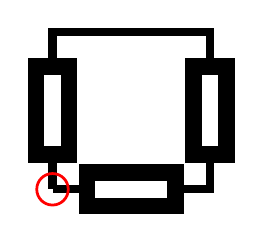
\begin{tikzpicture}[line width=3pt,european]
	\draw (0,0) to[R]++(2,0)to[R]++(0,2)
		--++(-2,0)to[R]++(0,-2);
	\draw[red,line width=1pt] circle(2mm);
	\end{tikzpicture}
\end{LTXexample}
To correct the line ending, there are support shapes to fill the missing rectangle. They can be used like the support shapes (*,o,d) using a dot (.) on one or both ends of a component (have a look at the last resistor in this example:
\begin{LTXexample}[varwidth=true]
	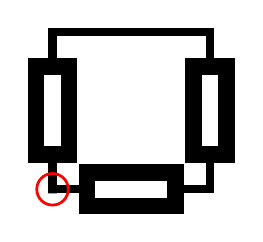
\begin{tikzpicture}[line width=3pt,european]
	\draw (0,0) to[R]++(2,0)to[R]++(0,2)
		--++(-2,0)to[R,-.]++(0,-2);
	\draw[red,line width=1pt] circle(2mm);
	\end{tikzpicture}
\end{LTXexample}


\section{Colors}

\subsection{Shape colors}

The color of the components is stored in the key \verb!\circuitikzbasekey/color!. Circui\TikZ\ tries to follow the color set in \TikZ, although sometimes it fails. If you change color in the picture, please do not use just the color name as a style, like \verb![red]!, but rather assign the style \verb![color=red]!.

Compare for instance
\begin{LTXexample}[varwidth=true]
\begin{circuitikz} \draw[red]
  (0,2) node[and port] (myand1)  {}
  (0,0) node[and port] (myand2)  {}
  (2,1) node[xnor port] (myxnor)  {}
  (myand1.out) -| (myxnor.in 1)
  (myand2.out) -| (myxnor.in 2)
;\end{circuitikz}
\end{LTXexample}

and

\begin{LTXexample}[varwidth=true]
\begin{circuitikz} \draw[color=red]
  (0,2) node[and port] (myand1)  {}
  (0,0) node[and port] (myand2)  {}
  (2,1) node[xnor port] (myxnor)  {}
  (myand1.out) -| (myxnor.in 1)
  (myand2.out) -| (myxnor.in 2)
;\end{circuitikz}
\end{LTXexample}

One can of course change the color \emph{in medias res}:
\begin{LTXexample}[pos=t, varwidth=true]
\begin{circuitikz} \draw
  (0,0) node[pnp, color=blue] (pnp2) {}
  (pnp2.B) node[pnp, xscale=-1, anchor=B, color=brown] (pnp1) {}
  (pnp1.C) node[npn, anchor=C, color=green] (npn1) {}
  (pnp2.C) node[npn, xscale=-1, anchor=C, color=magenta] (npn2) {}
  (pnp1.E) -- (pnp2.E)  (npn1.E) -- (npn2.E)
  (pnp1.B) node[circ] {} |- (pnp2.C) node[circ] {}
;\end{circuitikz}
\end{LTXexample}

The all-in-one stream of bipoles poses some challanges, as only the actual body of the bipole, and not the connecting lines, will be rendered in the specified color. Also, please notice the curly braces around the \texttt{to}:
\begin{LTXexample}[varwidth=true]
\begin{circuitikz} \draw
  (0,0) to[V=1<\volt>] (0,2)
      { to[R=1<\ohm>, color=red] (2,2) }
        to[C=1<\farad>] (2,0) -- (0,0)
;\end{circuitikz}
\end{LTXexample}

Which, for some bipoles, can be frustrating:
\begin{LTXexample}[varwidth=true]
\begin{circuitikz} \draw
  (0,0){to[V=1<\volt>, color=red] (0,2) }
        to[R=1<\ohm>] (2,2)
        to[C=1<\farad>] (2,0) -- (0,0)
;\end{circuitikz}
\end{LTXexample}

The only way out is to specify different paths:
\begin{LTXexample}[varwidth=true]
\begin{circuitikz} \draw[color=red]
  (0,0) to[V=1<\volt>, color=red] (0,2);
  \draw (0,2) to[R=1<\ohm>] (2,2)
        to[C=1<\farad>] (2,0) -- (0,0)
;\end{circuitikz}
\end{LTXexample}

And yes: this is a bug and \emph{not} a feature\ldots

\subsection{Fill colors}

Since version 0.9.0, you can also fill most shapes with a color (the manual specifies which ones are fillable or not). The syntax is quite intuitive:

\begin{LTXexample}[varwidth=true]
\begin{circuitikz} \draw
    (0,2) node[and port, fill=yellow] (myand1)  {}
    (0,0) node[and port, fill=cyan] (myand2)  {}
    (2,1) node[xnor port,fill=red!30!white] (myxnor)  {}
  (myand1.out) -| (myxnor.in 1)
  (myand2.out) -| (myxnor.in 2)
;\end{circuitikz}
\end{LTXexample}

You can combine shape colors with fill colors, too, but you should use the \texttt{draw} color option style for this:

\begin{LTXexample}[varwidth=true]
\begin{circuitikz} \draw[color=red]
    (0,2) node[and port, fill=yellow] (myand1)  {1}
    (0,0) node[and port, fill=cyan] (myand2)  {2}
    (2,1) node[xnor port,fill=red!30!white] (myxnor)  {3}
  (myand1.out) -| (myxnor.in 1)
  (myand2.out) -| (myxnor.in 2)
;\end{circuitikz}
\end{LTXexample}

This is because, as you can see from the following example in port \texttt{2}, you can't specify both a fill and a color in the node (yes, it's a bug too, but it's quite complex to solve given the current circuit\TikZ{} architecture).  a workaround is shown in port \texttt{3}:


\begin{LTXexample}[varwidth=true]
\begin{circuitikz} \draw
  (0,2) node[and port, color=black] (myand1)  {1}
  (0,0) node[and port, color=blue, fill=cyan] (myand2)  {2}
  (2,1) {[color=blue] node[xnor port, fill=cyan] (myxnor)  {3}}
  (myand1.out) -| (myxnor.in 1)
  (myand2.out) -| (myxnor.in 2)
;\end{circuitikz}
\end{LTXexample}

Notice also that the connection point are always filled, although the color \emph{tries} to follow the color of the filling of the component:

\begin{LTXexample}[varwidth=true, pos=t]
\begin{circuitikz}
    \fill[cyan] (0,3.0) rectangle (7,7);
    \draw [fill=yellow, ] (4,4) to [D,o-o] ++(0,2) to[D*, fill=yellow] ++(2,0)
    to[D*] ++(0,-2)  to[D, fill=red, o-o] ++(-2,0);
    \draw (1,4) node[ocirc]{} -- ++(1,0) node[ocirc]{};
    \draw (1,4.5) to[short, o-o] ++(1,0) to[short, -o] ++(1,0);
    \draw[fill=yellow] (1,5) to[short, o-o] ++(1,0) to[short, -o] ++(1,0);
    \draw (1,5.5) to[short, fill=red, o-o] ++(1,0) to[short, -o] ++(1,0);
\end{circuitikz}
\end{LTXexample}

\section{FAQ}

\noindent Q: When using \verb!\tikzexternalize! I get the following error:
\begin{verbatim}
 ! Emergency stop.
\end{verbatim}

\noindent A: The \TikZ\ manual states:
\begin{quotation}
Furthermore, the library assumes that all \LaTeX\ pictures are ended
    with \\\verb!\end{tikzpicture}!.
\end{quotation}

Just substitute every occurrence of the environment \verb!circuitikz! with \verb!tikzpicture!. They are actually pretty much the same.

\bigskip

\noindent Q: How do I draw the voltage between two nodes?

\noindent A: Between any two nodes there is an open circuit!
\begin{LTXexample}[varwidth=true]
\begin{circuitikz} \draw
  node[ocirc] (A) at (0,0) {}
  node[ocirc] (B) at (2,1) {}
  (A) to[open, v=$v$] (B)
;\end{circuitikz}
\end{LTXexample}

\bigskip

\noindent Q: I cannot write \verb!to[R = $R_1=12V$]! nor \verb!to[ospst = open, 3s]!: I get errors.

\noindent A: It is a limitation of the parser.

Use \verb|\def{\eq}{=}|  \verb!to[R = $R_1\eq 12V$]! and  \verb!to[ospst = open{,} 3s]! instead; see caveat in section~\ref{sec:labels-and-annotations}.

\bigskip

\noindent Q: I tried to change the direction of the $y$ axis with \texttt{yscale=-1}, but the circuit is completely messed up.

\noindent A: Yes, it's a known bug (or misfeature, or limitation). See section~\ref{sec:bugs}. Don't do that.


\bigskip

\noindent Q: I tried to put a diode in a \texttt{pic}, but it's coming out badly rotated.

\noindent A: Yes, it's a known bug (or misfeature, or limitation). See section~\ref{sec:bugs}. \Circuitikz{} is not compatible with \texttt{pic}s at this point.

\section{Defining new components}

\begin{quote}
    Per me si va ne la città dolente,\\
    per me si va ne l'etterno dolore,\\
    per me si va tra la perduta gente.\\
    \dots\\
    Lasciate ogne speranza, voi ch'intrate.%
    \footnote{\url{https://classicsincontext.wordpress.com/2010/02/28/canto-iii-per-me-si-va-ne-la-citta-dolente/}}
\end{quote}


\textbf{Big fat warning}: this material is reserved to \TeX-hackers; do not delve into this if you have no familiarity with (at least) a bit of core \TeX{} programming and to the basic \TikZ{} layer. You have been warned.


\subsection{Suggested setup}

The suggested way to start working on a new component is to use the utilities of the \Circuitikz{} manual for checking and testing your device. Basically, find (or download) the source code of the last version of \Circuitikz{} and find the file \texttt{ctikzmanutils.sty}; copy it in your directory and prepare a file like this:

\begin{lstlisting}
\documentclass[a4paper, titlepage]{article}
\usepackage{a4wide}	%smaller borders
\usepackage[utf8]{inputenc}
\usepackage[T1]{fontenc}
\parindent=0pt
\parskip=4pt plus 6pt minus 2pt
\usepackage[siunitx, RPvoltages]{circuitikz}
\usepackage{ctikzmanutils}
\makeatletter
%%  Test things here
% defines

% components

% paths
\makeatother

\begin{document}

\circuitdescbip*{damper}{Mechanical damping}{}(left/135/0.2, right/45/0.2, center/-90/0.3)

\geolrcoord{dampershape, fill=yellow}

\begin{LTXexample}[varwidth]
\begin{circuitikz}
    \draw (0,0) to[R] ++(2,0)
    to[damper] ++(2,0);
\end{circuitikz}
\end{LTXexample}
\end{document}
\end{lstlisting}

This will compile to something like this (in this case, we are using a couple of existing components to check everything is ok):

\circuitdescbip*{damper}{Mechanical damping}{}(left/135/0.2, right/45/0.2, center/-90/0.3)

\geolrcoord{dampershape, fill=yellow}

\begin{LTXexample}[varwidth]
\begin{circuitikz}
    \draw (0,0) to[R] ++(2,0)
    to[damper] ++(2,0);
\end{circuitikz}
\end{LTXexample}

The command \verb|circuitdescbip*| is used to show the component description (you can check the definition and the usage looking at \texttt{ctikzmanutils.sty} file, and the \verb|\geolrcoord| is used to show the main anchors (geographical plus \texttt{left} and \texttt{right}) of the component.

From now on, you can add the new commands for the component between the \verb|\makeatletter| and \verb|\makeatother| commands and, modifying the example, check the results.

\subsection{Path-style component}

Let's define for example a path style component, like the one suggested by the user \texttt{@alex} on \href{https://tex.stackexchange.com/questions/484268/combined-spring-damper-in-circuitikz}{tex.stackexchange.com}. The component will be a mix of the \texttt{damper} and the \texttt{spring} components already present.

The first step is to check if we can use the definition already existing for similar elements (for coherence of size) or if we need to define new ones; for this you have to check the file \texttt{pgfcirc.defines.tex}: we find

\begin{lstlisting}
    \ctikzset{bipoles/spring/height/.initial=.5}
    \ctikzset{bipoles/spring/width/.initial=.5}
    \ctikzset{bipoles/damper/height/.initial=.35}
    \ctikzset{bipoles/damper/length/.initial=.3}
    \ctikzset{bipoles/damper/width/.initial=.4}
\end{lstlisting}

We will use them; at this stage you can decide to add other parameters if you need them. (Notice, however, than although flexibility is good, these parameters should be described in the manual, otherwise they're as good as a fixed number in the code).


To define the new component we will look into \texttt{pgfcircbipoles.tex} and we will copy, for example, the definition of the damper into our code, just changing the name:

\begin{lstlisting}
%% mechanical resistor - damper
\pgfcircdeclarebipole
{}                                   % extra anchors
{\ctikzvalof{bipoles/damper/height}} % depth (under the path line)
{viscoe}                             % name
{\ctikzvalof{bipoles/damper/height}} % height (above the path line)
{\ctikzvalof{bipoles/damper/width}}  % width
{ % draw the bipole
    \pgfpathrectanglecorners{\pgfpoint{\ctikzvalof{bipoles/damper/length}\pgf@circ@res@right}{\pgf@circ@res@down}}{\pgfpoint{\pgf@circ@res@right}{\pgf@circ@res@up}}
    \pgf@circ@maybefill

    % line into the damper
    \pgfpathmoveto{\pgfpoint{\pgf@circ@res@left}{\pgf@circ@res@zero}}
    \pgfpathlineto{\pgfpoint{\ctikzvalof{bipoles/damper/length}\pgf@circ@res@right}
        {\pgf@circ@res@zero}}
    \pgfusepath{stroke}

    % damper box
    \pgfsetlinewidth{\pgfkeysvalueof{/tikz/circuitikz/bipoles/thickness}\pgfstartlinewidth}
    \pgfpathmoveto{\pgfpoint{\pgf@circ@res@left}{\pgf@circ@res@down}}
    \pgfpathlineto{\pgfpoint{\pgf@circ@res@right}{\pgf@circ@res@down}}
    \pgfpathlineto{\pgfpoint{\pgf@circ@res@right}{\pgf@circ@res@up}}
    \pgfpathlineto{\pgfpoint{\pgf@circ@res@left}{\pgf@circ@res@up}}

    \pgfsetrectcap
    \pgfsetmiterjoin
    \pgfusepath{stroke}

    % damper vertical element
    \pgfpathmoveto{\pgfpoint{\ctikzvalof{bipoles/damper/length}\pgf@circ@res@right}
        {.8\pgf@circ@res@down}}
    \pgfpathlineto{\pgfpoint{\ctikzvalof{bipoles/damper/length}\pgf@circ@res@right}
        {.8\pgf@circ@res@up}}
    \pgfsetbuttcap
    \pgfusepath{stroke}
}
\end{lstlisting}

This command will define a shape that is named \texttt{viscoeshape}, with all the correct geographical anchors based on the depth, height and width defined in the parameters of \verb|\pgfcircdeclarebipole|. This is not sufficient for using the element in a \texttt{to[]} path command; you need to ``activate'' it with (this commands are normally in \texttt{pgfcircpath.tex}):

\begin{lstlisting}
\def\pgf@circ@viscoe@path#1{\pgf@circ@bipole@path{viscoe}{#1}}
\compattikzset{viscoe/.style = {\circuitikzbasekey,
        /tikz/to path=\pgf@circ@dviscoe@path, l=#1}}
\end{lstlisting}

And now you can show it with:

\begin{lstlisting}
\circuitdescbip*{viscoe}{Mechanical viscoelastic element\footnotemark}{}(left/135/0.2, right/45/0.2, center/-90/0.3)

\geolrcoord{viscoeshape, fill=yellow}

\begin{LTXexample}[varwidth]
\begin{circuitikz}
    \draw (0,0) to[spring] ++(2,0)
    to[viscoe] ++(2,0);
\end{circuitikz}
\end{LTXexample}
\end{lstlisting}

Obviously, at first you you just have a component that is the same as the one you copied with another name. It is now just a matter of modifying it so that it has the desired shape; in the example above you can already see the new symbol after the changes.

When doing the drawing, the \verb|\pgfcircdeclarebipole| will setup the lengths \verb|\pgf@circ@res@right|
and \verb|\pgf@circ@res@up| as the $x$-$y$ coordinates of the upper right corner, and
\verb|\pgf@circ@res@left|  and \verb|\pgf@circ@res@down| as the $x$-$y$ coordinates of the lower left corner of your shape. The \texttt{center} coordinate is usually at $(0pt, 0pt)$.

Looking at the implementation of the \texttt{spring} element, a possible implementation is changing the lines between  lines~12 and~16 with:

\begin{lstlisting}
    % spring into the damper
    \pgfscope
        \pgfpathmoveto{\pgfpoint{\pgf@circ@res@left}{\pgf@circ@res@zero}}
        \pgfsetlinewidth{\pgfkeysvalueof{/tikz/circuitikz/bipoles/thickness}\pgfstartlinewidth}
        \pgfsetcornersarced{\pgfpoint{.25\pgf@circ@res@up}{.25\pgf@circ@res@up}}
        \pgfpathlineto{\pgfpoint{.75\pgf@circ@res@left}{.75\pgf@circ@res@up}}
        \pgfpathlineto{\pgfpoint{.5\pgf@circ@res@left}{-.75\pgf@circ@res@up}}
        \pgfpathlineto{\pgfpoint{.25\pgf@circ@res@left}{.75\pgf@circ@res@up}}
        \pgfpathlineto{\pgfpoint{0pt}{-.75\pgf@circ@res@up}}
        \pgfpathlineto{\pgfpoint{\ctikzvalof{bipoles/damper/length}\pgf@circ@res@right}{.75\pgf@circ@res@up}}
        \pgfusepath{stroke}
    \endpgfscope
\end{lstlisting}

which leads to:

\circuitdescbip*{viscoe}{Mechanical viscoelastic element}{}(left/135/0.2, right/45/0.2, center/-90/0.3)

\geolrcoord{viscoeshape, fill=yellow}

\begin{LTXexample}[varwidth]
\begin{circuitikz}
    \draw (0,0) to[spring] ++(2,0)
    to[viscoe] ++(2,0);
\end{circuitikz}
\end{LTXexample}


As a final note, notice that the \texttt{viscoe} element is already added to the standard package.

\subsection{Node-style component}

Adding a node-style component is much more straightforward. Just define it by following examples in, for example, \texttt{pgfcirctripoles.tex} or the other files; be careful that you should define all the geographical anchors of the shape if you want that the \TikZ{} positioning options (like \texttt{left}, \texttt{above}, etc.) behave correctly with your component.

\subsubsection{Finishing your work}

Once you have a satisfactory element, you should
\begin{itemize}
    \item Clean up your code;
    \item write a piece of documentation explaining its use, with an example;
    \item Propose the element for inclusion in the GitHub page of the project (you will have to license this as explained in that page, of course).
\end{itemize}

The best way of contributing is forking the project, adding your component in the correct files, modifying the manual and creating a pull request for the developers to merge.  Anyway, if this is a problem, just open an issue and someone (when they have time\dots) will answer.



\section{Examples}

\begin{LTXexample}[pos=t,varwidth=true]
\begin{circuitikz}[scale=1.4]\draw
  (0,0) to[C, l=10<\micro\farad>] (0,2) -- (0,3)
        to[R, l=2.2<\kilo\ohm>] (4,3) -- (4,2)
        to[L, l=12<\milli\henry>, i=$i_1$,v=b] (4,0) -- (0,0)
  (4,2) { to[D*, *-*, color=red] (2,0) }
  (0,2) to[R, l=1<\kilo\ohm>, *-] (2,2)
        to[cV, i=1,v=$\SI{.3}{\kilo\ohm} i_1$] (4,2)
  (2,0) to[I, i=1<\milli\ampere>, -*] (2,2)
;\end{circuitikz}
\end{LTXexample}

\begin{LTXexample}[pos=t,varwidth=true]
\begin{circuitikz}[scale=1.2]\draw
  (0,0) node[ground] {}
        to[V=$e(t)$, *-*] (0,2) to[C=4<\nano\farad>] (2,2)
        to[R, l_=.25<\kilo\ohm>, *-*] (2,0)
  (2,2) to[R=1<\kilo\ohm>] (4,2)
        to[C, l_=2<\nano\farad>, *-*] (4,0)
  (5,0) to[I, i_=$a(t)$, -*] (5,2) -- (4,2)
  (0,0) -- (5,0)
  (0,2) -- (0,3) to[L, l=2<\milli\henry>] (5,3) -- (5,2)

 {[anchor=south east] (0,2) node {1} (2,2) node {2} (4,2) node {3}}
;\end{circuitikz}
\end{LTXexample}

\begin{LTXexample}[pos=t,varwidth=true]
\begin{circuitikz}[scale=1.2]\draw
  (0,0) node[anchor=east] {B}
        to[short, o-*] (1,0)
        to[R=20<\ohm>, *-*] (1,2)
        to[R=10<\ohm>, v=$v_x$] (3,2) -- (4,2)
        to[cI=$\frac{\siemens}{5} v_x$, *-*] (4,0) -- (3,0)
        to[R=5<\ohm>, *-*] (3,2)
  (3,0) -- (1,0)
  (1,2) to[short, -o] (0,2) node[anchor=east]{A}
;\end{circuitikz}
\end{LTXexample}

\begin{LTXexample}[pos=t,varwidth=true]
\begin{circuitikz}[scale=1]\draw
	(0,0) node[transformer] (T) {}
	(T.B2) to[pD] ($(T.B2)+(2,0)$) -| (3.5, -1)
	(T.B1) to[pD] ($(T.B1)+(2,0)$)  -| (3.5, -1)
;\end{circuitikz}
\end{LTXexample}


\begin{LTXexample}[pos=t,varwidth=true]
\begin{circuitikz}[scale=1]\draw
    (5,.5) node [op amp] (opamp) {}
    (0,0) node [left] {$U_{we}$} to [R, l=$R_d$, o-*] (2,0)
    to [R, l=$R_d$, *-*] (opamp.+)
    to [C, l_=$C_{d2}$, *-] ($(opamp.+)+(0,-2)$) node [ground] {}
    (opamp.out) |- (3.5,2) to [C, l_=$C_{d1}$, *-] (2,2) to [short] (2,0)
    (opamp.-) -| (3.5,2)
    (opamp.out) to [short, *-o] (7,.5) node [right] {$U_{wy}$}
;\end{circuitikz}
\end{LTXexample}

\begin{LTXexample}[pos=t,varwidth=true]
\begin{circuitikz}[scale=1.2, american]\draw
  (0,2) to[I=1<\milli\ampere>] (2,2)
        to[R, l_=2<\kilo\ohm>, *-*] (0,0)
        to[R, l_=2<\kilo\ohm>] (2,0)
        to[V, v_=2<\volt>] (2,2)
        to[cspst, l=$t_0$] (4,2) -- (4,1.5)
        to [generic, i=$i_1$, v=$v_1$] (4,-.5) -- (4,-1.5)
  (0,2) -- (0,-1.5) to[V, v_=4<\volt>] (2,-1.5)
        to [R, l=1<\kilo\ohm>] (4,-1.5);

   \begin{scope}[xshift=6.5cm, yshift=.5cm]
    \draw [->] (-2,0) -- (2.5,0) node[anchor=west] {$v_1/\volt$};
    \draw [->] (0,-2) -- (0,2) node[anchor=west] {$i_1/\SI{}{\milli\ampere}$} ;
    \draw (-1,0) node[anchor=north] {-2} (1,0) node[anchor=south] {2}
          (0,1) node[anchor=west] {4} (0,-1) node[anchor=east] {-4}
          (2,0) node[anchor=north west] {4}
          (-1.5,0) node[anchor=south east] {-3};
    \draw [thick] (-2,-1) -- (-1,1) -- (1,-1) -- (2,0) -- (2.5,.5);
    \draw [dotted] (-1,1) -- (-1,0) (1,-1) -- (1,0)
          (-1,1) -- (0,1) (1,-1) -- (0,-1);
   \end{scope}
\end{circuitikz}
\end{LTXexample}

\begin{LTXexample}[pos=t,varwidth=true]
    \begin{circuitikz}[scale=1]
        \ctikzset{bipoles/detector/width=.35}
        \ctikzset{quadpoles/coupler/width=1}
        \ctikzset{quadpoles/coupler/height=1}
        \ctikzset{tripoles/wilkinson/width=1}
        \ctikzset{tripoles/wilkinson/height=1}
        %\draw[help lines,red,thin,dotted] (0,-5) grid (5,5);
        \draw
        (-2,0) node[wilkinson](w1){}
        (2,0) node[coupler] (c1) {}
        (0,2) node[coupler,rotate=90] (c2) {}
        (0,-2) node[coupler,rotate=90] (c3) {}
        (w1.out1) .. controls ++(0.8,0) and ++(0,0.8) .. (c3.3)
        (w1.out2) .. controls ++(0.8,0) and ++(0,-0.8) .. (c2.4)
        (c1.1) .. controls ++(-0.8,0) and ++(0,0.8) .. (c3.2)
        (c1.4) .. controls ++(-0.8,0) and ++(0,-0.8) .. (c2.1)
        (w1.in) to[short,-o] ++(-1,0)
        (w1.in) node[left=30] {LO}
        (c1.2) node[match,yscale=1] {}
        (c1.3) to[short,-o] ++(1,0)
        (c1.3) node[right=30] {RF}
        (c2.3) to[detector,-o] ++(0,1.5)
        (c2.2) to[detector,-o] ++(0,1.5)
        (c3.1) to[detector,-o] ++(0,-1.5)
        (c3.4) to[detector,-o] ++(0,-1.5)
        ;
    \end{circuitikz}
\end{LTXexample}


\begin{tabular}{l}\label{ex:compatibility}
\IfFileExists{compatibility.pdf}
{\fbox{\includegraphics{compatibility.pdf}}}
\\
\begin{lstlisting}
\documentclass{standalone}

\usepackage{tikz}
\usetikzlibrary{circuits.ee.IEC}
\usetikzlibrary{positioning}

\usepackage[compatibility]{circuitikzgit}
\ctikzset{bipoles/length=.9cm}

\begin{document}
 \begin{tikzpicture}[circuit ee IEC]
  \draw (0,0) to [resistor={name=R}] (0,2)
	to[diode={name=D}] (3,2);
  \draw (0,0) to[*R=$R_1$] (1.5,0) to[*Tnpn] (3,0)
    to[*D](3,2);
 \end{tikzpicture}
\end{document}
	\end{lstlisting}
\end{tabular}

% % changelog.tex will be updated by makefile from CHANGELOG.md
\section{Changelog}
\IfFileExists{changelog.tex}
{\sloppy\input{changelog.tex}}
{The file changelog.tex was not found, run 'make changelog' at toplevel to generate it with pandoc from CHANGELOG.md}

\printindex

\end{document}
